\chapter{More Exact Wavefunctions}

\section{Introduction}

In Chapter 2 we discussed approximate wavefunctions for H$^+_2$
$\chi_{\ell} \pm \chi_r$ and for H$_2$ $\chi_{\ell} \chi_r \pm \chi_r
\chi_{\ell}$.  In this chapter we will consider some aspects of more
exact wavefunctions of these molecules and for the two-electron atom,
He. Our emphasis here will be on qualitative ideas.

We first examine the variational principle and later we use this principle to
examine some of the useful methods for calculating wavefunctions such as 
HF, GVB, and CI.

Accurate wavefunctions for H$^+_2$, He, and H$_2$ are discussed in Sections 
3.3, 3.7, and 3.8, respectively. In Section 3.4 we re-examine the nature of 
the bond in H$^+_2$ and in Section 3.8 we re-examine the bond in H$_2$

The energy $\epsilon_0$  of any approximate wavefunction $\varphi_0$ is an 
upper bound on the exact energy of the ground state $E_0$,
\begin{equation}
\epsilon_0 \geq E_0 ,
\end{equation}
leading to the variational condition. If an approximate wavefunction, and 
hence the energy, is a function of some parameter $\lambda$, then the optimum 
wavefunction satisfies the necessary condition
\begin{equation}
{\partial \epsilon \over \partial \lambda} = 0 .
\end{equation}
Expanding the unknown wavefunction $\varphi$ in terms of a basis
\begin{equation}
\varphi = \sum^{p}_{\mu = 1} C_{\mu} \chi_{\mu}
\end{equation}
and applying the variational condition, leads to a set of matrix equations,
\begin{equation}
{\bf H} {\bf C} = E {\bf S} {\bf C}
\end{equation}
for obtaining the optimum coefficients, i.e., wavefunction.

More exact wavefunctions of H$^+_2$ are also considered, but later we find 
that the description of bonding, in terms of exchange energies is retained. In 
Section 3.6 we present an overview of three useful methods for 
wavefunctions. They are, first, the \emph{Hartree-Fock} (HF) method, a
generalization of the MO wavefunction in which the 
wavefunction (ground state of a two- electron system) is taken as
\begin{equation}
\Phi^{HF} ( 1 , 2 ) = \varphi ( 1 ) \varphi ( 2 )
\end{equation}
and the orbitals $\varphi$ optimized by solving the differential equation
\begin{equation}
H^{HF} \varphi = \left( h + J_{\varphi} \right) \varphi = \epsilon
\varphi
\label{chap3-eqno1}
\end{equation}
or the matrix equation
\begin{equation}
\mathbf{H}^{HF} \mathbf{C} = \epsilon \mathbf{S} 
\mathbf{C}.
\label{chap3-eqno2}
\end{equation}
These equations are nonlinear and must be solved iteratively.

Secondly, the \emph{generalized valence bond} (GVB) method, a
generalization of the VB method with the wavefunction taken of the
form
\begin{equation}
\Phi^{GVB} (1 , 2) = \varphi_a (1) \varphi_b (2) + \varphi_b (1) \varphi_a (2)
\end{equation}
and the orbitals $\varphi_a$ and $\varphi_b$ optimized. This leads to two 
matrix equations
\begin{equation}
\mathbf{H}^a \mathbf{C}_a = \epsilon_a \mathbf{S} \mathbf{C}_a
\end{equation}
\begin{equation}
\mathbf{H}^b \mathbf{C}_b = \epsilon_b \mathbf{S} \mathbf{C}_b
\end{equation}
analogous to the HF equations (\ref{chap3-eqno2}) and to two
differential equations analogous to (\ref{chap3-eqno1}).

Third, the \emph{configuration interaction} (CI) method with the
wavefunction taken of the form
\begin{equation}
\Phi^{CI} (1, 2) = \sum_{\mu , \nu} C_{\mu \nu} \chi_{\mu} ( 1 ) 
\chi_{\nu} ( 2 )
\end{equation}
For the ground state this wavefunction can always be written in terms of
natural orbitals $\{ {\bar{\chi}}_{\mu} \}$ as
\begin{equation}
\Phi^{CI} (1, 2) = \sum_{\mu} {\bar{C}}_{\mu \nu} {\bar{\chi}}_{\mu} ( 1 ) 
{\bar{\chi}}_{\nu} ( 2 ) .
\end{equation}

Later in Section 3.6 we find that the ground state of any two electron 
systems is nodeless and symmetric
\begin{equation}
\Phi (1 , 2) = \Phi (2 , 1).
\end{equation}

In Sections 3.7 and 3.8 we find that the HF wavefunction accounts for
all but about 1.1 eV of the energy for He and H$_2$, and that a CI
wavefunction with five natural orbitals accounts for all but about
0.15 eV. The four correlating natural orbitals for this wavefunction
all involve one nodal plane.

All of these methods involve expansions in terms of basis sets. For He
it is possible to obtain highly accurate HF and GVB wavefunctions with
only two, $s$-like, basis functions. The \emph{double valence} (DV)
basis and for H$_2$ similar quality wavefunctions can be obtained with
six basis functions, two $s$ and one $p$ on each center, the
\emph{double valence plus polarization}(DVP) basis.

\section{The Variational Principle}

The wavefunction for the ground state of the hydrogen atom has the
form $e^{-r}$, and the wavefunction for the ground state of the
harmonic oscillator is $e^{- \alpha r^2}$.  However, there are very
few interesting systems for which the Schr\"odinger equation can be
solved exactly. Even so, there are general procedures allowing one to
obtain highly accurate, indeed arbitrarily accurate,
wavefunctions. The powerful tool needed is the \emph{variational
principle}. Here, we will outline some of the key results of this
principle.

\subsection{Upper Bound Theorem}

If $\psi_0$ and $E_0$ are the exact ground state wavefunction, and energy 
of a system
\begin{equation}
H \psi_0 = E_0 \psi_0
\end{equation}
and if $\varphi_0$ is an approximate wavefunction with energy
\begin{equation}
\epsilon_0 = {\langle \varphi_0 \vert H \vert \varphi_0 \rangle 
\over \langle \varphi_0 \vert \varphi_0 \rangle} ,
\end{equation}
then
\begin{equation}
\epsilon_0 \geq E_0 .
\label{chap3-eqno3}
\end{equation}
That is, the energy evaluated using any approximate wavefunction is an 
upper bound in the exact energy of the ground state.

\subsection{Variational Condition}

Given an approximate wavefunction $\varphi_{\lambda}(r)$  depending upon 
some parameter $\lambda$, e.g.,
\begin{equation}
\varphi_{\lambda} = e^{- \lambda r} ,
\end{equation}
then the optimum value of $\lambda$, for describing the system, must satisfy 
the necessary condition
\begin{equation}
{\partial \epsilon ( \lambda ) \over \partial \lambda} = 0 ,
\label{chap3-eqno4}
\end{equation}
where
\begin{equation}
\epsilon ( \lambda ) = {\langle \varphi_{\lambda} \vert H \vert 
\varphi_{\lambda} \rangle \over \langle \varphi_{\lambda} \vert 
\varphi_{\lambda} \rangle} .
\end{equation}
Equation (\ref{chap3-eqno4}) is referred to as the \emph{variational
condition}.

\subsection{Basis Set Expansions}

Given a set of functions
\begin{equation}
\left\{ \chi_{\mu} ( r ) , \mu = 1 , 2 , \cdot \cdot \cdot , P 
\right\} ,
\label{chap3-eqno5}
\end{equation}
the optimum wavefunction of the form
\begin{equation}
\varphi = \sum^{p}_{\mu = 1} C_{\mu} \chi_{\mu}
\label{chap3-eqno6}
\end{equation}
satisfies the condition
\begin{equation}
\sum_{\nu} H_{\mu \nu} C_{\nu} = E \sum_{\nu} S_{\mu \nu} C_{\nu},
\label{chap3-eqno7a}
\end{equation}
or in matrix notation
\begin{equation}
{\bf H} {\bf C} = E {\bf S} {\bf C},
\label{chap3-eqno7b}
\end{equation}
where
\begin{equation}
H_{\mu \nu} \equiv \langle \chi_{\mu} \vert H \vert \chi_{\nu} 
\rangle 
\label{chap3-eqno8a}
\end{equation}
and
\begin{equation}
S_{\mu \nu} \equiv \langle \chi_{\mu} \vert \chi_{\nu} \rangle 
.
\label{chap3-eqno8b}
\end{equation}
The set of functions (\ref{chap3-eqno5}) used for expansion of the
unknown function $\varphi$, is called a basis set. The unknowns are
the coefficients
\begin{equation}
\left\{ C_{\mu} ; \mu = 1 , \cdot \cdot \cdot , P \right\}
\end{equation}
which are obtained by solving the matrix equations
\ref{chap3-eqno7a}--\ref{chap3-eqno7b}. 

\subsection{Discussion of Upper Bound Theorem}

The upper bound theorem (\ref{chap3-eqno3}) is easy to
derive. Consider that the exact eigenstates $\{ \psi_i \}$ of the
Hamiltonian were known
\begin{equation}
H \psi_i = E_i \psi_i
\label{chap3-eqno9}
\end{equation}
with $i = 0$ as the ground state.

Since the set of functions $\{ \psi_i \}$ is complete, we can expand any 
approximate wavefunction $\varphi_0$ as
\begin{equation}
\varphi_0 = \sum_{i} C_i \psi_i .
\label{chap3-eqno10}
\end{equation}
Of course, in a real problem we will not know the functions $\{ \psi_i
\}$, and hence, we will not be able to calculate the $\{ C_i \}$.
However, the analysis in this section will serve to establish a
relation between the approximate and exact solutions. From equations
(\ref{chap3-eqno9}) and (\ref{chap3-eqno10})
\begin{equation}
H \varphi_0 = \sum_i C_i H \psi_i = \sum_i C_i E_i 
\psi_i
\end{equation}
and the energy of the approximate wavefunction $\psi_0$ is
\begin{equation}
\epsilon_0 \equiv \langle \varphi_0 \vert H \vert \varphi_0 
\rangle = \sum_i \sum_j C^*_j C_i E_i \langle \psi_j \vert \psi_i 
\rangle = \sum_i \vert C_i \vert^2 E_i .
\label{chap3-eqno11}
\end{equation}
Assuming $\varphi_0$ is normalized,
\begin{equation}
1 = \langle \varphi_0 \vert \varphi_0 \rangle = \sum_{ij} C^*_j C_i \langle 
\psi_j \vert \psi_i \rangle = \sum_i \vert C_i \vert^2 .
\label{chap3-eqno12}
\end{equation}
Using (\ref{chap3-eqno12}) in (\ref{chap3-eqno11}), we obtain
\begin{equation}
\epsilon_0 - E_0 = \sum_i \vert C_i \vert^2 \left( E_i - E_0 \right) 
.
\label{chap3-eqno13}
\end{equation}
Since $E_i \geq E_0$ and $\vert C_i \vert^2 \geq 0$, the right-hand side 
of (\ref{chap3-eqno13}) is necessarily positive, and hence
\begin{equation}
\epsilon_0 - E_0 \geq 0
\end{equation}
or
\begin{equation}
\epsilon_0 \geq E_0 .
\label{chap3-eqno14}
\end{equation}
That is, the energy calculated for any wavefunction is never lower than the
exact energy for the ground state wavefunction. Thus, we say that 
$\epsilon_0$ is an upper bound on $E_0$.

In deriving (\ref{chap3-eqno14}), we assumed that $\varphi_0$ could be
expanded in terms of the eigenfunctions of $H$. For
example, if the boundary conditions for the system described by
(\ref{chap3-eqno9}) were such that all wavefunctions are antisymmetric,
then we could not allow $\varphi_0$ to contain a symmetric part.

\subsection{Discussion of the Variational Principle}

Since any approximate wavefunction must yield an energy above the
energy of the exact, ground state, wavefunction, we have a useful
criterion for improving approximate wavefunctions. Namely, if you can
find some change in the wavefunction that leads to a lower energy,
then do it. Then reject any change that increase the energy.
Ultimately, if we consider all possible changes in the wavefunction,
this procedure must yield the exact wavefunction.  Normally we lose
patience before considering all changes in the wavefunction, and
instead we consider functions of certain restricted classes. Here our
basic criterion for approximating the wavefunction will be to select
the function of our specific restricted class leading to the lowest
energy. If $\lambda$ is some variable parameter for the restricted set
of functions being considered, then the optimum wavefunction must
satisfy
\begin{equation}
{\partial E \over \partial \lambda} = 0
\label{chap3-eqno15}
\end{equation}
since otherwise a lower energy could be obtained by changing $\lambda$ a 
bit, as illustrated in Figure \ref{fig3-01}.

\begin{figure}
\begin{center}
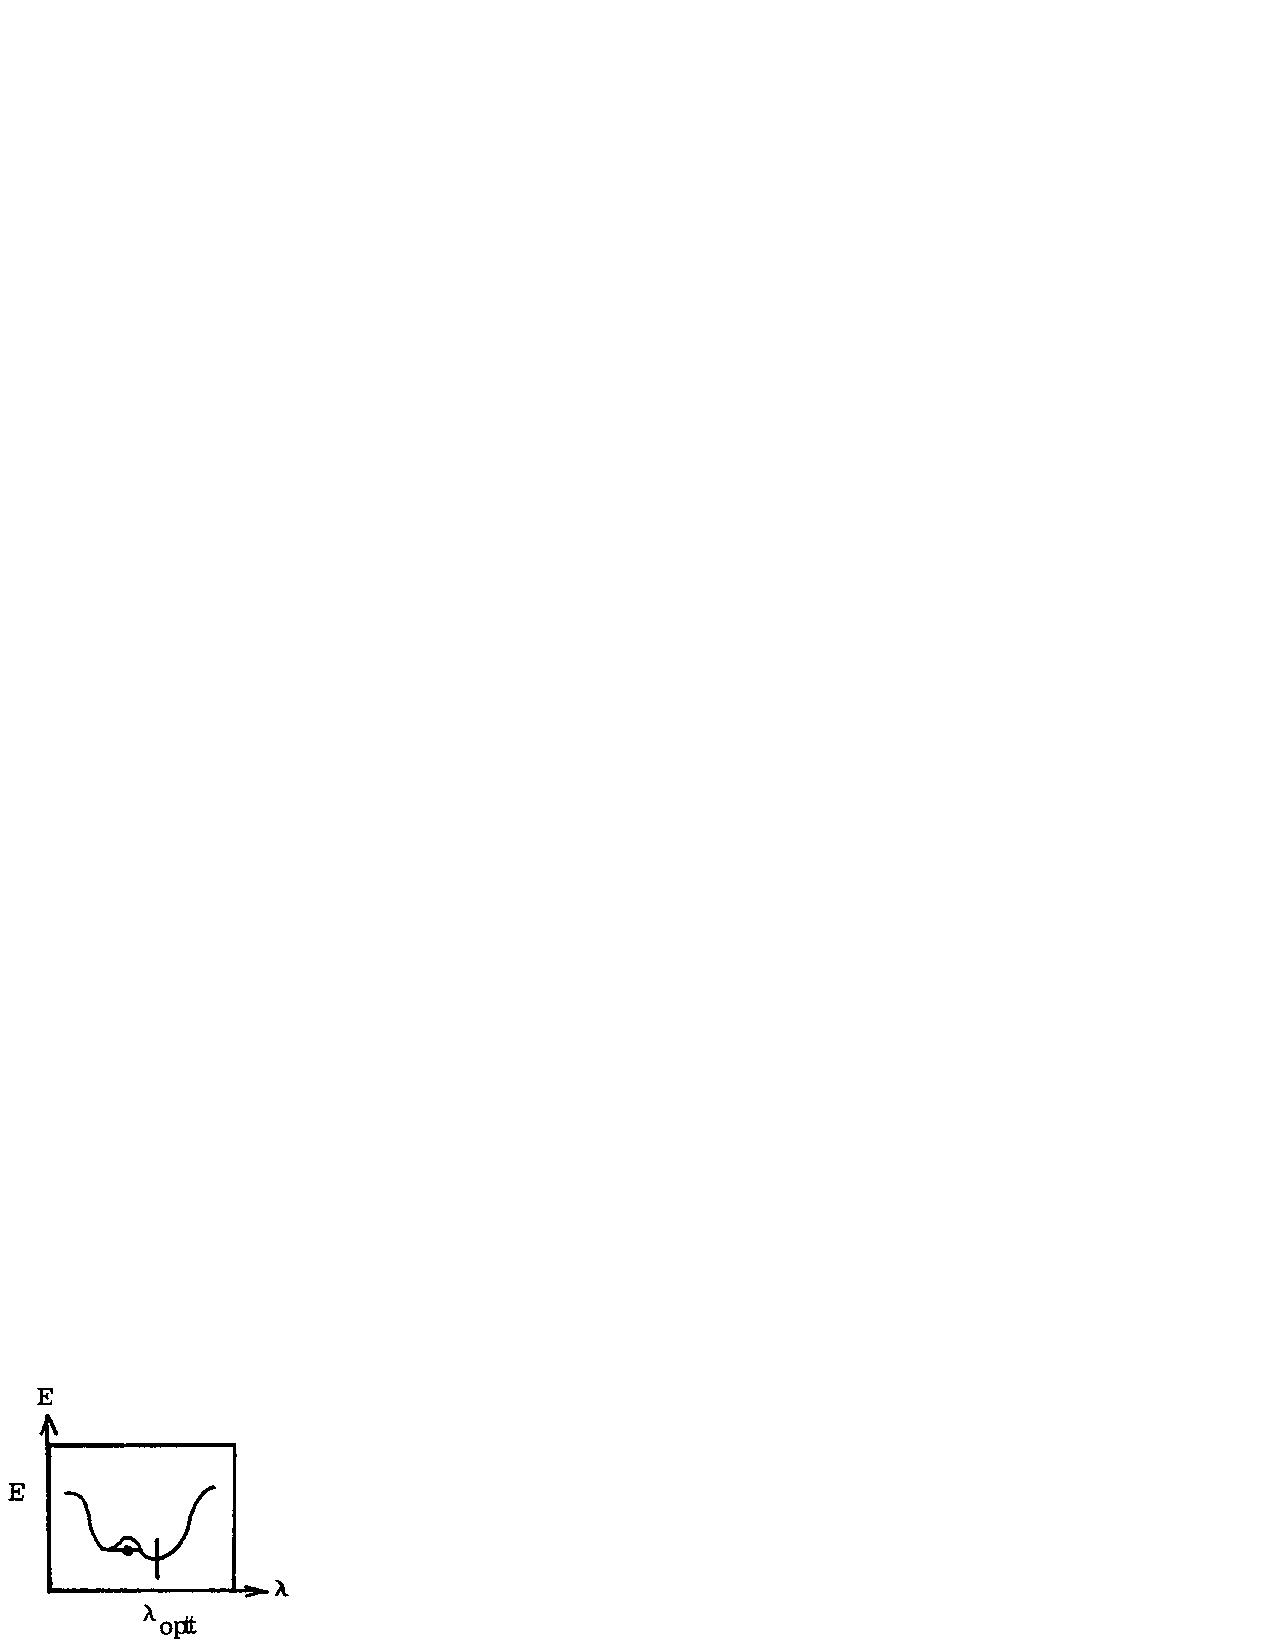
\includegraphics[scale=0.75]{fig3-01}
\end{center}
\caption{}
\label{fig3-01}
\end{figure}

\noindent
This criterion for optimizing a wavefunction is called the
\emph{variational principle} and forms the basis of all methods we
will consider for determining wavefunctions. It should be noted here
that (\ref{chap3-eqno15}) is not sufficient to guarantee a minimum, with
respect to variations in $\lambda$ (this requires 
${\partial^2 E \over \partial \lambda^2} > 0$)
and even if a minimum is found, it need not, in general, be the minimum 
leading to the lowest energy.  Fortunately, for the types of problems we 
deal with, these potential difficulties can usually be avoided.

\subsection{Parameter Optimization}

Consider, as an approximation to the ground state of the hydrogen atom, the
function
\begin{equation}
\varphi_0 ( \alpha ) = e^{- \alpha r^2}
\label{chap3-eqno16}
\end{equation}
where $\alpha$ is a parameter. To determine the value of $\alpha$
minimizing the energy, we first calculate the energy as a function of
$\alpha$,
\begin{equation}
E ( \alpha ) = {\langle \varphi_0 \vert - {1 \over 2} \nabla^2 - {1 
\over r} \vert \varphi_0 \rangle \over \langle \varphi_0 \vert \varphi_0 
\rangle} = {3 \over 2}\alpha - \left( {8 \over \pi \alpha} 
\right)^{{1 \over 2}}
\label{chap3-eqno17}
\end{equation}
The optimum value of $\alpha$ is given by
\begin{equation}
{dE ( \alpha ) \over d \alpha} = 0 = {3 \over 2} - {1 \over 2} \left( 
{8 \over \pi \alpha} \right)^{{1 \over 2}}
\end{equation}
or
\begin{equation}
\alpha_{opt} = {8 \over 9 \pi} = 0.283 ...
\end{equation}
Substituting this into (\ref{chap3-eqno17}), we obtain
\begin{equation}
E \left( \alpha_{opt} \right) = - {4 \over 3 \pi} = - 0.4244 ...
\end{equation}
recalling that the exact energy is $E = -0.5$. Thus, even though
(\ref{chap3-eqno16}) is considerably different from the exact
eigenfunction for the ground state of the hydrogen atom, by optimizing
$\alpha$ we are able to account for 84.9\% of the energy.

\subsection{Basis Set Expansions}

We will now use the variational principle to determine the best
representation of an approximate wavefunction as an expansion
(\ref{chap3-eqno6}), in terms of the functions of some finite basis
set (\ref{chap3-eqno5}). The energy is
\begin{equation}
E = {\langle \varphi \vert H \vert \varphi \rangle \over \langle 
\varphi \vert \psi \rangle} = {N \over D} ,
\label{chap3-eqno18}
\end{equation}
where
\begin{equation}
N = \sum_{\mu , \nu} C^*_{\mu} H_{\mu \nu} C_{\nu} ,
\end{equation}
\begin{equation}
D = \sum _{\mu , \nu} C^*_{\mu} S_{\mu \nu} C_{\nu},
\end{equation}
and, $H_{\mu \nu}$ and $S_{\mu \nu}$ are given in
(\ref{chap3-eqno8a})--(\ref{chap3-eqno8b}).  We do not assume here
that the basis functions are orthonormal; they must, of course, be
linearly independent.

The energy (\ref{chap3-eqno18}) depends on the $P$ parameters $\{
C_{\mu} \}$, and thus, from the variational principle we require that
\begin{equation}
{\partial E \over \partial C_{\mu}} = 0 ; \mu = 1 , 2 , \cdot \cdot 
\cdot , P.
\end{equation}
From (\ref{chap3-eqno18}), this leads to
\begin{equation}
{\partial E \over \partial C_{\mu}} = {1 \over D} {\partial N \over 
\partial C_{\mu}} - {N \over D^2} {\partial D \over \partial 
C_{\mu}} = {1 \over D} \left[ {\partial N \over \partial C_{\mu}} - 
E {\partial D \over \partial C_{\mu}} \right] = 0
\end{equation}
and hence,
\begin{equation}
{\partial N \over \partial C_{\mu}} - E {\partial D \over \partial 
C_{\mu}} = 0 .
\end{equation}
Assuming that the basis function $\{ \chi_{\mu} \}$ and coefficients 
$\{ C_{\mu} \}$ are all real, we obtain
\begin{equation}
2 \left[ \sum_{\nu} \left( H_{\mu \nu} - ES_{\mu \nu} \right) C_{\nu} 
\right] = 0
\end{equation}
and hence,
\begin{equation}
\sum_{\nu} H_{\mu \nu} C_{\nu}  E \sum_{\nu} S_{\mu \nu} C_{\nu} .
\label{chap3-eqno7-other}
\end{equation}
The more general case leads to the same equations.  Note that if the basis 
functions are real then $H_{\mu \nu} = H_{\nu \mu}$ and $S_{\mu \nu} = 
S_{\nu \mu}$.

In matrix notation, (\ref{chap3-eqno7-other}) becomes
\begin{equation}
{\bf H} {\bf C}  = E {\bf S} {\bf C}.
\label{chap3-eqno19}
\end{equation}

If the basis functions are orthonormal
\begin{equation}
S_{\mu \nu} = \delta_{\mu \nu} ,
\end{equation}
the variational condition (\ref{chap3-eqno19}) becomes
\begin{equation}
{\bf H} {\bf C} = E {\bf C}.
\label{chap3-eqno20}
\end{equation}
Thus, the variational principle leads to a finite matrix equation
directly analogous to the Schr\"odinger equation.  Indeed, if a
complete set of basis functions is used, the solution of
(\ref{chap3-eqno15}) or (\ref{chap3-eqno20}) is the exact solution of the
Schr\"odinger equation.  Although the wavefunction and basis functions
were written as one electron functions, this procedure applies
identically for many-electron wavefunctions.

\section{Accurate Wavefunctions for H$^+_2$}

The LCAO wavefunction of H$^+_2$ discussed in Chapter 2, is an
approximate wavefunction and does not provide a quantitatively
accurate description of H$^+_2$ near $R_e$.  In this section, we will
discuss more accurate wavefunctions of H$^+_2$. First we consider a
useful intermediate level description, the MBS wavefunction.


\subsection{Scaled LCAO Wavefunctions}

We will describe the wavefunction of H$^+_2$ in terms of linear combinations
of two orbitals, $\chi_\ell$ and $\chi_r$, centered on each proton, but rather 
than atomic orbitals, we will use scaled atomic-like orbitals
\begin{equation}
\chi_\ell = \sqrt{\left( {\zeta^3 \over \pi} \right)} e^{- \zeta 
r_a}
\label{chap3-eqno21a}
\end{equation}
and
\begin{equation}
\chi_r = \sqrt{\left( {\zeta^3 \over \pi} \right)} e^{- \zeta 
r_b}
\label{chap3-eqno21b}
\end{equation}
The scaling parameter $\zeta$ is referred to as an \emph{orbital
exponent}.  Use of $\zeta = 1$ leads to the LCAO description of
Chapter 2, $\zeta > 1$ leads to more contracted orbitals, while $\zeta
< 1$ leads to more diffuse orbitals.

Using the basis set (\ref{chap3-eqno21a})--(\ref{chap3-eqno21b}), the
wavefunctions of H$^+_2$ have the form
\begin{equation}
\varphi_g = {( \chi_\ell + \chi_r) \over \sqrt{2(1+S)}}
\end{equation}
\begin{equation}
\varphi_u = {( - \chi_\ell + \chi_r) \over \sqrt{2(1-S)}}
\end{equation}
just as in Chapter 2.  However, the energies of these wavefunctions
depend upon both $\zeta$ and $R$ (see Section \ref{appendix-a} in
Chapter 2 for the specific dependence of the integrals on $\zeta$).
At each $R$ we will use the $\zeta$ leading to the lowest energy.
Since the forms of $E_g$ and $E_u$ are different, the optimum $\zeta$
will be different for the $g$ and $u$ states, as shown in Figure
\ref{fig3-02}.

\begin{figure}
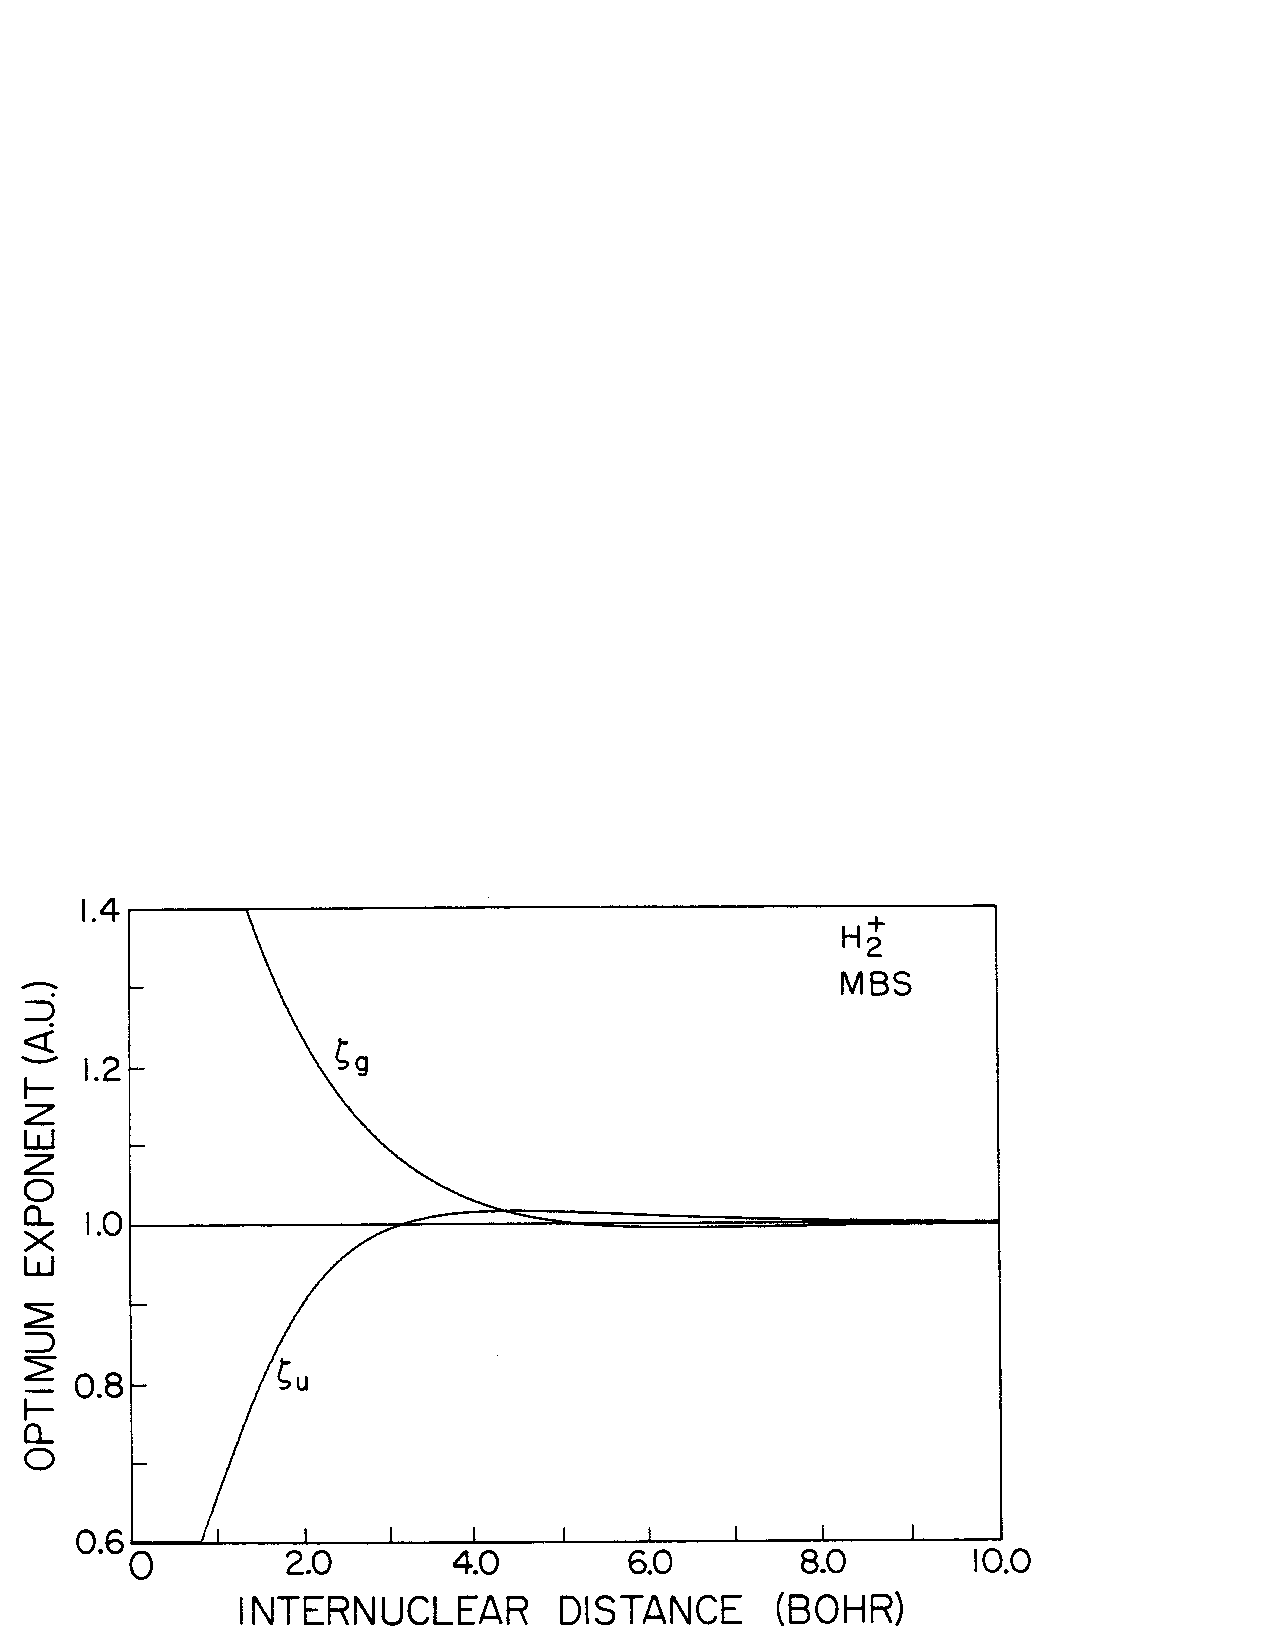
\includegraphics[scale=0.75]{fig3-01-1}
\caption{The optimal orbital exponents for the MBS descriptions of the
$g$ and $u$ states of H$_2^+$.}
\label{fig3-02}
\end{figure}

\begin{table}
\caption{Optimum bond length, $R_e$, and bond strength, 
$D_e$, for the $g$ state of H$^+_2$.  All quantities in atomic units.}
\label{table3-01}

\parindent=0.5truein

\begin{tabular}{cccccc}\\ \hline
&\multicolumn{3}{c}{Non-Relativistic} &
\multicolumn{2}{c}{Relativistic} \\

&\multicolumn{3}{c} {Neglect $T_{nuc}$} & Neglect $T_{nuc}$ &
Include $T_{nuc}$ \\

&LCAO$^a$ & MBS$^a$ & Exact$^b$ & Exact & Exact \\
$R_e$ & 2.493 & 2.00 & 2.00379$^c$ & 2.00376 $^c$ & 2.00562 $^c$ \\
$D_e$ & 0.065 & 0.08651 & 0.102635$^c$ & 0.10264$^c$ & 0.101785$^c$ \\
\hline  
\end{tabular}\\
$^a$See reference 1.  $^b$See reference 2. $^c$See reference 3. 
$^d$See reference 4.
\end{table}

As shown in Figure \ref{fig3-02} and seen in Table \ref{table3-01},
the improvement in the energy for the $g$ state is quite remarkable,
leading to energies close to the exact answer. For the $u$ state, both
the LCAO and the MBS
energies are quite close to the exact answer.


\begin{figure}
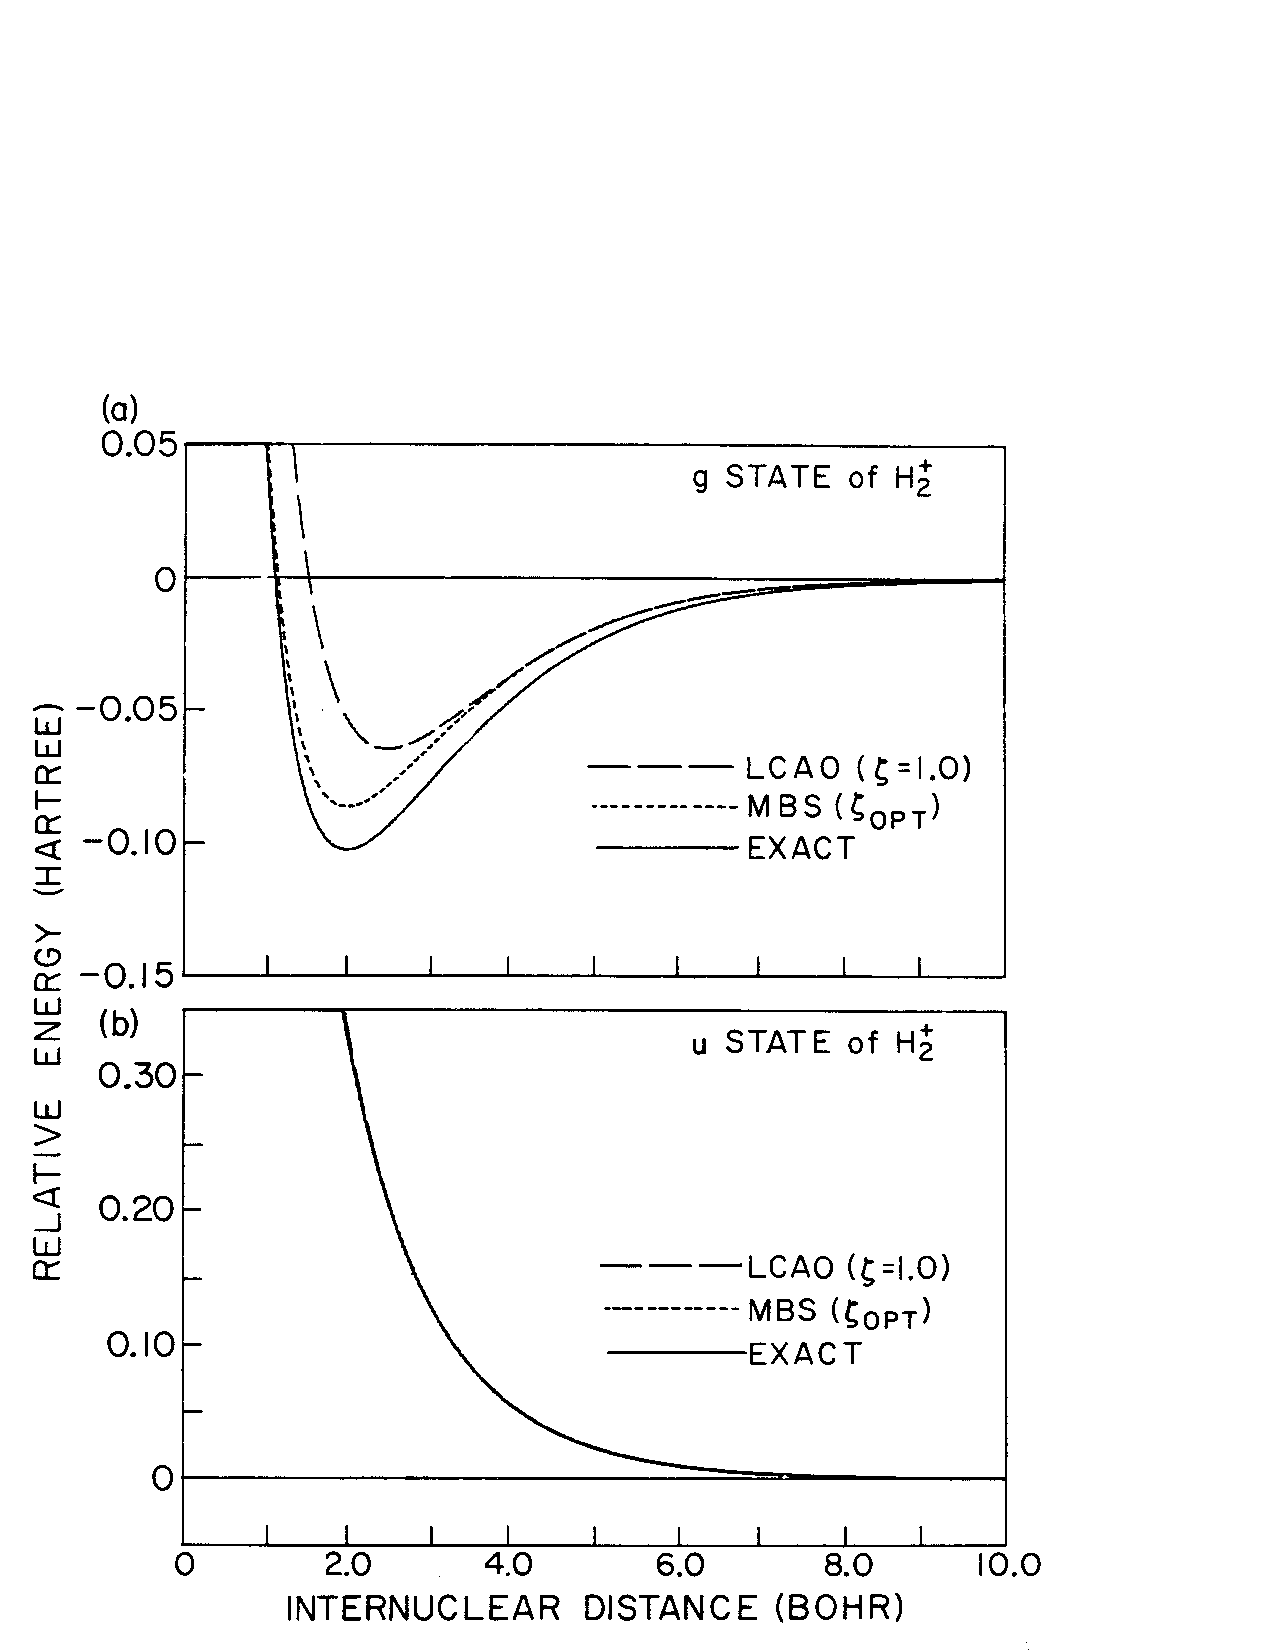
\includegraphics[scale=0.75]{fig3-02}
\caption{The LCAO ($\zeta=1.0$) MBS (optimum $\zeta$) and the exact
energies for the $g$ and $u$ states of H$^+_2$.  Note that (b)
does contain three different lines. The vertical scale of (b) is twice
that of (a).} 
\label{fig3-03}
\end{figure}

In discussing such wavefunctions, we will use the following terminology.
First, linear combination of atomic orbitals, LCAO, denotes the use of a 
linear combination of atomic orbitals using the orbital exponents of the 
atoms. Second, minimal basis set, MBS, indicates the smallest set of 
atomic-like functions that would describe the case of $R = \infty$. For 
finite $R$, the orbital exponents will generally be
optimized. The result of MBS calculations will be 
discussed further, after a discussion of the exact wavefunctions of H$^+_2$

\subsection{The Exact Wavefunction for H$^+_2$}

Previously, we considered approximate solutions of the Schr\"odinger equation
\begin{equation}
H \psi_R(r) = E ( R ) \psi_R(r) ,
\label{chap3-eqno22}
\end{equation}
where the Hamiltonian is
\begin{equation}
H = - {1 \over 2} \nabla^2 - {1 \over r_a} - {1 \over r_b} + 
{1 \over R} .
\end{equation}
Exact solutions to (\ref{chap3-eqno22}) have also been obtained, as
will now be described.

We can obtain arbitrarily accurate wavefunctions of H$^+_2$ by
expanding the orbital in terms of a sufficiently general basis
\begin{equation}
\left\{ \chi_{\mu} : \mu = 1 , 2 , \cdot \cdot \cdot , P \right\} ,
\end{equation}
\begin{equation}
\varphi ( r ) = \sum^{P}_{\mu = 1} C_{\mu} \chi_{\mu} ( r ) ,
\end{equation}
where the expansion coefficients are obtained by solving the $P$ by 
$P$ matrix equation 
\begin{equation}
\mathbf{HC} = \mathbf{C}E,
\end{equation}
with
\begin{equation}
H_{\mu \nu} = \langle \chi_{\mu} \vert H \vert \chi_{\nu} \rangle
\end{equation}
assuming the basis to be orthonormal.  As the basis set is made more
complete ($P \rightarrow \infty$) the wavefunction approaches the
exact wavefunction.

Although the above procedure is practical, it is possible for H$^+_2$ to solve
directly for the exact solutions. The procedure is examined in more detail in
Section \ref{chap3-app-d}.

\subsection{Comparison of Wavefunctions and Energies}

The various wavefunctions of the $g$ and $u$ states are compared in
Figure \ref{fig3-04} for $R = 2a_0$.  For the $g$ state, we see that
the shape of the linear combination of atomic orbitals wavefunction in
the bond region, is in good agreement with the exact
wavefunction. However, the magnitude of the density in the bond region
is $\approx 25$ to 30\% low.

\begin{figure}
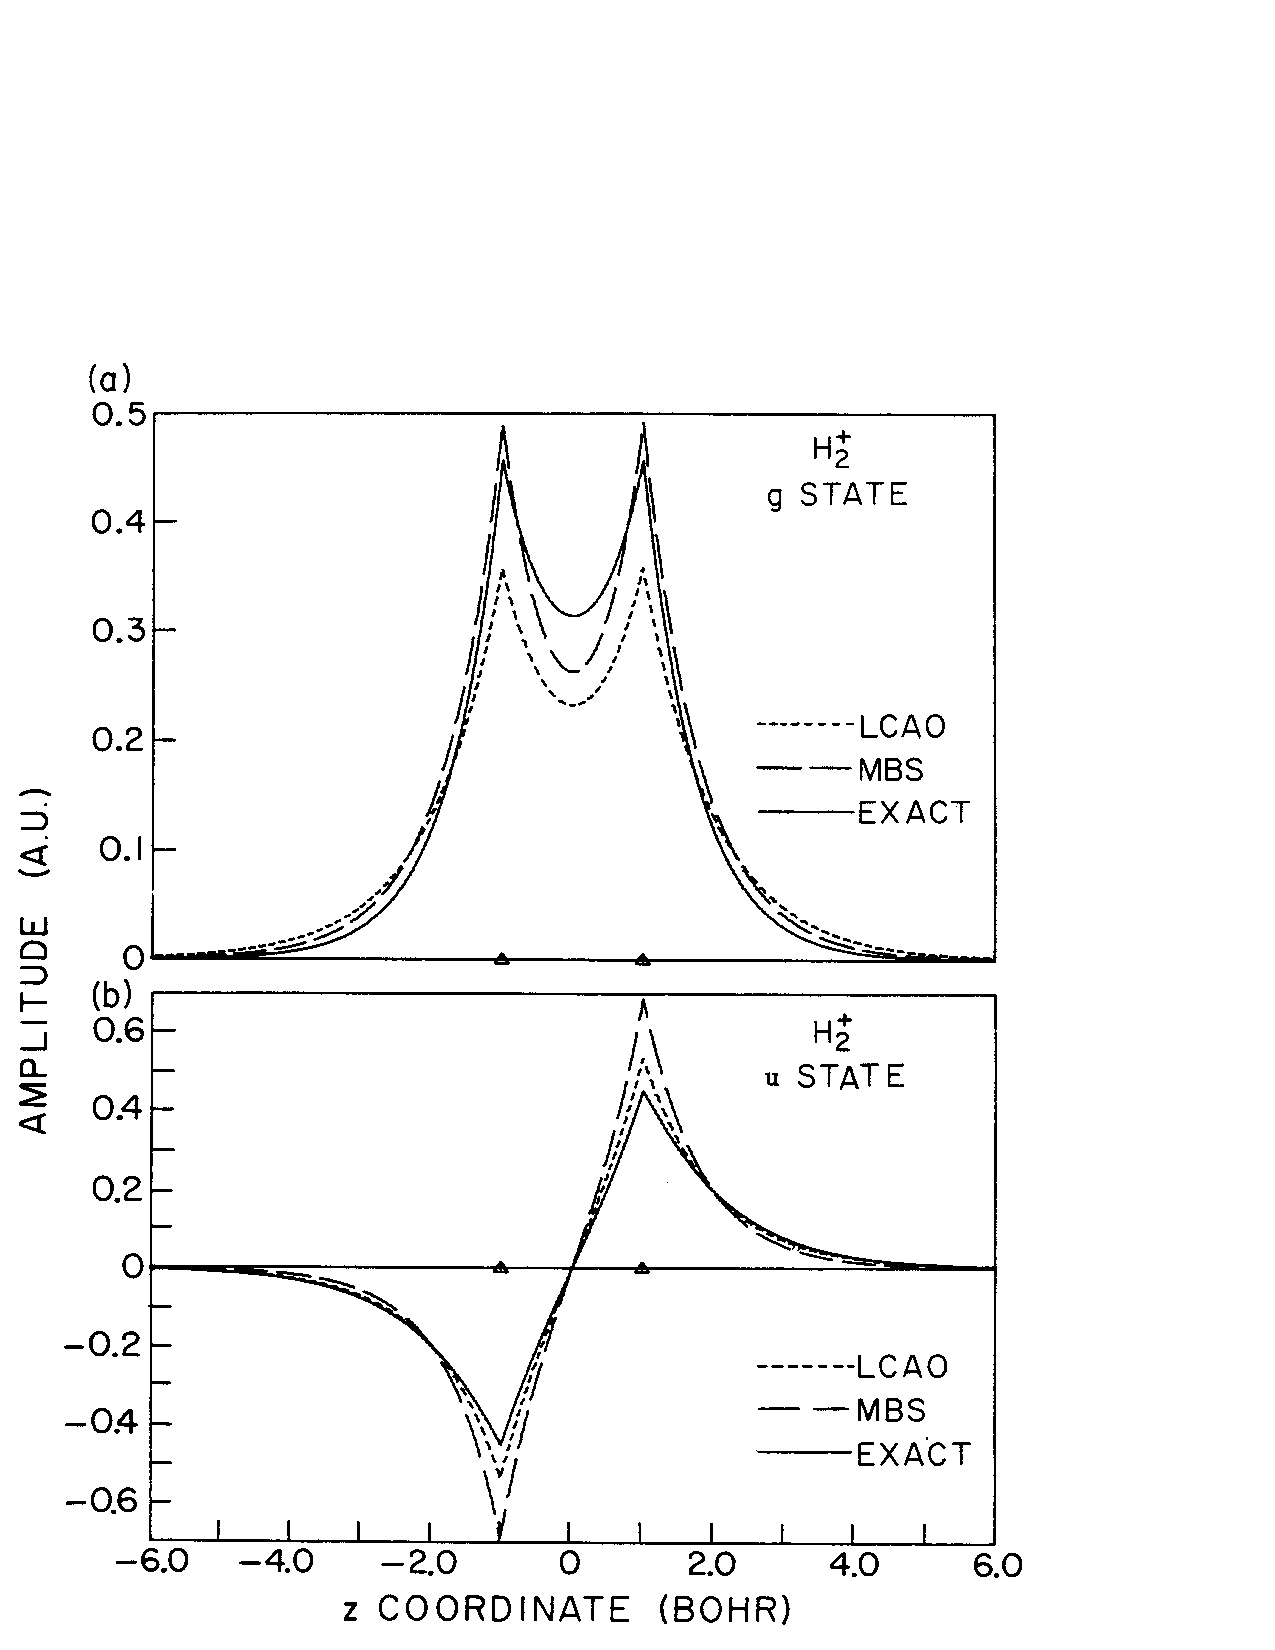
\includegraphics[scale=0.75]{fig3-03} 
\caption{The wavefunctions of H$^+_2$ at $R = 2.0a_0$.}
\label{fig3-04}
\end{figure}

\noindent
The MBS description leads to reasonably good densities near the nuclei
but too low a density in the bond region. Thus, with MBS the shape of
the wavefunction is not well described.

In the $u$ state, the LCAO
wavefunction is in much better agreement with the exact wavefunction
than is the MBS wavefunction. 

In Figure \ref{fig3-05}, we compare the LCAO and MBS wavefunctions as
a function of $R$, finding that the LCAO description does reasonably
well for $R > 4\ a_0$.  Note the large difference in the behavior of the
$g$ and $u$ states for small $R$.  These differences were also
manifest in the optimum exponents of Figure \ref{fig3-02}.

\begin{figure}
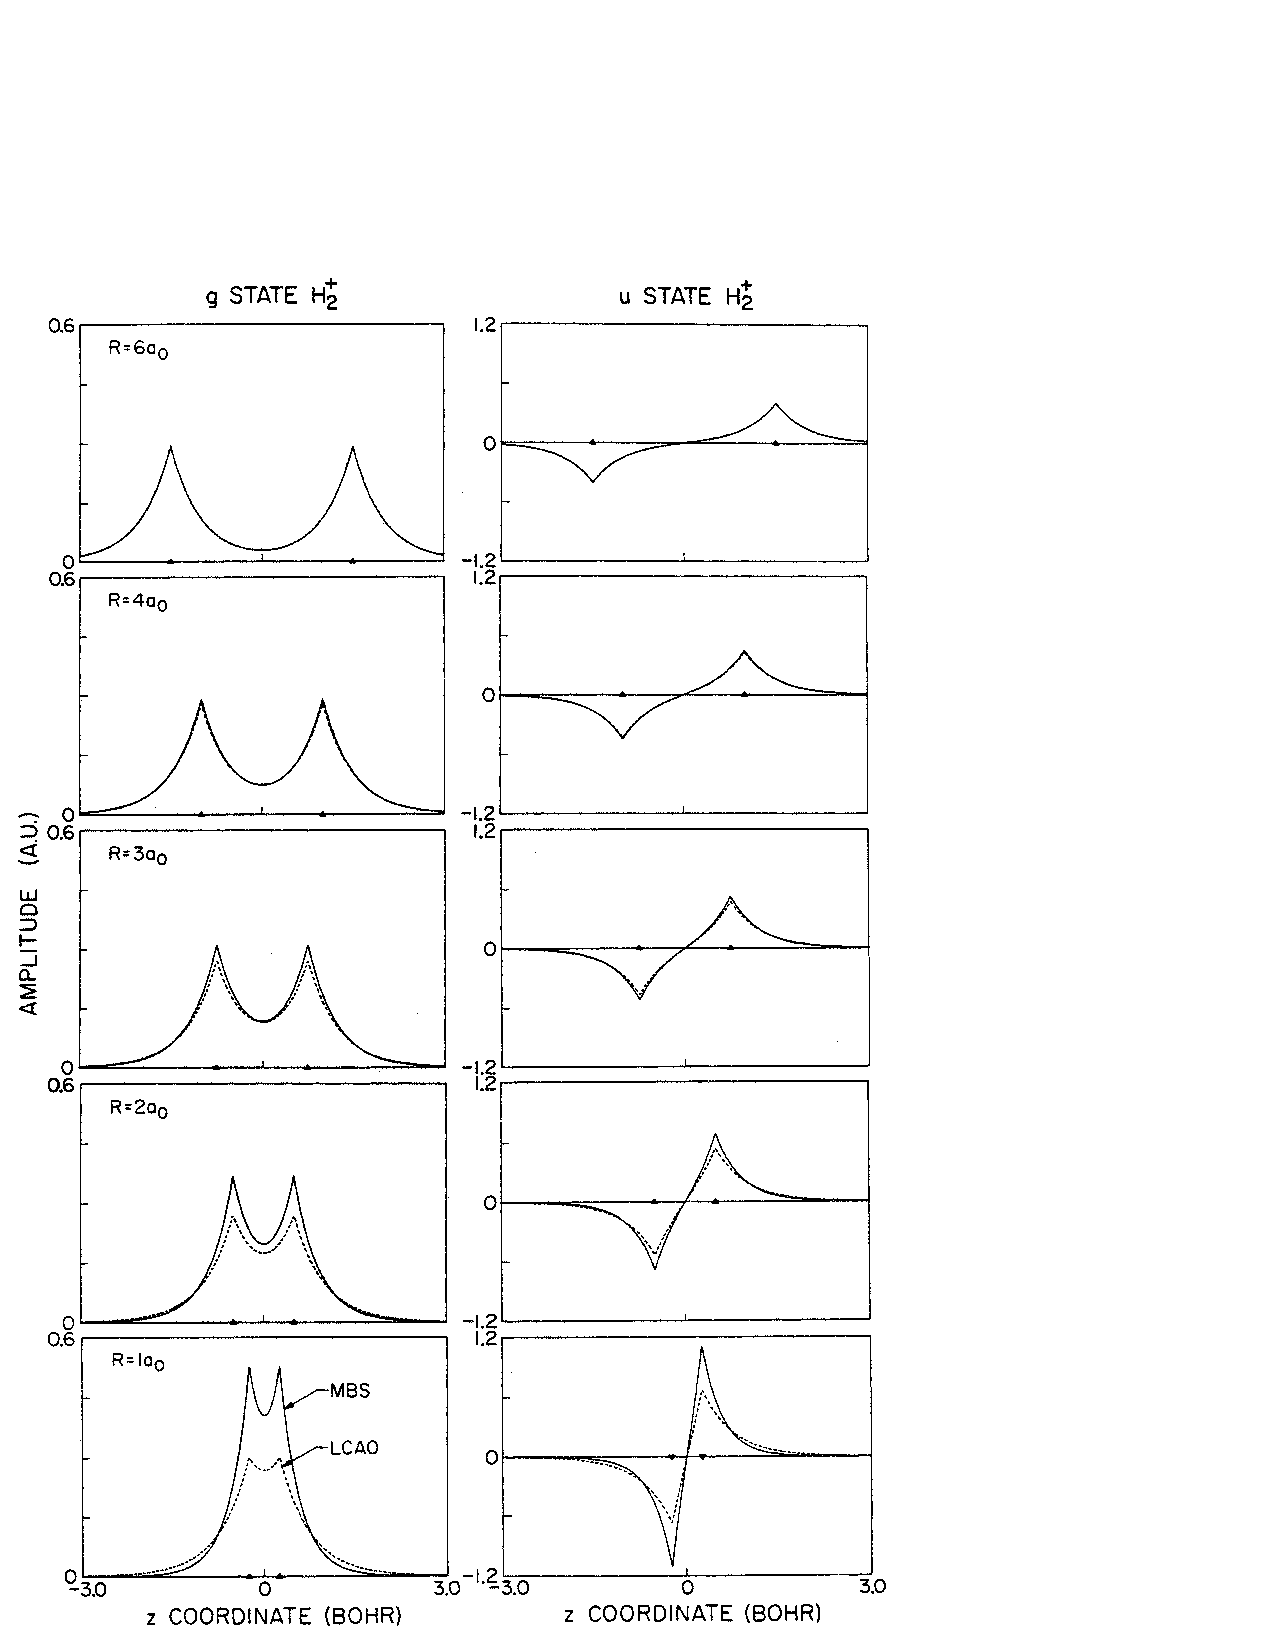
\includegraphics[scale=0.75]{fig3-04}
\caption{Amplitudes of the LCAO (dashed) and MBS (solid) wave
functions for (a) the $g$ state and (b) the $u$ state of H$^+_2$}
\label{fig3-05}
\end{figure}

\section{More on the Chemical Bond}

In Chapter 2 we analyzed the bond of H$^+_2$ in terms of the linear
combination of atomic orbitals description.  Now we will re-examine
the bond using more accurate wavefunctions.  With more accurate
wavefunctions, we still find that the exchange energy $E^x$ (more
specifically the exchange kinetic energy $T^x$ part of $E^x$) is
responsible for the bonding or antibonding of the $g$ and $u$ states
of H$^+_2$.  On the other hand, partitioning the energy into the total
potential energy ($V$) and the total kinetic, energy ($T$) we find
that neither can be solely responsible for bonding.

\subsection{The Classical and Exchange Energies}

Defining the classical and exchange terms, just as in Chapter 2,
\begin{equation}
E = E^{cl} + E^x
\label{chap3-eqno23}
\end{equation}
and
\begin{equation}
E^{cl} = \langle \chi_\ell \vert H \vert \chi_\ell \rangle
\end{equation}
but using the MBS wavefunctions, we obtain the results 
of Figure \ref{fig3-06}.

\begin{figure}
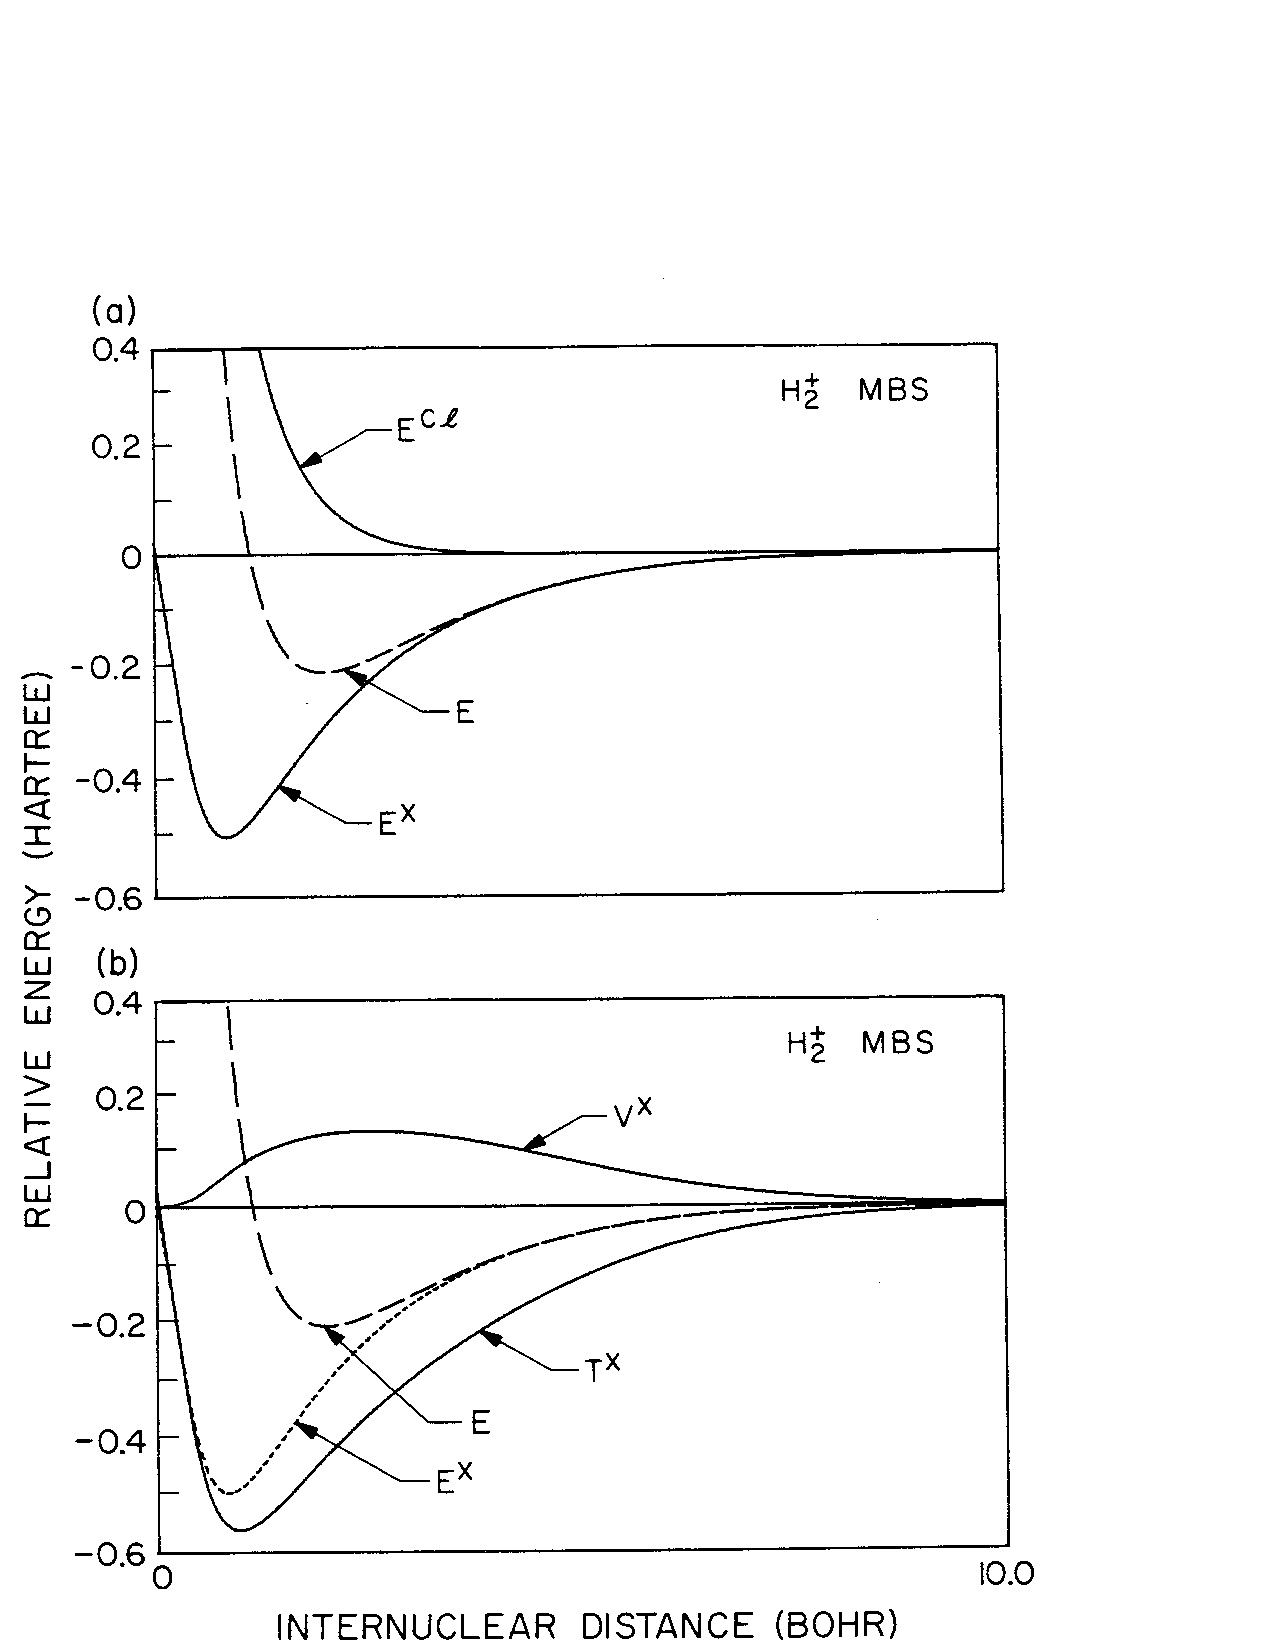
\includegraphics[scale=0.75]{fig3-05}
\caption{(a) The total energy, $E$, and the 
components $E^{cl}$ and $E^x$ for the MBS wavefunction
of the $g$ state of H$^+_2$. (b) The $T^x$ and $V^x$ components of
$E^x$ is shown.  All quantities are relative to $R = \infty$.}
\label{fig3-06}
\end{figure}

\noindent
Thus the exchange energy dominates the bonding just as for the linear 
combination of atomic orbitals wavefunction. Partitioning the $E^x$ 
into potential and kinetic parts, $V^x$ and $T^x$,
\begin{equation}
E^x = V^x + T^x
\end{equation}
as in Figure \ref{fig3-06}, we see that $T^x$ favors bond formation,
while $V^x$ opposes it, just as for the LCAO wavefunction.

Thus, in terms of the classical and exchange quantities, the linear
combination of atomic orbitals and MBS descriptions are quite
similar. In both cases, it is the large decrease in $T^x$ that is
responsible for bond formation. Just as discussed in Chapter 2, $T^x$
is large and negative because the atomic orbitals are contragradient
in the region between the nuclei. In particular, the $T^x$ is similar
in character for the LCAO and MBS descriptions.  With $\zeta > 1$ the
gradients get larger and favor a smaller $R$ so that the differences
in $T^x$ for the LCAO and MBS
descriptions are easily understood.

\subsubsection{An Ambiguity}

There is a flaw with this procedure of decomposing the energy into 
classical and exchange parts. Adding a second basis function on each 
center, say $\chi_{2\ell}$ and $\chi_{2r}$, and optimizing the coefficients, 
leads to
\begin{equation}
\Phi_g = C_1 \left( \chi_{1\ell} + \chi_{1r} \right) + C_2 \left( 
\chi_{2\ell} + \chi_{2r} \right)
\end{equation}
and adding additional functions, we ultimately obtain the exact 
wavefunction in the form
\begin{equation}
\Phi_g = \sum^{\infty}_{k=1} C_k \left( \chi_{k\ell} + \chi_{kr} \right) .
\end{equation}
Thus, we can define optimum left and right orbitals as
\begin{equation}
\chi_\ell = \sum_{k} C_k \chi_{k\ell}
\label{chap3-eqno24a}
\end{equation}
\begin{equation}
\chi_r = \sum_{k} C_k \chi_{kr}
\label{chap3-eqno24b}
\end{equation}
and obtain an exchange energy for the exact wavefunction.  The problem
is that for the exact wavefunction there is not a unique choice for
the left and right functions $\chi_\ell$ and $\chi_r$.  As a result,
there is some ambiguity in the exchange energy for the exact
wavefunction.  On the other hand, with optimized basis functions only
a few functions (say, two $s$ and one $p_z$ on each center) lead to
quite accurate descriptions but with no ambiguity in the decomposition
(\ref{chap3-eqno24a})--(\ref{chap3-eqno24b}).


\subsection{Potential and Kinetic Energies}

Rather than the partition (\ref{chap3-eqno23}) of the energy into
classical and exchange terms, it has been much more common to
partition the energy into total potential energy, $V$, and total
kinetic energy, $T$,
\begin{equation}
E = T + V
\label{chap3-eqno25}
\end{equation}
This partition mixes up the things characteristic of
bonding with other quantities that are nearly independent of bonding
with the result that neither quantity, $T$ or $V$, consistently
contains the bonding stuff.  A good illustration of this is to compare
the quantities for the LCAO and MBS
wavefunctions of H$^+_2$.  As shown earlier, the classical and
exchange energies behave very similarly for these two cases.  However,
as shown in Figure \ref{fig3-07}, the behavior of $T$ and $V$ for the
LCAO and MBS wavefunctions is
markedly different.

\begin{figure}
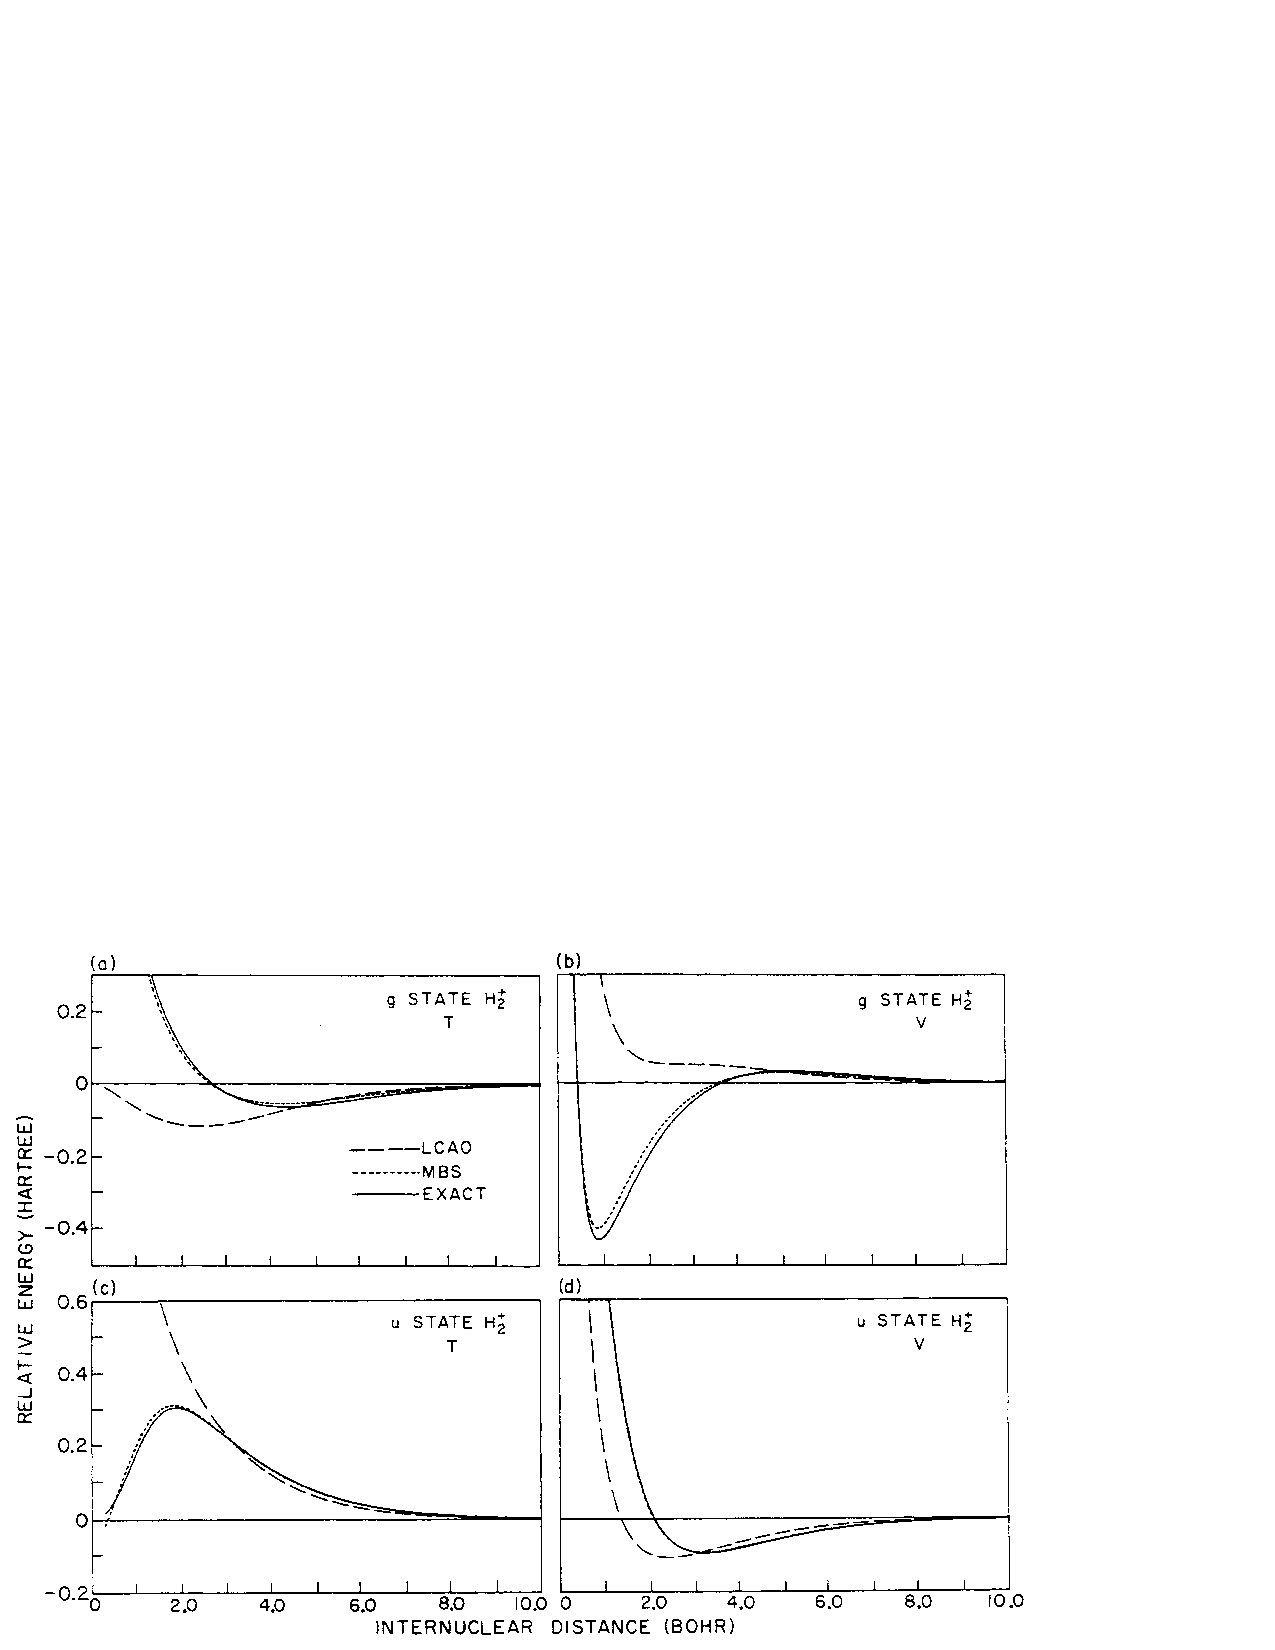
\includegraphics[scale=0.75]{fig3-06}
\caption{The kinetic and total potential energies for (a,b) the $g$ 
state, and (c,d) the $u$ state of H$^+_2$.  All quantities
are relative to the value for $R = \infty$.}
\label{fig3-07}
\end{figure}

Thus, for LCAO the $T(R)$ is always lower than $T(\infty)$, while
$V(R)$ is always higher than $V(\infty)$.  This might suggest that it
is kinetic energy that is responsible for the bond. However, for the
MBS wavefunction $T(R)$ is below $T(\infty)$ only for $R > 2.7\ a_0$.
Thus, at $R_e = 2\ a_0$, $T(R) > T(\infty)$ and it would be ludicrous
to assume that the total kinetic energy is the quantity dominating
bonding.  On the other hand, in the MBS wavefunction, $V(R) >
V(\infty)$ for $R = 3.5\ a_0$.  Thus, although $V(R)$ dominates the
bond at $R_e$, it opposes bond formation for $R < 3.5\ a_0$.
Furthermore, for the LCAO, $V(R)$ opposes bonding for all $R$.

Such difficulties show that (\ref{chap3-eqno25}) is not a useful
partition of the energy. The key indication of this is that although
the total energy changes monotomically from $R = \infty$ to $R_e$, the
$V$ and $T$ for the MBS and exact wavefunctions are not monotonic,
each dominating the energy over different regions. Hence, neither can
be uniquely responsible for bonding.

Occasionally, usually in the analysis of rotational and conformational barriers
in polyatomic molecules, energy curves are analyzed by partitioning 
the $V$ into various parts
\begin{equation}
V = V^{en} + V^{nn} + V^{ee}
\end{equation}
where $ee$ denotes electron-electron repulsion, $en$ denotes
electron-nuclear attraction, and $nn$ denotes nuclear-nuclear
repulsion terms, $ee$ is not present for H$^+_2$. As shown in Figure
\ref{fig3-08}, each term is monotomic, with $V^{en}$ decreasing with
$R$.  One might conclude from this that it is $V^{en}$ that is
responsible for bond formation.  However, as seen from Figure
\ref{fig3-08}(b), the $V^{en}$ and $V^{nn}$ are also monotonic for the
$u$ state and, again $V^{en}$ decreases with $R$, but this state is
repulsive. Thus, despite similar $V^{en}$ and $V^{nn}$ for $g$ and $u$
we obtain radically different potential curves.  Thus, $V^{en}$ is
dominated by quantities other than those responsible for bond
formation.


\begin{figure}
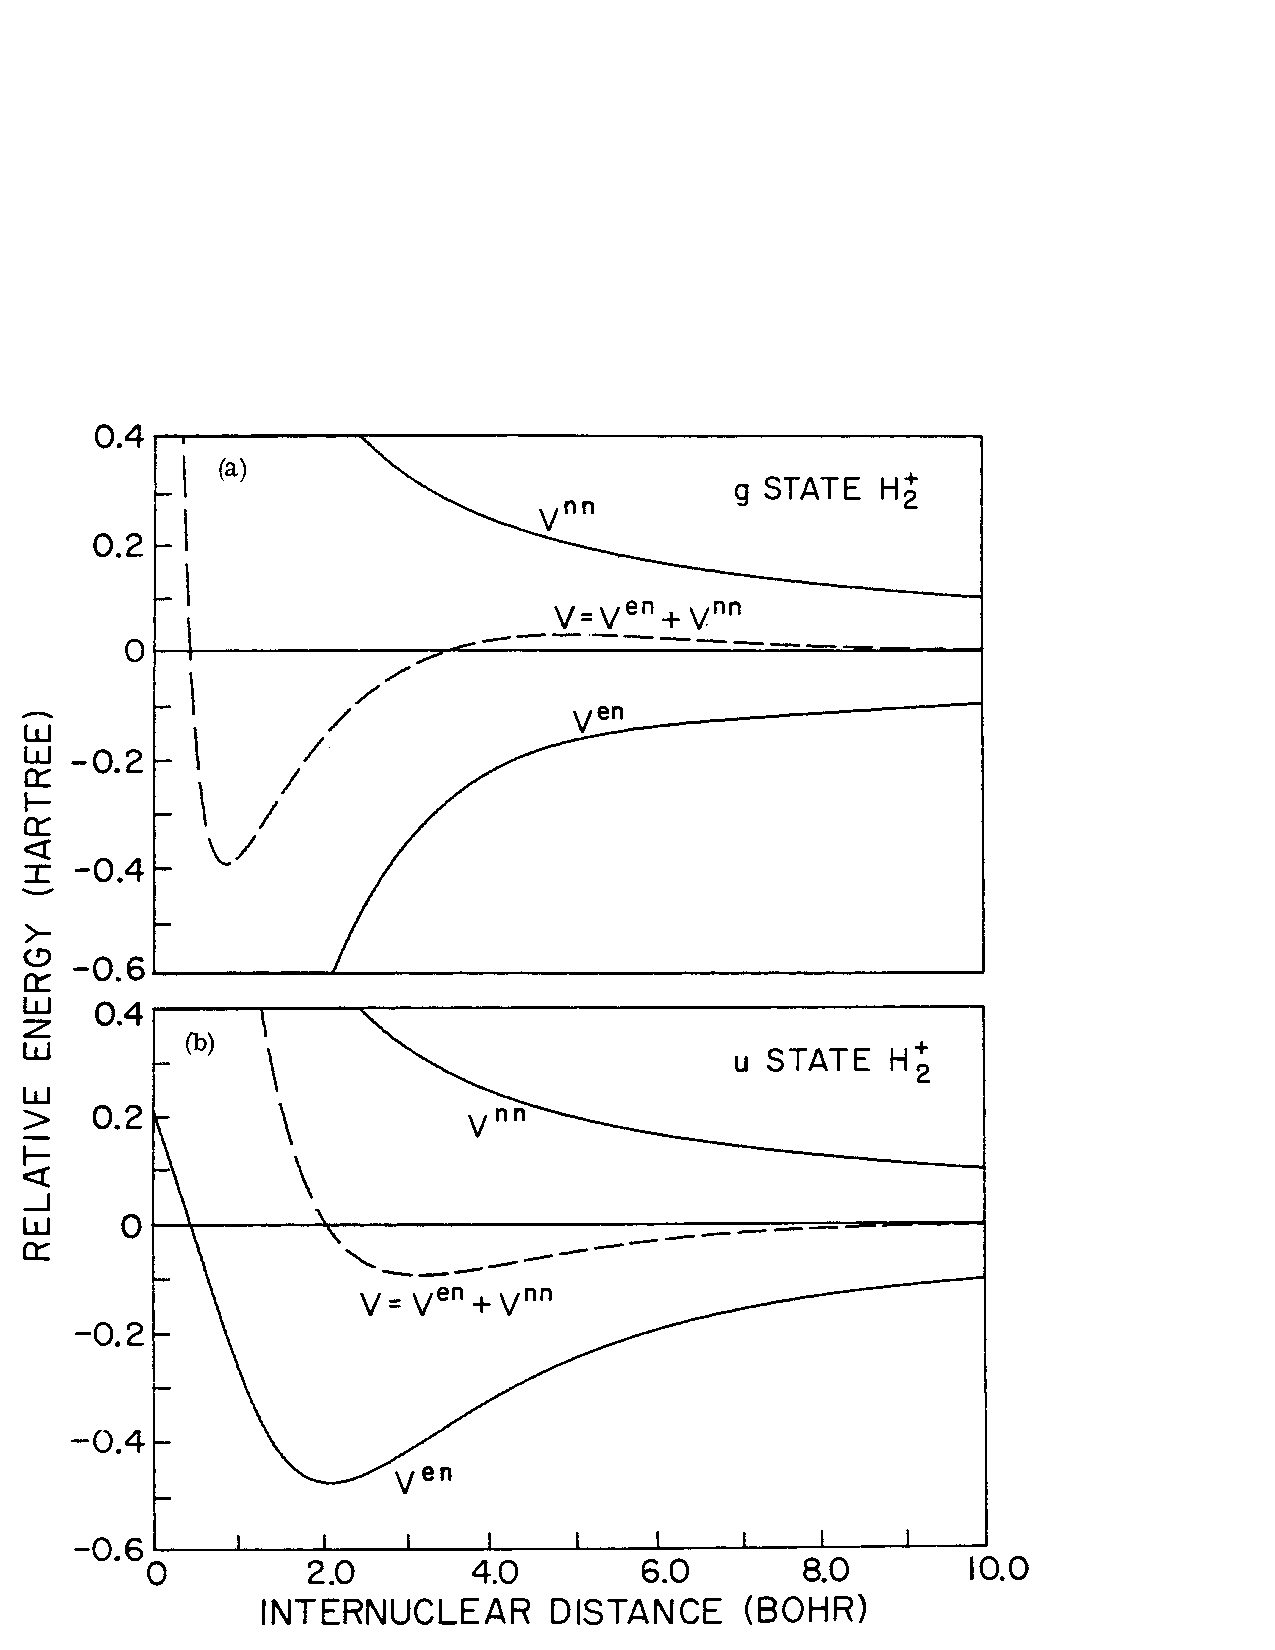
\includegraphics[scale=0.75]{fig3-07}
\caption{The total potential energy, $V$, and the partition 
into $V^{nn}$ and $V^{en}$ for (a) the $g$ state and
(b) the $u$ state of H$^+_2$, exact wavefunctions is shown. All
quantities are relative to the value for $R = \infty$.}
\label{fig3-08}
\end{figure}

\section{Overview of Theoretical Methods}

This course focuses primarily on \emph{qualitative} ideas of chemical
bonding rather than particular theoretical methods. However,
familiarity with the theoretical methods is important for discussing
qualitative ideas and hence, we will outline these methods.

\subsection{Basis Sets}

Several methods involve solving for the optimum shape of one-electron orbitals
$\varphi_i(r)$. The general procedure for carrying out such calculations,
involve selection of a basis set
\begin{equation}
\left\{ \chi_{\mu} ; \mu = 1 , \cdot \cdot \cdot , P 
\right\},
\label{chap3-eqno26}
\end{equation}
suitable for describing the optimum orbitals
\begin{equation}
\varphi_i ( r ) = \sum^{P}_{\mu = 1} C_{\mu i} \chi_{\mu} ( r ) .
\end{equation}
Here, the basis functions are fixed and hence, selection of the optimum 
coefficients
\begin{equation}
\left\{ C_{1i} , C_{2i} , \cdot \cdot \cdot , C_{Pi} \right\}
\end{equation}
serves to determine the orbital $\varphi_i(r)$.  This procedure is 
analogous to a Fourier expansion where harmonic functions (sines and 
cosines) are used as basis functions in (\ref{chap3-eqno26}).

For an exact description of the optimum orbital it is generally necessary 
to use an infinite number, a complete set, of basis functions.  However, 
for practical reasons we must use a finite set.  Indeed, from numerous 
studies of molecular wavefunctions, there are principles that can be used 
to select rather small basis sets that yield quite accurate wavefunctions.

In evaluating the wavefunctions and energies using a basis set, as in 
(\ref{chap3-eqno26}), we must evaluate integrals of the form
\begin{equation}
\langle \chi_{\mu} \vert h \vert \chi_{\nu} \rangle
\label{chap3-eqno27a}
\end{equation}
\begin{equation}
\langle \chi_{\mu} ( 1 ) \chi_{\nu} ( 2 ) \vert {1 \over r_{12}} 
\vert \chi_{\sigma} ( 1 ) \chi_{\eta} ( 2 ) \rangle ,
\label{chap3-eqno27b}
\end{equation}
where the functions may be centered at various regions of space. Thus, an
important criterion in selecting the basis is that the molecular integrals be
practicable to evaluate.  In order to obtain the best wavefunctions 
with the fewest basis functions, we want to choose the basis functions 
to have shapes characteristic of the eigenstates of the molecular systems.

For a Coulomb potential, i.e. the hydrogen atom, the eigenstates have the form
\begin{equation}
1s : e^{-Zr}
\end{equation}
\begin{equation}
2s : (r - \alpha ) e^{-{1 \over 2}Zr}
\end{equation}
\begin{equation}
2p_z : r \cos \theta e^{-{1 \over 2} Zr}
\end{equation}
\begin{equation}
2p_x : r \sin \theta \cos \varphi e^{-{1 \over 2} Zr}
\label{chap3-eqno28}
\end{equation}
\begin{equation}
2p_y : r \sin \theta \cos \varphi e^{-{1 \over 2} Zr}
\end{equation}
\begin{equation}
3s : \left( r^2 - \beta r + \alpha \right) e^{-{1 \over 2} Zr}
\end{equation}
\centerline{etc.}

\noindent
where normalization is ignored and the constants $\alpha$ and $\beta$
are unimportant to our considerations here.  In order to describe,
with finite number of basis functions, singular characteristics such
as the cusps occurring near the various nuclei, we should include in
our basis set functions having similar singular characteristics. Thus,
for a molecular system, we should use atomic functions like
(\ref{chap3-eqno28}) centered upon the various nuclei of the molecule.

The radial parts of the functions in (\ref{chap3-eqno28}) all can be
built from functions of the form
\begin{equation}
r^n e^{- \zeta r},
\label{chap3-eqno29}
\end{equation}
where various values of n and of the orbital exponents, $\zeta$, must
be allowed.  Functions of the form (\ref{chap3-eqno29}) are preferable
to the hydrogen atom orbitals (\ref{chap3-eqno28}), since
(\ref{chap3-eqno29}) is more convenient for evaluating the molecular
integrals. Combining functions of the form (\ref{chap3-eqno29}) with
appropriate angular functions, $Z_{lm}$ the real spherical harmonics,
leads to a convenient set of one-particle orbitals
\begin{equation}
r^n e^{- \zeta r} Z_{lm} \left( \theta , \varphi \right)
\label{chap3-eqno30}
\end{equation}
for use in atomic and molecular wavefunctions.  These functions
(\ref{chap3-eqno30}) are referred to as \emph{Slater functions}, or
\emph{Slater-type orbitals} (STO) in honor of an early exponent
\cite{chap3-ref5} of such functions.  We will use the term function
when referring to an arbitrary function as in a basis function, and
the term orbital when referring to a specific optimized orbitals as in
a HF or GVB orbital.  They are denoted as $1s$, $2s$, $2p$, etc., just
as for hydrogen atom orbitals.  The orbital exponent, $\zeta$, in
(\ref{chap3-eqno29}) is considered as an adjustable parameter and is
generally chosen as the optimum value for the particular molecule and
basis set of interest (rather than taken as $\zeta = Z/n$ as suggested
by (\ref{chap3-eqno28})).

For example, a good basis for describing the wavefunction for H$_2$ is
to use two ls Slater functions (denoted as $1s$ and $1s^{\prime}$) a
$2s$ Slater function, and a set of the $2P$ Slater functions, $2p_z$,
$2p_x$, and $2p_y$, on each center. The optimum exponents at $R =
1.4\ a_0$ are \cite{chap3-ref6}
\begin{eqnarray}
\zeta ( 1 s ) &= 0.965\\
\zeta ( 1 s^{\prime} ) &= 1.43\\
\zeta ( 2 s ) &= 1.16\\
\zeta ( 2 pz ) &= 1.87\\
\zeta (2 px ) &= \zeta ( 2py ) = 1.71
\end{eqnarray}

\noindent 
where the molecular axis is along $z$.  With this basis, the CI
wavefunction leads to an energy of $-1.16696$ h, at $R = 1.4a_0$,
99.4\% of the exact answer$^7$ $-1.17447$ h.  Note that the optimum
orbital exponents are significantly different from the values for the
free atom
\begin{equation}
\zeta_{1s} = 1.0
\end{equation}
\begin{equation}
\zeta_{2s} = 0.5
\end{equation}
\begin{equation}
\zeta_{2p} = 0. 5.
\end{equation}

The second type of basis functions, commonly used in molecular
calculations, are \emph{Gaussian functions} where the $e^{-\zeta r}$
of (\ref{chap3-eqno30}) is replaced by $e^{-\alpha r^2}$ and $n$ is
taken as $l$,
\begin{equation}
r^l e^{- \alpha r^2} Z_{lm} \left( \theta , \varphi \right)
\end{equation}
Although Gaussian functions have the wrong behavior as $r \rightarrow
0$, and as $r \rightarrow \infty$, they serve just as well as Slater
functions in describing the valence orbitals and the bonds of
molecules. The major advantage of Gaussian functions is that the
molecular integrals (\ref{chap3-eqno27a})--(\ref{chap3-eqno27b})
required for large molecules are much simpler, and less time
consuming, than for Slater functions.

Generally, basis sets are optimized for atoms.  If properly carried
out, the atomic basis sets supplemented by a few additional functions,
polarization functions, serve to provide very accurate descriptions of
the molecular wavefunctions.

\subsection{The HF Method}

\subsubsection{The Basic Equations}

In Chapter 2 we described the simple MO wavefunction of H$_2$ in
which the two-electron wavefunction is expressed as
\begin{equation}
\Phi ( 1 , 2 ) = \varphi ( 1 ) \chi ( 2 )
\label{chap3-eqno31}
\end{equation}
where $\varphi$ is the MO
\begin{equation}
\varphi = {( \chi_\ell + \chi_r ) \over \sqrt{2(1+S)}}
\end{equation}
and $\chi_\ell$ and $\chi_r$ are hydrogen orbitals centered on the two 
nuclei.  Now we will consider the case where $\varphi$ is allowed to be 
completely general.  Thus, if $\{ \chi_{\mu} \}$ is some basis set,
we write
\begin{equation}
\varphi = \sum_{\mu} C_{\mu} \chi_{\mu}
\label{chap3-eqno32}
\end{equation}
with the coefficients $\{ C_{\mu} \}$ chosen so that $\Phi$ in
(\ref{chap3-eqno31}) leads to the lowest possible energy.

The energy of (\ref{chap3-eqno31}) is
\begin{equation}
E = {\langle \Phi \vert H^{el} \vert \Phi \rangle \over \langle 
\Phi \vert \Phi \rangle} = 2 \langle \varphi \vert h \vert \varphi 
\rangle + J_{\varphi \varphi} + {1 \over R} ,
\label{chap3-eqno33}
\end{equation}
where
\begin{equation}
J_{\varphi \varphi} = ( \varphi \varphi \vert \varphi \varphi ) = \int
d^3 r_1 \varphi^* (1) \varphi (1) \int d^3 r_2 {\varphi^* (2)
  \varphi(2) \over r_{12}}
\end{equation}
and
\begin{equation}
\langle \varphi \vert \varphi \rangle = 1 .
\label{chap3-eqno34}
\end{equation}
Applying the variational principle to (\ref{chap3-eqno33})
\begin{equation}
{\partial E \over \partial C_{\mu}} = 0
\end{equation}
with the constraint (\ref{chap3-eqno34}), leads to
\begin{equation}
\langle \chi_{\mu} \vert \left( h + J_{\varphi} - \epsilon \right) \vert 
\varphi \rangle = 0
\label{chap3-eqno35}
\end{equation}
where $\epsilon$ is referred to as the orbital energy,
\begin{equation}
\epsilon = \langle \varphi \vert h \vert \varphi \rangle + J_{\varphi \varphi} 
,
\label{chap3-eqno36}
\end{equation}
and
\begin{equation}
J_{\varphi} ( r_1 ) = \int d^3 r_2 {\varphi^* (r_2) \varphi (r_2) \over r_{12}}
\end{equation}
is the electrostatic potential at point $r_1$ due to the charge 
density $\vert \varphi ( r_2 ) \vert^2$ integrated over all $r_2$.

Substituting (\ref{chap3-eqno32}) into (\ref{chap3-eqno35}) leads to
\begin{equation}
\sum^{P}_{\nu = 1} \left( H_{\mu \nu} - \epsilon S_{\mu \nu} \right) 
C_{\nu} = 0 ; \mu = 1 , 2 , \cdot \cdot \cdot , P.
\label{chap3-eqno37}
\end{equation}
where
\begin{equation}
H_{\mu \nu} = \langle \chi_{\mu} \vert \left( h + J_{\varphi} 
\right) \vert \chi_{\nu} \rangle
\label{chap3-eqno38a}
\end{equation}
\begin{equation}
S_{\mu \nu} = \langle \chi_{\mu} \vert \chi_{\nu}.
\label{chap3-eqno38b}
\end{equation}
In matrix notation, (\ref{chap3-eqno37}) is written as
\begin{equation}
\mathbf{HC} = \mathbf{SC} \epsilon .
\label{chap3-eqno39}
\end{equation}
Since
\begin{equation}
\langle \chi_{\mu} \vert J_{\varphi} \vert \chi_{\nu} \rangle = 
\sum_{\sigma , \eta} C_{\sigma} C_{\eta} \langle \chi_{\mu} 
\chi_{\sigma} \vert {1 \over r_{12}} \vert \chi_{\nu} \chi_{\eta} 
\rangle ,
\end{equation}
$H_{\mu \nu}$ is a function of the unknowns $\{ C_{\mu} \}$ and
(\ref{chap3-eqno37}) is nonlinear. Since the basis functions $\{
\chi_{\mu} \}$ are known, all integrals in
(\ref{chap3-eqno38a})--(\ref{chap3-eqno38b}) can be evaluated just
once so that (\ref{chap3-eqno39}) becomes a nonlinear algebraic
equation.

In order for the variational condition of (\ref{chap3-eqno35}) to be
satisfied for all $\chi_{\mu}$ of a complete set, the function $(h +
J_{\varphi} - \epsilon)\varphi$ must be zero.  That is, the
differential equation
\begin{equation}
( h + J_{\varphi} ) \varphi = \epsilon \varphi
\label{chap3-eqno40}
\end{equation}
or (for H$_2$)
\begin{equation}
\left( - {1 \over 2} \nabla ^2 - {1 \over r_a} - {1 \over r_b} + 
J_{\varphi} \right) \varphi = \epsilon \varphi
\end{equation}
must be satisfied in order that $\varphi$ be a completely optimum function. The
resulting optimum wavefunction of (\ref{chap3-eqno31}) is called the HF 
wavefunction, the optimum orbital of (\ref{chap3-eqno40}) is called the HF
orbitals, and this whole approach is called the HF method, all 
in honor of the Englishman D. R. Hartree, and the Russian V. Fock
(sometimes Fok) who first developed it. 

\subsubsection{Solution of the HF Equations}

The differential equation (\ref{chap3-eqno40}) is not linear in
$\varphi$ since $J_{\varphi}$ depends upon $\varphi$.  The usual
approach to solving (\ref{chap3-eqno40}) is the iterative method in
which we guess the orbital, $\varphi_0$, evaluate $J_{\varphi_0}$, and
solve the linear equation
\begin{equation}
( h + J_{\varphi_0} ) \varphi_1 = \epsilon \varphi_1
\end{equation}
for a one orbital $\varphi_1$.  Then $\varphi_1$ is used to evaluate a new 
$J_{\varphi_1}$ and
\begin{equation}
( h + J_{\varphi_1} ) \varphi_2 = \epsilon \varphi_2
\end{equation}
is solved for a new orbitals.  This process is continued until it 
converges, that is, until
\begin{equation}
\varphi_{I+1} \approx \Phi_I .
\end{equation}

For atoms, the HF equation (\ref{chap3-eqno40}) can be reduced to
one-dimension and solved numerically.  However, for molecules the only
practial procedure is to use a finite basis set and to solve the
resulting matrix equations (\ref{chap3-eqno37}) and
(\ref{chap3-eqno39}).  These are also solved iteratively.  One guesses
the coefficients $\{C^0_{\mu} \}$ and evaluates the $H_{\mu \nu}$ of
(\ref{chap3-eqno38a})--(\ref{chap3-eqno38b}).  With $H_{\mu \nu}$
fixed, the matrix equations (\ref{chap3-eqno37}) and
(\ref{chap3-eqno39}) are linear and easy to solve for a new set of
coefficients $\{ C^{\prime}_{\mu} \}$. This process is continued until
it converges.

By solving the matrix HF equations
(\ref{chap3-eqno38a})--(\ref{chap3-eqno38b}) and (\ref{chap3-eqno39})
for larger and larger basis sets, one can in the limit approach the
results of solving the numerical equation (\ref{chap3-eqno40}).  Indeed,
by proper choice of the basis functions it is possible to obtain very
accurate solutions for very small $P$, e.g., $P = 2$ for He, and $P =
6$ for H$_2$.

\subsubsection{Historical Note}

Before real quantum mechanics, i.e., the work of Schr\"odinger, Heisenberg, 
and their contemporaries in 1925 and 1926, physicists and chemists were 
attempting to understand the structure of atoms, and molecules, on the basis 
of a many-electron Bohr atom.  The idea was that each electron moved along 
a different Bohr orbit, experiencing electrostatic interactions due to all 
the other electrons but satisfying various, postulated, rules in order to 
obtain agreement with the periodic properties of the elements.

Hartree suggested \cite{chap3-ref8} approximating this problem by
assuming that the average interaction with the other electrons leads
to a new potential that is a function only of the distance from the
nucleus.  He then tried to determine the form of $V(r)$, same $V(r)$
for all orbitals, by fitting to the experimental energies of the
orbits of various electrons, e.g., from X-ray data.

After quantum mechanics, Hartree realized that he could convert this
idea into quantum mechanics and actually solve for the potential and
orbital.  He thus started directly with (\ref{chap3-eqno40}), and its
generalization for more electrons, and began solving for atomic
wavefunctions (\cite{chap3-ref9}). These equations are called the
Hartree equations.  Hartree, a properly modest English gentleman,
continued to call them the self-consistent field, SCF, equations.

In 1930, Slater pointed out \cite{chap3-ref10} that Hartree's equations
could be derived using the variational principle, thus putting
Hartree's {\it ad hoc} approach on a more fundamental basis.  Slater
also pointed out that for many-electron atoms, there are additional
terms, we call them exchange terms, that should be in the
wavefunction, from the Pauli principle, see Chapter 4.  However,
Slater showed that these terms were of the same size as the intrinsic,
correlation, errors in the Haxtree approach and did not pursue them
further.

Also in 1930, V. Fock \cite{chap3-ref11} included the Pauli principle
and derived the corresponding variational equations obtaining
Hartree's equations, but with additional exchange terms. These
equations are now known as the HF equations.  Hartree referred to them
as self-consistent field with exchange.

The approach of using a finite basis set for obtaining HF
wavefunctions, rather than solving numerically, via Hartree, is
sometimes called HF Roothaan, in honor of the early leader in the
development and application of this procedure \cite{chap3-ref12}.  We
will make no such distinctions, although Roothaan's paper is amazingly
complete and he is rightfully credited with the development of the
basis set expansion (BSE) approach.  An early application of BSE was
by Coulson \cite{chap3-ref13} who concluded that the basis set
expansion was not practical and that self-consistent field orbitals
would not prove to be very useful for molecular structures.
Basically, Coulson showed that the same effort required to obtain an
accurate HF wavefunction would, if applied to other forms of the
wavefunction, with electron correlation, yield far better energies.
The point missed by Coulson is that for larger systems, these other
methods quickly become much more cumbersome and expensive than HF.
Roothaan's work came at just the right time.  Application of the basis
set expansion approach for larger molecules depends upon electronic
computers, the development of which was just starting in 1951.

\subsubsection{Interpretation, Correlation and Koopmans' Theorem}

The variational condition of (\ref{chap3-eqno40}) has the form of a
Schr\"odinger equation for a particle moving in the potential
\begin{equation}
V = - {1 \over r_a} - {1 \over r_b}  + J_{\varphi}
\end{equation}
assuming for the moment, H$_2$.  This is just the classical potential
that would be obtained if the second electron were replaced by its
classical potential, $J_{\varphi}$.  Thus, the HF orbital is the
eigenstate of the motion of an electron in the \emph{average}
potential due to the other electron.  Indeed, Hartree originally
derived his equations from just such classical considerations. In the
above derivation however, we applied the variational principle and
found that the best possible orbital satisfies such an equation.

Of course, in the real molecule the electron motions will be such as
to keep $1/r_{12}$ as small as possible, and $1/r_a$ and $1/r_b$ as
big as possible, while also minimizing the kinetic energy.  Thus, at
instants for which one of the electrons happens to be close to the
left nucleus, we expect that the other electron will tend to be near
the right nucleus. Such instantaneous correlations in the motion of
the electrons are ignored in the HF wavefunction.  Both electrons move
in the same orbital independently of the instantaneous position of the
other electron.  Hence, the error in the HF wavefunction is called the
\emph{correlation error}.

The energy $\epsilon$ in (\ref{chap3-eqno40}) is called the
\emph{orbital energy}.  From (\ref{chap3-eqno36}) it has the value
\begin{equation}
\epsilon = \langle \varphi \vert h \vert \varphi \rangle + J_{\varphi \varphi} = 
E_2 - E_1
\end{equation}
where
\begin{equation}
E_2 = 2 \langle \varphi \vert h \vert \varphi \rangle + J_{\varphi \varphi}
\end{equation}
is the energy of the two electron system with both electrons in $\varphi$, while
\begin{equation}
E_1 = \langle \varphi \vert h \vert \varphi \rangle
\end{equation}
is the energy with only one electron in $\varphi$. Thus, $\epsilon$ is
just the negative of the \emph{ionization potential}.  There are two
approximations here.  One is using the HF energy for the two-electron
molecule, leading to too high an energy for the two-electron system.
The other error is in describing the ion with the optimum orbital
$\varphi$ found for the two-electron molecule, leading to too large an
energy for the ion.  These errors often tend to cancel yielding
ionization potentials within about 10\% of the exact value. This
approximation, the first \cite{chap3-ref9} of using the orbital energy
to approximate the ionization potential is often called \emph{Koopmans
theorem}.  Note that there is an ess at the end of this name, and the
Dutch oo sounds about like our long o.  Although not strictly the
theorem that Koopmans proved,$^{14}$ we will also refer to this
approximation as Koopmans theorem.  Shortly after this work, Koopmans
switched to economics.  Koopmans is on the Economic faculty at Yale,
and in 1975 won a Nobel Prize for his work in optimization theory of
economics.

\subsection{The GVB Method}

In Chapter 2 we described the simple VB wavefunctions of
H$_2$, in which the two-electron wavefunction is expressed as
\begin{equation}
\Phi (1, 2) = ( \chi_\ell \chi_r + \chi_r \chi_\ell ),
\label{chap3-eqno41}
\end{equation}
where $\chi_\ell$ and $\chi_r$ are atomic orbitals.

We will not consider wavefunctions of the VB form
\begin{equation}
\Phi (1, 2) = \varphi_a \varphi_b + \varphi_b \varphi_a
\label{chap3-eqno42}
\end{equation}
but where the orbitals $\varphi_a$ and $\varphi_b$ are allowed to be completely 
general.  To obtain the best such orbitals, we will apply the variational 
principle, requiring the orbitals to lead to the lowest possible energy.  The 
optimum orbitals are called the GVB orbitals and the 
resulting wavefunction is called the \emph{GVB wavefunction}.

\subsubsection{The Basic Equations}

The energy of the GVB wavefunction (\ref{chap3-eqno42}) is
\begin{equation}
E = {N \over D} + {1 \over R}
\end{equation}
where
\begin{equation}
N = \left[ \langle a \vert h \vert a \rangle + \langle b \vert h \vert 
b \rangle + J_{ab} \right] + \left[ 2 \langle a \vert h \vert b 
\rangle S_{ab} + K_{ab} \right]
\end{equation}
\begin{equation}
D = 1 + S^2_{ab}
\end{equation}
\begin{equation}
S_{ab} = \langle a \vert b \rangle .
\end{equation}
Here, and in most of the following, we will use orbital subscripts,
e.g., $a$ and $b$, to denote orbitals (e.g., $\varphi_a$ and
$\varphi_b$, respectively).  Just as in the previous section, we will
consider that $\varphi_a$ and $\varphi_b$ are expanded in a basis $\{
\chi_{\mu} \}$
\begin{equation}
\varphi_a = \sum_{\mu} \chi_{\mu} C_{\mu a}
\label{chap3-eqno43a}
\end{equation}
and
\begin{equation}
\varphi_b = \sum_{\mu} \chi_{\mu} C_{\mu b}
\label{chap3-eqno43b}
\end{equation}
and require that
\begin{equation}
{\partial E \over \partial C_{\mu a}} = 0
\end{equation}
\begin{equation}
{\partial E \over \partial C_{\mu b}} = 0 .
\end{equation}
This condition leads to
\begin{equation}
\langle \chi_{\mu} \vert \left( H^a - \epsilon_a \right) \vert 
\varphi_a \rangle = 0,
\label{chap3-eqno44}
\end{equation}
where
\begin{equation}
\epsilon_a = E - \langle b \vert h \vert b \rangle
\end{equation}
and $H^a$ is an operator taking care of all other terms.  The form 
of $H^a$ is
\begin{equation}
H^a = ( h + J_b + K_b) + P_ bh + h P_b - EP_b
\end{equation}
where $P_b = \vert b > < b \vert$ is a projection operator.
However, the explicit form is of no importance here.  To solve
(\ref{chap3-eqno44}), we expand $\varphi_a$ with (\ref{chap3-eqno43a})--
(\ref{chap3-eqno43b}) leading to
\begin{equation}
\sum_{\nu} \langle \chi_{\mu} \vert \left( H^a - \epsilon_a \right) 
\vert \chi_{\nu} \rangle C_{\nu a} = 0 ,
\end{equation}
which, in matrix notation, is
\begin{equation}
\mathbf{H}^a \mathbf{C}_a = \epsilon_a \mathbf{SC}_a 
,
\label{chap3-eqno45}
\end{equation}
where the elements of the $\mathbf{H}^a$ and $\mathbf{S}$ matrices are
\begin{eqnarray}
H^a_{\mu \nu} &=& \langle \chi_{\mu} \vert H^a \vert \chi_{\nu} 
\rangle\\
&=& \langle \chi_{\mu} \vert \left( h + J_b + K_b \right) 
\vert \chi_{\nu} \rangle + \langle \chi_{\mu} \vert b \rangle \langle 
b \vert h \vert \chi_{\nu} \rangle + \langle \chi_{\mu} \vert h \vert 
b \rangle \langle b \vert \chi_{\nu} \rangle - E \langle \chi_{\mu} 
\vert b \rangle \langle b \vert \chi_{\nu} \rangle
\label{chap3-eqno46}
\end{eqnarray}
and
\begin{equation}
S_{\mu \nu} = \langle \chi_{\mu} \vert \chi_{\nu} \rangle .
\end{equation}

For the HF wavefunction, the corresponding matrix is
\begin{equation}
H^{HF}_{\mu \nu} = \langle \chi_{\mu} \vert \left( h + J_b \right) 
\vert \chi_{\nu} \rangle
\end{equation}
The presence of the second (exchange) term in the wavefunction
(\ref{chap3-eqno42}) leads to the other terms in (\ref{chap3-eqno46}).  Of
these additional terms, only the $K_b$ term would be present if the
orbitals $\varphi_a$ and $\varphi_b$ were orthogonal.

Equation (\ref{chap3-eqno45}) is the condition for orbital $\varphi_a$
to be optimum, there is a similar equation
\begin{equation}
\mathbf{H}^b \mathbf{C}_b = \epsilon_b \mathbf{SC}_b
\end{equation}
to solve for the optimum orbital $\varphi_b$.  Thus, in the GVB
method, we must solve self-consistently for \emph{two} orbitals,
whereas in the HF method we have just one orbital, and hence, one
equation to solve.  Otherwise both involve similar computational
procedures.

As shown in Figure \ref{fig3-09}, the GVB orbital
of H$_2$ corresponds closely to the VB orbital.

\begin{figure}
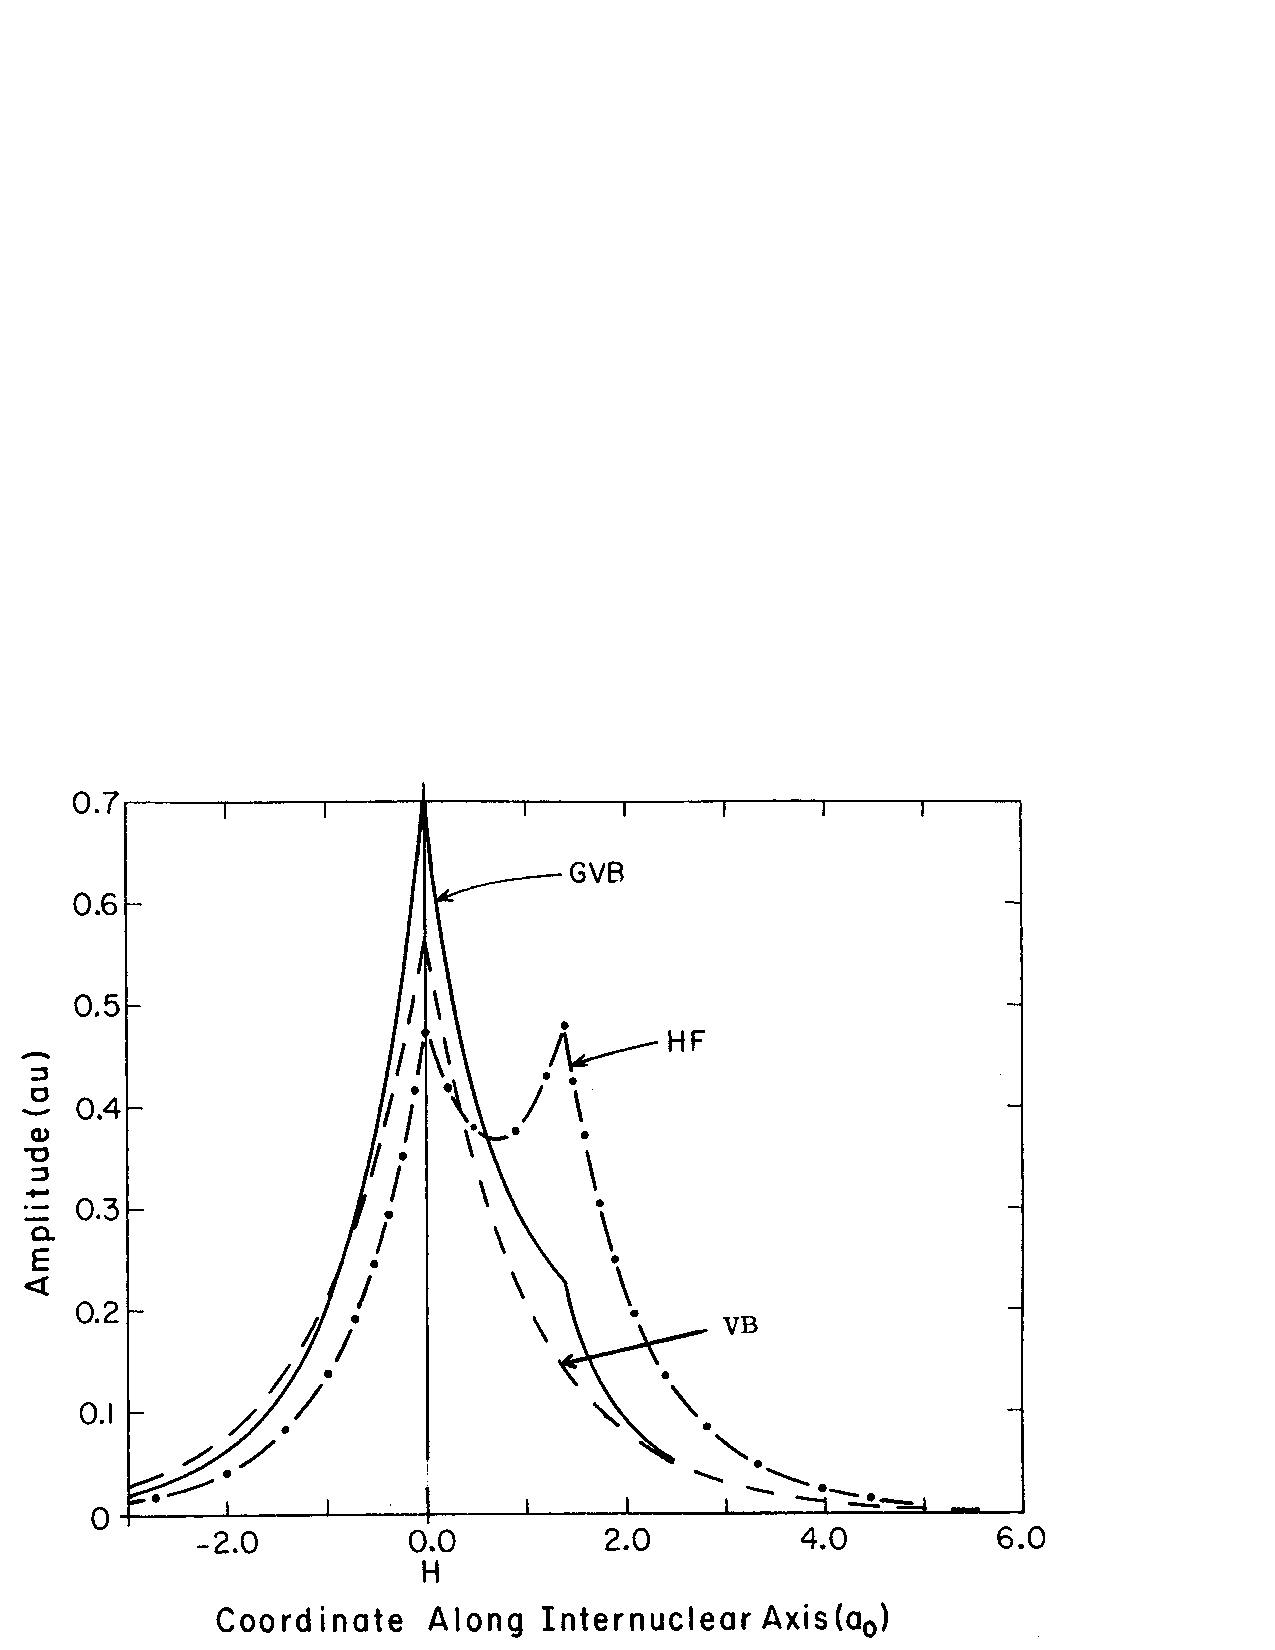
\includegraphics[scale=0.75]{fig3-08}
\caption{Comparsion of the GVB, VB and HF orbitals of H$_2$ at $R =
1.4a_0$.  Only one of the GVB and VB orbitals is shown.}
\label{fig3-09}
\end{figure}



\subsubsection{Interpretation}

If (\ref{chap3-eqno44}) is satisfied for all basis functions
$\chi_{\mu}$ of a complete set, then $\varphi_a$ satisfies the
differential equation
\begin{equation}
H^a \varphi_a = \epsilon_a \varphi_a .
\label{chap3-eqno47}
\end{equation}
The $H^a$ in (\ref{chap3-eqno47}), can be written as
\begin{equation}
H^a = h + V_b
\label{chap3-eqno48}
\end{equation}
where $V_b$ contains all the terms depending upon orbital $\varphi_b$.  We 
can consider $V_b$ as the average potential seen by the electron in 
$\varphi_a$ due to the electron in $\varphi_b$.  Note that $V_b$ is not a
local potential, that is, a function of ${\bf r}$.  Rather, $V_b$ 
contains integral operators and upon operating on $\varphi_a$ and $\varphi_b$ 
inside the integral.  Even so, we can consider $V_b$ as the effective
potential due to $\varphi_b$ as seen by $\varphi_a$.  The average potential 
is not just the Coulomb potential $J_b$ due to the electron on $\varphi_b$, 
as would be expected classically, but also contains other terms arising 
from the quantum mechanical form of the wavefunction.  However, these
additional terms are not chosen arbitrarily and indeed were determined 
through the variational principle, as the terms required, in order 
that $\varphi_a$ be the optimum orbital to place in the two-electron 
wavefunction.  Thus, we can consider the potential $V_b$ as the
quantum mechanical generalization of the classical Coulomb term for 
the interaction between electrons in overlapping orbitals $\varphi_a$ and 
$\varphi_b$.

The operator $H^a$, in (\ref{chap3-eqno48}) is equivalent to the
Hamiltonian for an electron moving in the potential due to the nuclei,
contained in $h$, plus a potential $V_b$ due to the electron in
orbital $\varphi_b$.  Since orbital $\varphi_a$ is an eigenfunction of
$H^a$ , we can interpret $\varphi_b$ as the eigenstate of an electron
moving in the average potential, $V_b$, due to the other electron of
the system.  Similarly, of course, we can interpret $\varphi_b$ as the
eigenstate of an electron moving in the average potential, $V_A$, due
to the other electron.  Thus, with this interpretation, we can
describe the two-electron system in terms of two one-electron systems,
each of which contains the average potential due to the other
electron.  Such a description of a multi-electron system, in terms of
electrons moving independently of each other, will be termed an
independent particle interpretation, IPI.  We will find, especially
for larger molecules, that such independent particle interpretations
will be very useful in understanding the wavefunctions.

It is important to note here that the independent particle
interpretation comes about from the one-particle Schr\"odinger
equation, such as (\ref{chap3-eqno47}), arising from application of the
variational principle to a special type of wavefunction
(\ref{chap3-eqno42}).  The real electrons of a molecule are quite
indistinguishable, and we do not imply that one of the electrons moves
in one orbital, say $\varphi_a$, while the other electron moves in the
other orbital, $\varphi_b$.  What we say is that the orbitals satisfy
a one-electron Schr\"odinger equation for which the field term is the
average potential of an electron in the other orbital.  This is not
the equation describing the moving of one of the real electrons.
However, consider the eigenstates of two fictitious, distinguishable
electrons, we do obtain the optimum orbitals for the many-electron
wavefunction (\ref{chap3-eqno42}).  It is really the orbitals which are
distinguishable here, not the electrons.

\subsubsection{GVB Natural Orbitals}

In order to obtain another view of the GVB wavefunction, 
we will define the GVB orbitals  $\varphi_g$ and 
$\varphi_u$ as the sum and difference of the GVB orbitals 
$\varphi_\ell$ and $\varphi_r$
\begin{equation}
\varphi_g = {(\varphi_\ell + \varphi_r ) \over D_g}
\label{chap3-eqno49a}
\end{equation}
\begin{equation}
\varphi_u = {(\varphi_r - \varphi_\ell ) \over D_u}
\label{chap3-eqno49b}
\end{equation}
where
\begin{equation}
D_g = \sqrt{2(1+S)}
\label{chap3-eqno50a}
\end{equation}
and
\begin{equation}
D_u = \sqrt{2(1-S)}
\label{chap3-eqno50b}
\end{equation}
and $S$  is the overlap of the GVB orbitals
\begin{equation}
S = \langle \varphi_\ell \vert \varphi_r \rangle .
\end{equation}
Rearranging (\ref{chap3-eqno49a})--(\ref{chap3-eqno49b}) leads to
\begin{equation}
2 \varphi_r = D_g \varphi_g + D_u \varphi_u
\end{equation}
and
\begin{equation}
2 \varphi_\ell = D_g \varphi_g - D_u \varphi_u
\end{equation}
and hence, the total wavefunction becomes
\begin{equation}
\Phi = \varphi_\ell \varphi_r + \varphi_r \varphi_\ell = {\left[ D^2_g \varphi_g \varphi_g - 
D^2_u \varphi_u \varphi_r \right] \over 2} ,
\end{equation}
Thus, we may view the GVB wavefunction in terms of $\varphi_\ell$ and
$\varphi_r$, where there is always one electron in $\varphi_\ell$ and
one in $\varphi_r$.  Or, one may view this wavefunction in terms of
GVB \emph{natural orbitals} $\varphi_g$ and $\varphi_u$, where part of
the time both electrons are in $\varphi_g$ and part of the time both
are in $\varphi_u$.  Here, $\varphi_g$ resembles the bonding orbital
and $\varphi_u$ the antibonding orbital.  The equivalence of these two
descriptions may be clear in Figure \ref{fig3-10}, where (d) and (g)
are equivalent.

\begin{figure}
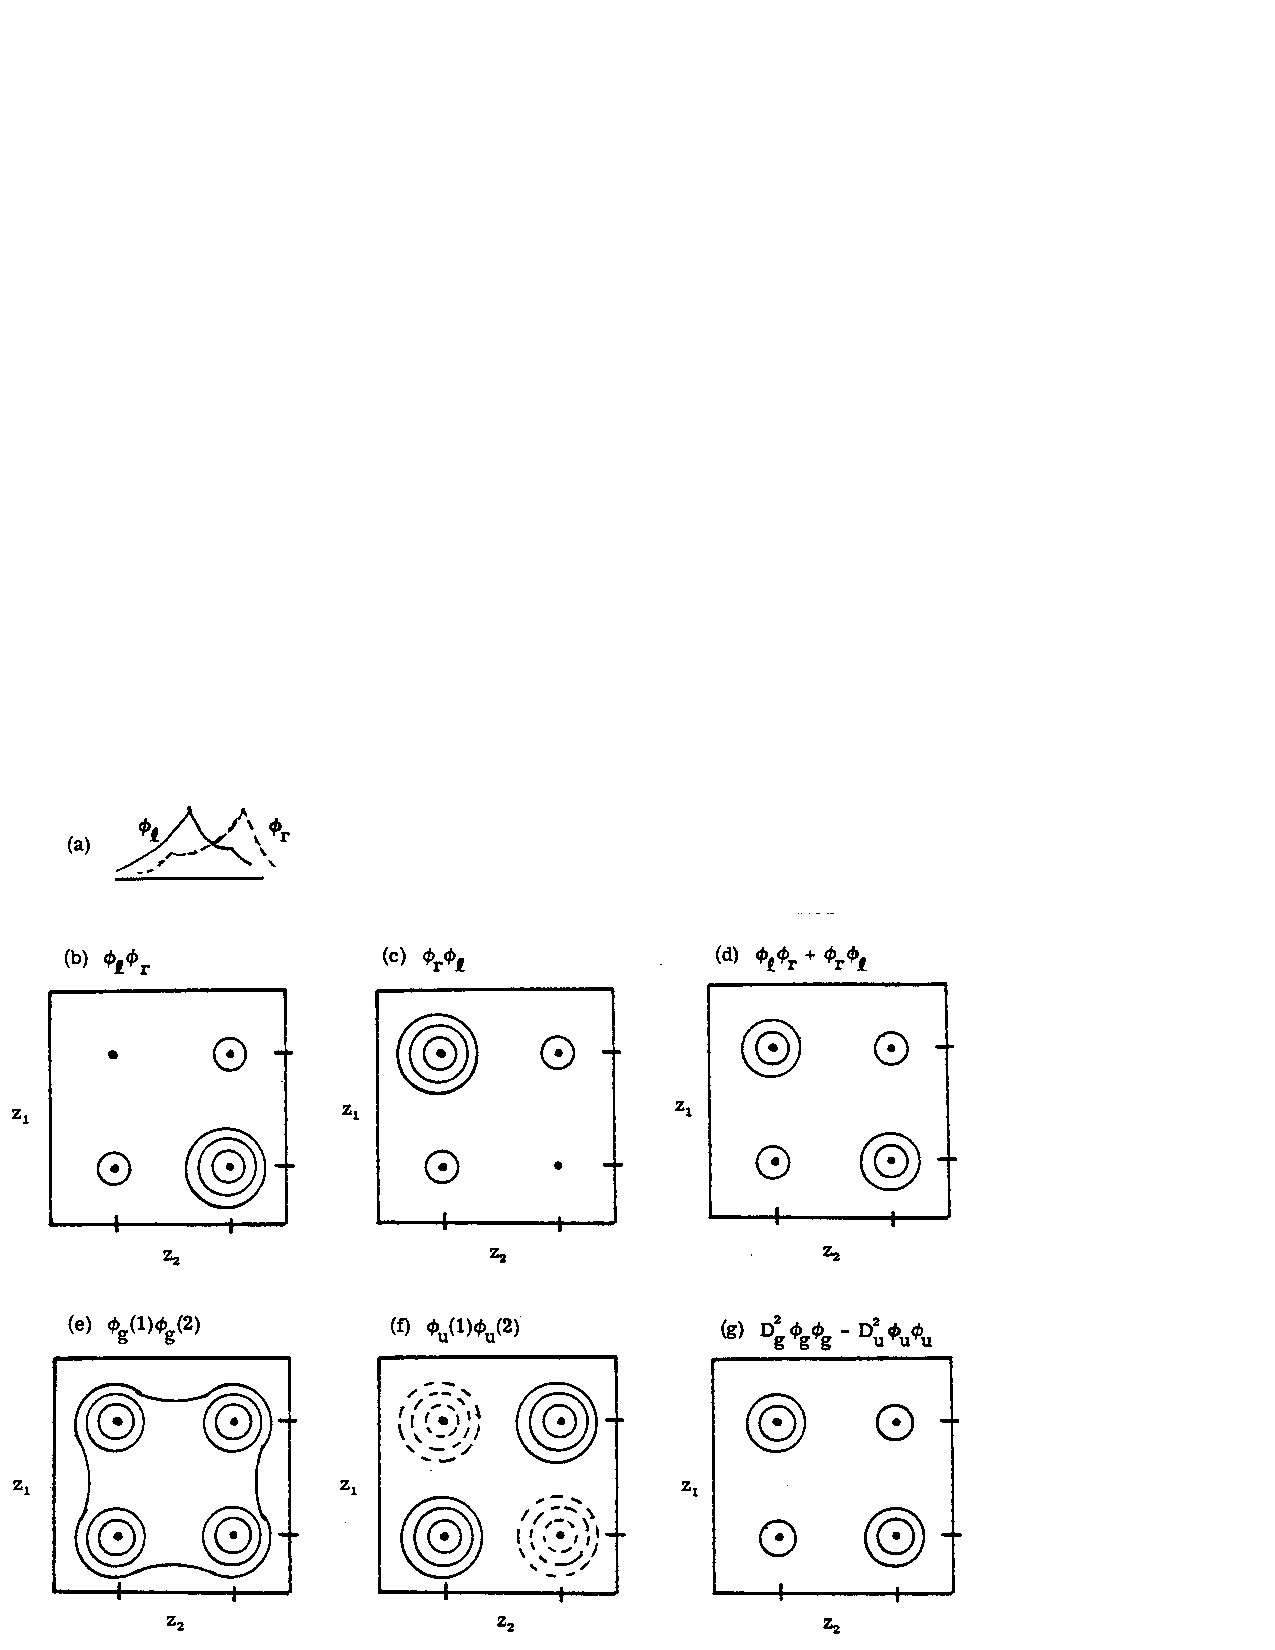
\includegraphics[scale=0.75]{fig3-09}
\caption{}
\label{fig3-10}
\end{figure}

The first natural orbital $\varphi_g$ has a good kinetic energy, but a bad 
two-electron energy.  Mixing in a small amount of $\varphi_u$ causes an 
increase in the kinetic energy, but this is more than compensated by the 
decrease in the electron repulsion energy, leading to the optimum 
wave function in Figure \ref{fig3-10} (d) or (g).

Requiring that the total wavefunction be normalized, leads to
\begin{equation}
\Phi = {( \varphi_\ell \varphi_r + \varphi_r \varphi_\ell ) \over
\sqrt{2(1+S^2)}} = C_g \varphi_g \varphi_g - C_u \varphi_u \varphi_u
\end{equation}
where from (\ref{chap3-eqno50a})--(\ref{chap3-eqno50b}),
\begin{equation}
{C_u \over C_g} = {D^2_u \over D^2_g} = {(1-S) \over (1+S)}
\end{equation}
That is, if the overlap between the two orbitals is nearly zero, H$_2$ 
for $R \rightarrow \infty$, then the two configurations come in with nearly 
equal coefficients.  On the other hand, for H$_2$ at $R = 1\ a_0$, and 
$S = 0.8$, and hence
\begin{equation}
{C_u \over C_g} = {1 \over 9} = 0.11.
\end{equation}

In this section, we use $g$ and $u$ for the orbitals as appropriate for 
H$_2$.  However, the discussion does not depend upon inversion symmetry 
and all results apply also to the GVB pair for an 
unsymmetric system.

\subsection{Electron Correlation}

In a real atom, the electrons are expected to move somewhat in concert so 
that they avoid getting too close to each other while remaining close to 
the nucleus.  That is, their motions are somewhat correlated.  On the other 
hand, in the HF wavefunction, $\varphi(1) \varphi(2)$, each electron is 
placed in the same orbital and, hence, the probability of either
electron being at a particular position, is independent of where the other 
electron is.  That is, the electrons in the HF orbital are 
uncorrelated in their motions.  For this reason, the different between the 
HF energy and the exact energy is called the
correlation error.  For the ground state of two-electron atoms, H$^-$, 
He, Li$^+$, etc., the correlation error is about 1.1 eV.  In addition, for 
H$_2$, at $R_e$, the correlation error is 1.1 eV.  Although this correlation 
energy is small compared to the total energy of these system, e.g., 1.5\% 
of He, it is comparable to many quantities of interest.

In the GVB wavefunction of H$_2$
\begin{equation}
\varphi_\ell ( 1 ) \varphi_r ( 2) + \varphi_r ( 1 ) \varphi_\ell ( 2 ) ,
\label{chap3-eqno51}
\end{equation}
one electron is in $\varphi_\ell$, while the other electron is in $\varphi_r$, 
regardless of which electron is in which.  Hence, there is static correlation 
in the sense that the orbitals for each electron are in a slightly 
different region of space, and hence, on the average, the electrons stay 
farther apart.  However, the presence of electron 1 at a
particular location of the $\varphi_\ell$ orbital, does not affect the probability 
of electron 2 being at any particular position in orbital $\varphi_r$, and 
hence, we may consider that the GVB wavefunction does 
not provide for instantaneous correlations among the motions of the 
electrons.  Since the GVB wavefunction is the most
general wavefunction involving just two spatial orbitals, we may consider 
that all correlation error beyond GVB involves 
instantaneous correlation of the electrons.  When important to distinguish 
these effects, we will refer to the latter as dynamic electron correlations 
and the difference between HF and GVB as 
static electron correlation.

Now consider the description of correlation in the natural orbital (NO)
representation of the GVB wavefunction
\begin{equation}
\Phi^{NO}_{(1,2)} = C_g \varphi_g(1) \varphi_g (2) - C_u 
\varphi_u(1)\varphi_u(2).
\label{chap3-eqno52}
\end{equation}
Assume that electron 1 is at some position $R$ on the right side of the 
molecule, and consider the likelihood of electron 2 being at equivalent 
positions $R$ or $L$ on the right and left sides of the molecule. In the 
HF wavefunction
\begin{equation}
\Phi^{HF} (R,R) = \varphi(R) \varphi(R)
\end{equation}
\begin{equation}
\Phi^{HF} (R , L) = \varphi (R) \varphi(L) ,
\end{equation}
and since $\varphi(R) = \varphi(L)$, we have equal probabilities
\begin{equation}
\vert \Phi^{HF} (R , R) \vert^2 = \vert \Phi^{HF} (R , L) \vert^2
\end{equation}
of the electrons being on the same, or opposite, sides.  In the GVB
wavefunction (\ref{chap3-eqno51}), we find 
\begin{equation}
\Phi^{GVB} (R , R) = \varphi_\ell ( R ) \varphi_r (R) + \varphi_r (R) \varphi_\ell(R)
\end{equation}
and
\begin{equation}
\Phi^{GVB} (R , L) = \varphi_\ell ( R ) \varphi_r (L) + \varphi_r (R) \varphi_\ell(L) ,
\end{equation}
and hence,
\begin{equation}
\Phi^{GVB} (R,R) < \Phi^{GVB} (R,L),
\label{chap3-eqno53}
\end{equation}
that is, we obtain the static correlation referred to above.  Using the 
NO form of the wavefunction, we obtain

\begin{eqnarray}
\Phi^{NO} (R,R) &= C_g \varphi_g (R) \varphi_g(R) - C_u \varphi_u (R) \varphi_u 
(R)\\
\Phi^{NO} (R,L) &= C_g \varphi_g (R) \varphi_g (L) - C_u \varphi_u (R) \varphi_u 
(L)\\
&= C_g \varphi_g (R) \varphi_g (R) + C_u \varphi_u (R) \varphi_u (R)\cr
\end{eqnarray}

\noindent using the symmetries of $\varphi_g$ and $\varphi_u$, and hence,
\begin{equation}
\Phi^{NO} (R,R) < \Phi^{NO}(R,L)
\end{equation}
just as in (\ref{chap3-eqno53}).  Comparing (\ref{chap3-eqno52}) with
the HF wavefunction
\begin{equation}
\Phi^{HF} (1,2) = \varphi_g (1) \varphi_g (2)
\end{equation}
we see that in order to obtain effective electron corrilation, the
second natural orbital must have a shape similar to that of the first,
dominant, natural orbital, but with an extra nodal plane bisecting the
first natural orbital.  This allows maximal difference between
$\Phi^{NO} (R, R)$ and $\Phi^{N0} (R , L)$, and hence, maximal
electron correlation. We will, later, find such arguments in terms of
nodal planes to be useful in describing other electron correlation
effects. This discussion should all be clear from Figure
\ref{fig3-10}.

\subsubsection{Ionization Potentials}

In general, we expect the correlation error to increase with the number 
of electrons, since there are more and more complicated interrelationships 
ignored.  Thus, the ionization potentials calculated from the HF 
and GVB should be too small.  On the other hand, we 
can get an approximate independent particle from Koopmans' theorem.  The 
Koopmans independent particle is the energy difference between the 
self-consistent energy of the $N$-electron system, $E_N$, and an energy 
of the $N-1$ electron system, $E_{N-1}$, obtained using orbitals from 
the $N$-electron wavefunction.  Thus, the description of the ionic, $N - 1$ 
electron, state is nonoptimum leading to too high a value for $E_{N-1}$ 
and, hence too large a prediction of independent particle.  However, the
independent particle calculated using self-consistent wavefunctions of 
the $N$ and $N - 1$ electron systems, should be too small.  Hence, there 
is a cancelling of errors such that the Koopmans theorem value of 
independent particle is usually rather good, within about
10\%. These effects are indicated in Figure \ref{fig3-11}.


\begin{figure}
\begin{center}
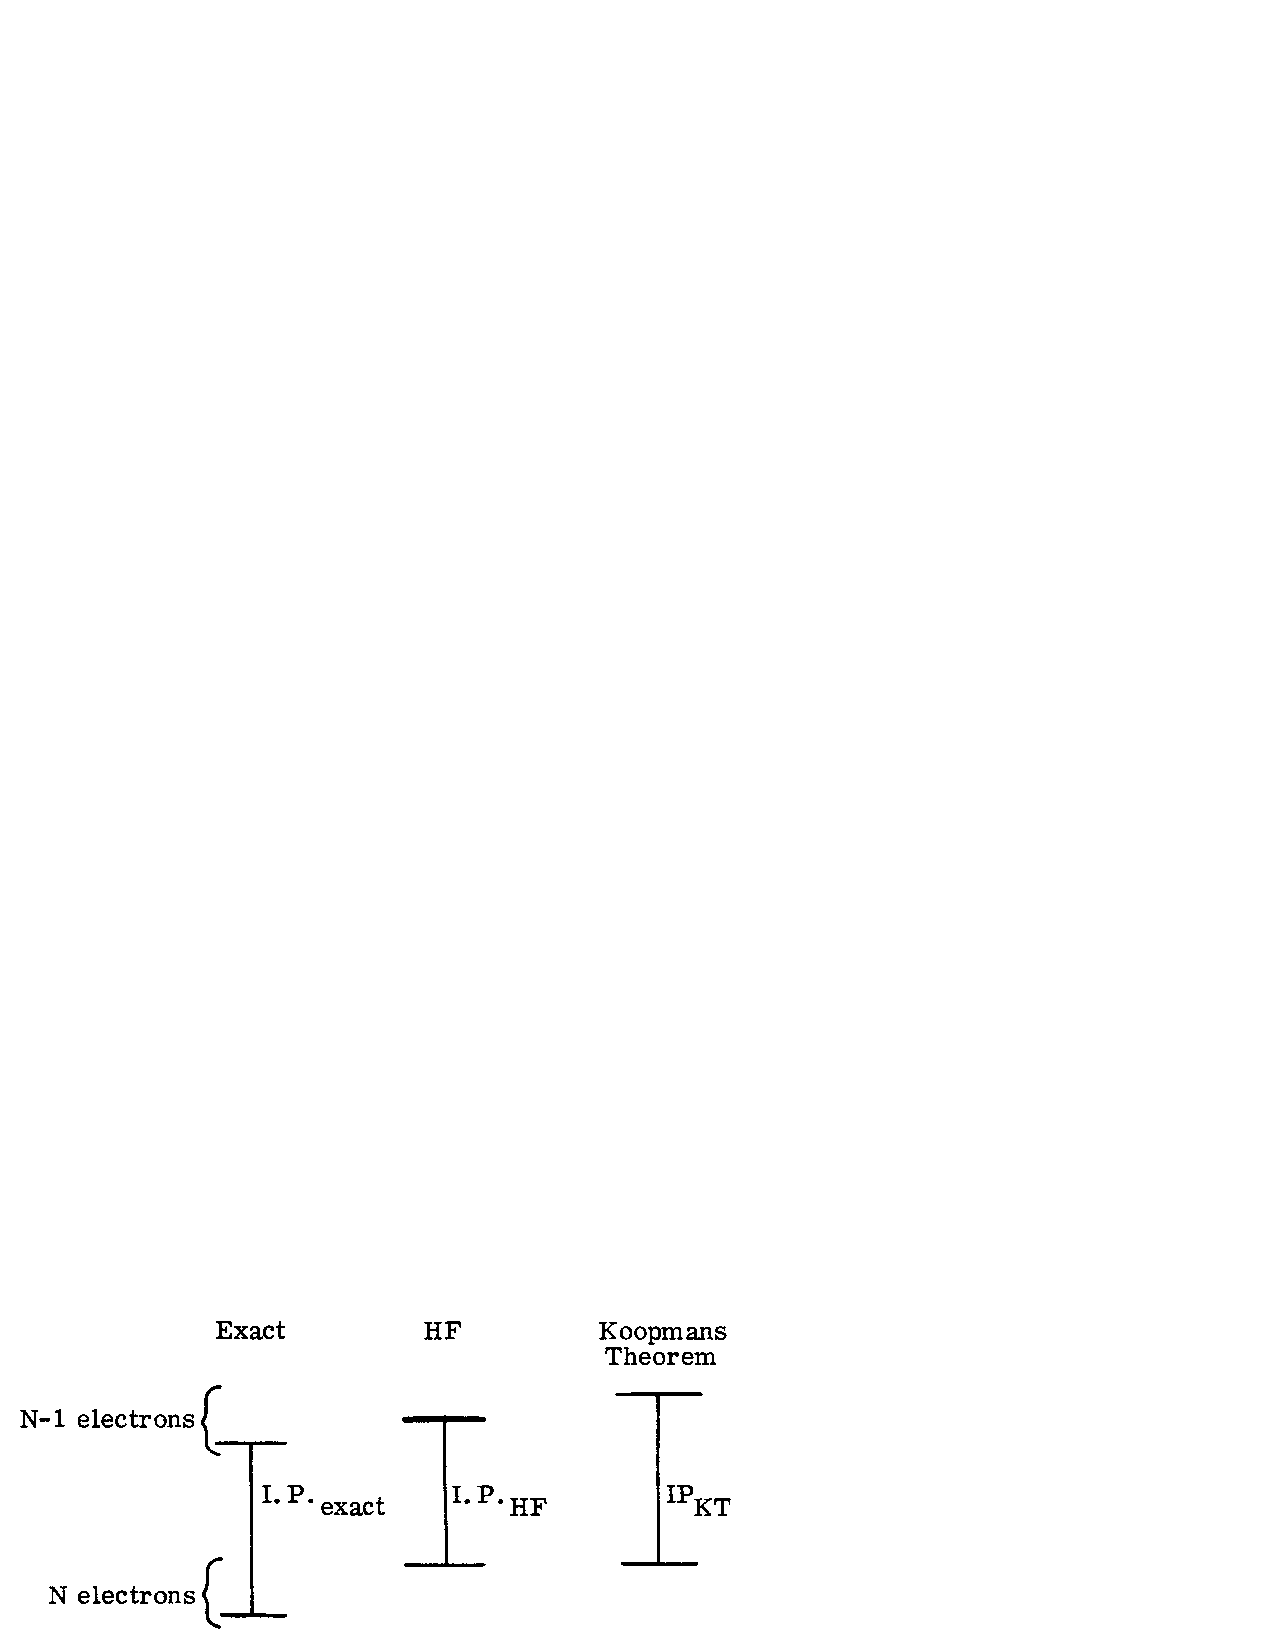
\includegraphics[scale=0.75]{fig3-10}
\end{center}
\caption{}
\label{fig3-11}
\end{figure}

\subsection{CI Wavefunctions}

Starting with a one-electron basis
\begin{equation}
\left\{ \chi_{\mu} : \mu = 1 , 2 , \cdot \cdot \cdot  P \right\}
\end{equation}
we can construct a two-electron basis
\begin{equation}
\left\{ \chi_{\mu} (1) \chi_{\nu} (2) ; \mu , \nu = 1 , 2 , \cdot 
\cdot \cdot P \right\}
\end{equation}
by combining all products of one-electron functions. In terms of this 
basis, the most general wavefunction is
\begin{equation}
\Phi (1,2) = \sum^P_{\mu , \nu = 1} C_{\mu \nu} \chi_{\mu} (1) 
\chi_{\nu} (2) .
\label{chap3-eqno54}
\end{equation}
The terms in (\ref{chap3-eqno54}) are called \emph{configurations},
and the resulting wavefunction is called a \emph{CI wavefunction}.


Applying the variational principle from earlier, the optimum
coefficients for (\ref{chap3-eqno54}) are solutions of the equation
\begin{equation}
\sum_{\mu\nu}(H_{\mu\nu,\sigma\eta}-E)C_{\mu\nu} = 0.
\end{equation}
For a complete basis ($P \rightarrow \infty$) the resulting CI
wavefunction is the exact wavefunction of the system.

\subsubsection{Permutational Symmetry}

Because the electrons are identical, the Hamiltonian must be invariant
(unchanged) upon permutation (interchange) of the electrons
\begin{equation}
H ( 2 , 1 ) = H ( 1 , 2 ).
\label{chap3-eqno55}
\end{equation}
As a result of this permutational symmetry, the exact eigenstates 
of $H$ can always be taken as either symmetric
\begin{equation}
\Psi^s (2,1) = \Psi^s (1,2)
\label{chap3-eqno56}
\end{equation}
or antisymmetric
\begin{equation}
\Psi^a (2,1) = - \Psi^a (1,2)
\end{equation}
under permutation. The proof is quite analogous to that in Chapter 2
where we found that for a system with inversion symmetry, all
eigenfunctions are either $g$ or $u$.

Later, when we discuss the Pauli principle and spin, we will find that
symmetric spatial wavefunctions $\Psi^s$ are allowed only for singlet
($S = 0$) spin states and antisymmetric spatial wavefunctions $\Psi^a$
are allowed only for triplet ($S = 1$) spin states.

\subsubsection{The Nodal Theorem}

Next we will show that the lowest state of $H(1,2)$ (assuming $H$ is
symmetric (\ref{chap3-eqno55})) is always a symmetric wavefunction,
$\Psi^s (1 , 2)$, (\ref{chap3-eqno56}).

\begin{figure}
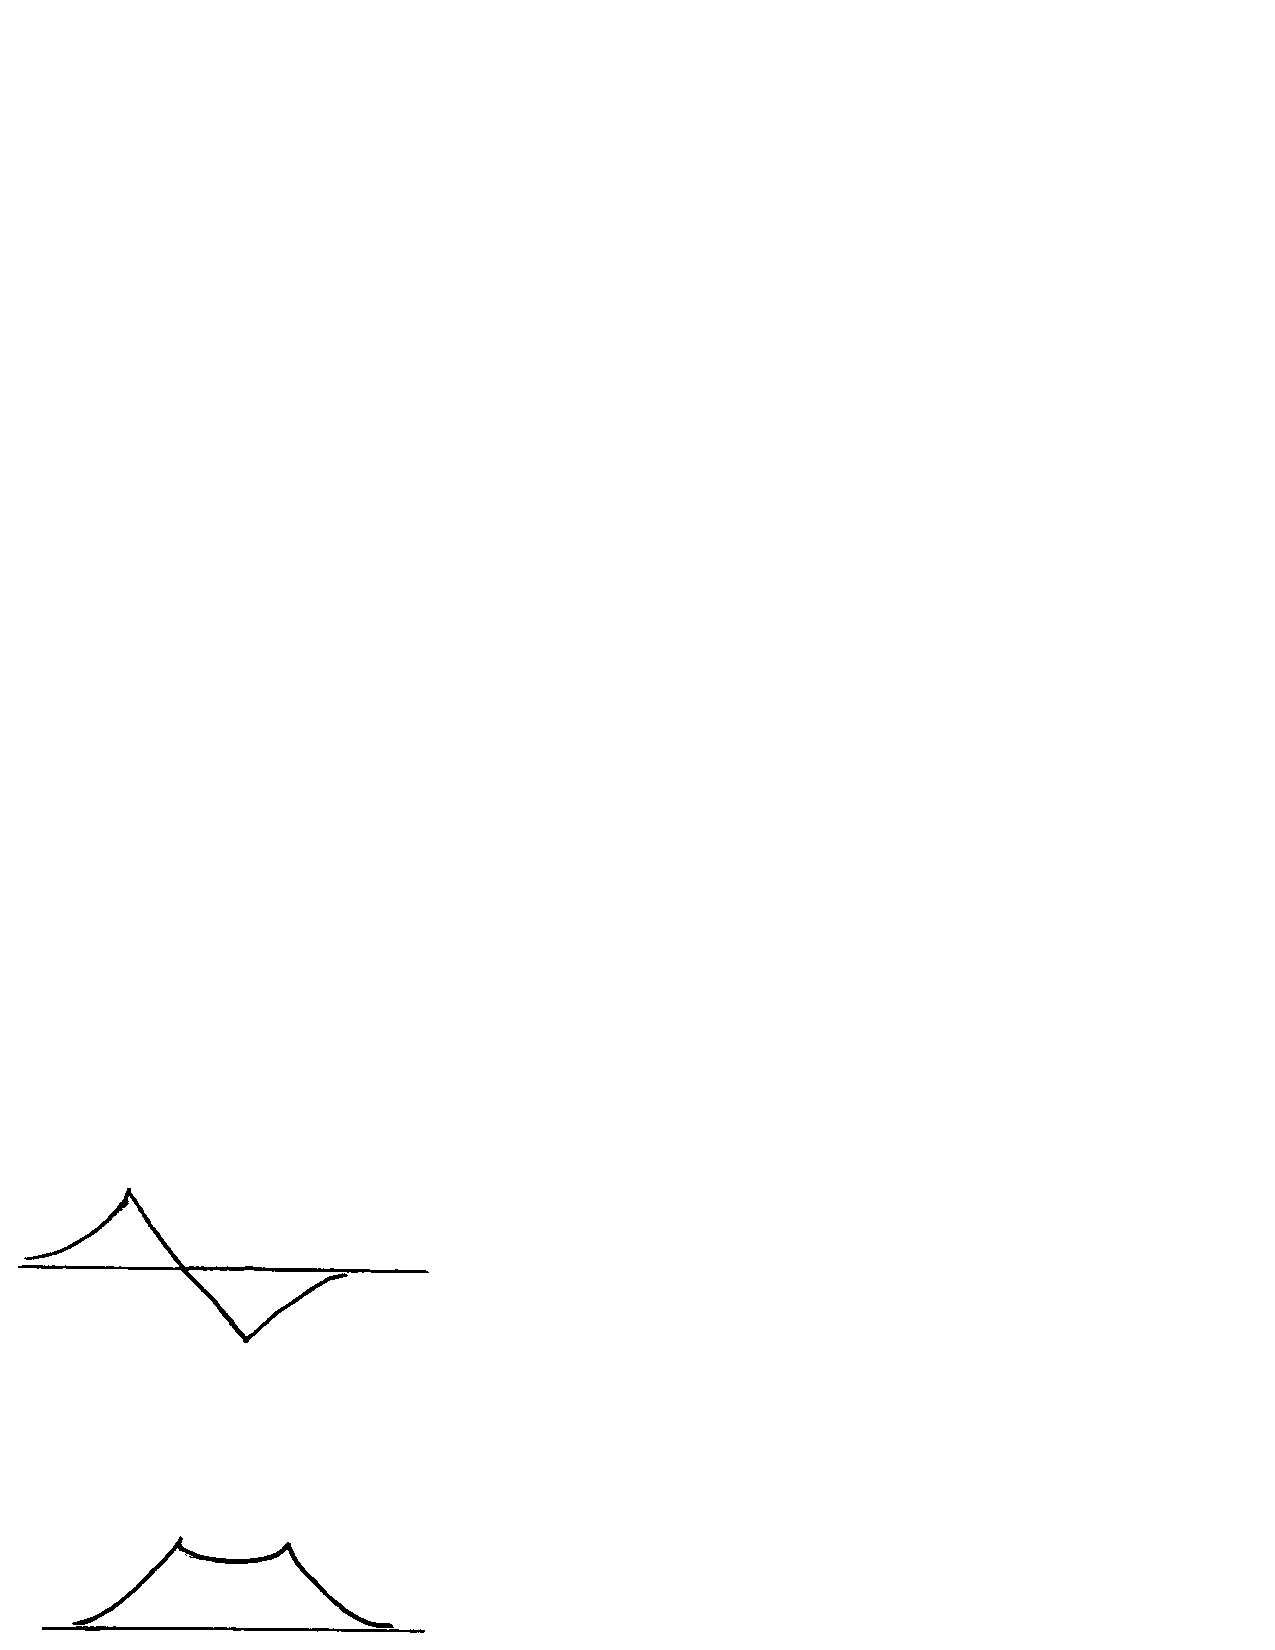
\includegraphics[scale=0.75]{fig3-10-1}
\caption{LCAO combinations with (top) and without (bottom) a node.}
\label{fig3-10-1}
\end{figure}

As shown in Chapter 1, the ground state of a system is nodeless, that is, 
the wavefunction of the ground state has the same sign everywhere. For a 
one-electron system, this means that the top wave function in Figure
\ref{fig3-10-1} cannot be the ground state, except for $R = \infty$,
where this state is degenerate with the nodeless state.  Whereas
the bottom state in Figure \ref{fig3-10-1} can.  The nodal theorem
applies also for many electron systems, such as 
\begin{equation}
H (1,2) = - {1 \over 2} \nabla^2_1 - {1 \over 2} \nabla^2_2 + 
v(r_1) + v(r_2) + {1 \over r_{12}}
\label{chap3-eqno57}
\end{equation}
(the proof is exactly as in Chapter 1). We will now use the nodal
theorem to show that the ground state of any two-electron system must
be a symmetric wavefunction.

Letting ${\bf r}_1 = {\bf r}_2$ in a antisymmetric wavefunction
\begin{equation}
\psi^a \left( {\bf r}_2 , {\bf r}_1 \right) = - \psi^a \left( {\bf 
r}_1 , {\bf r}_2 \right)
\end{equation}
leads to
\begin{equation}
\psi^a \left( {\bf r}_1 , {\bf r}_1 \right) = - \psi^a \left( {\bf
r}_1 , {\bf r}_1 \right)
\end{equation}
and hence,
\begin{equation}
\psi^a \left( {\bf r}_1 , {\bf r}_2 \right) =0
\end{equation}
if ${\bf r}_1 = {\bf r}_2$.  (For example, typical one-dimensional cases 
are illustrated in  Figure \ref{fig3-12}.)

\begin{figure}
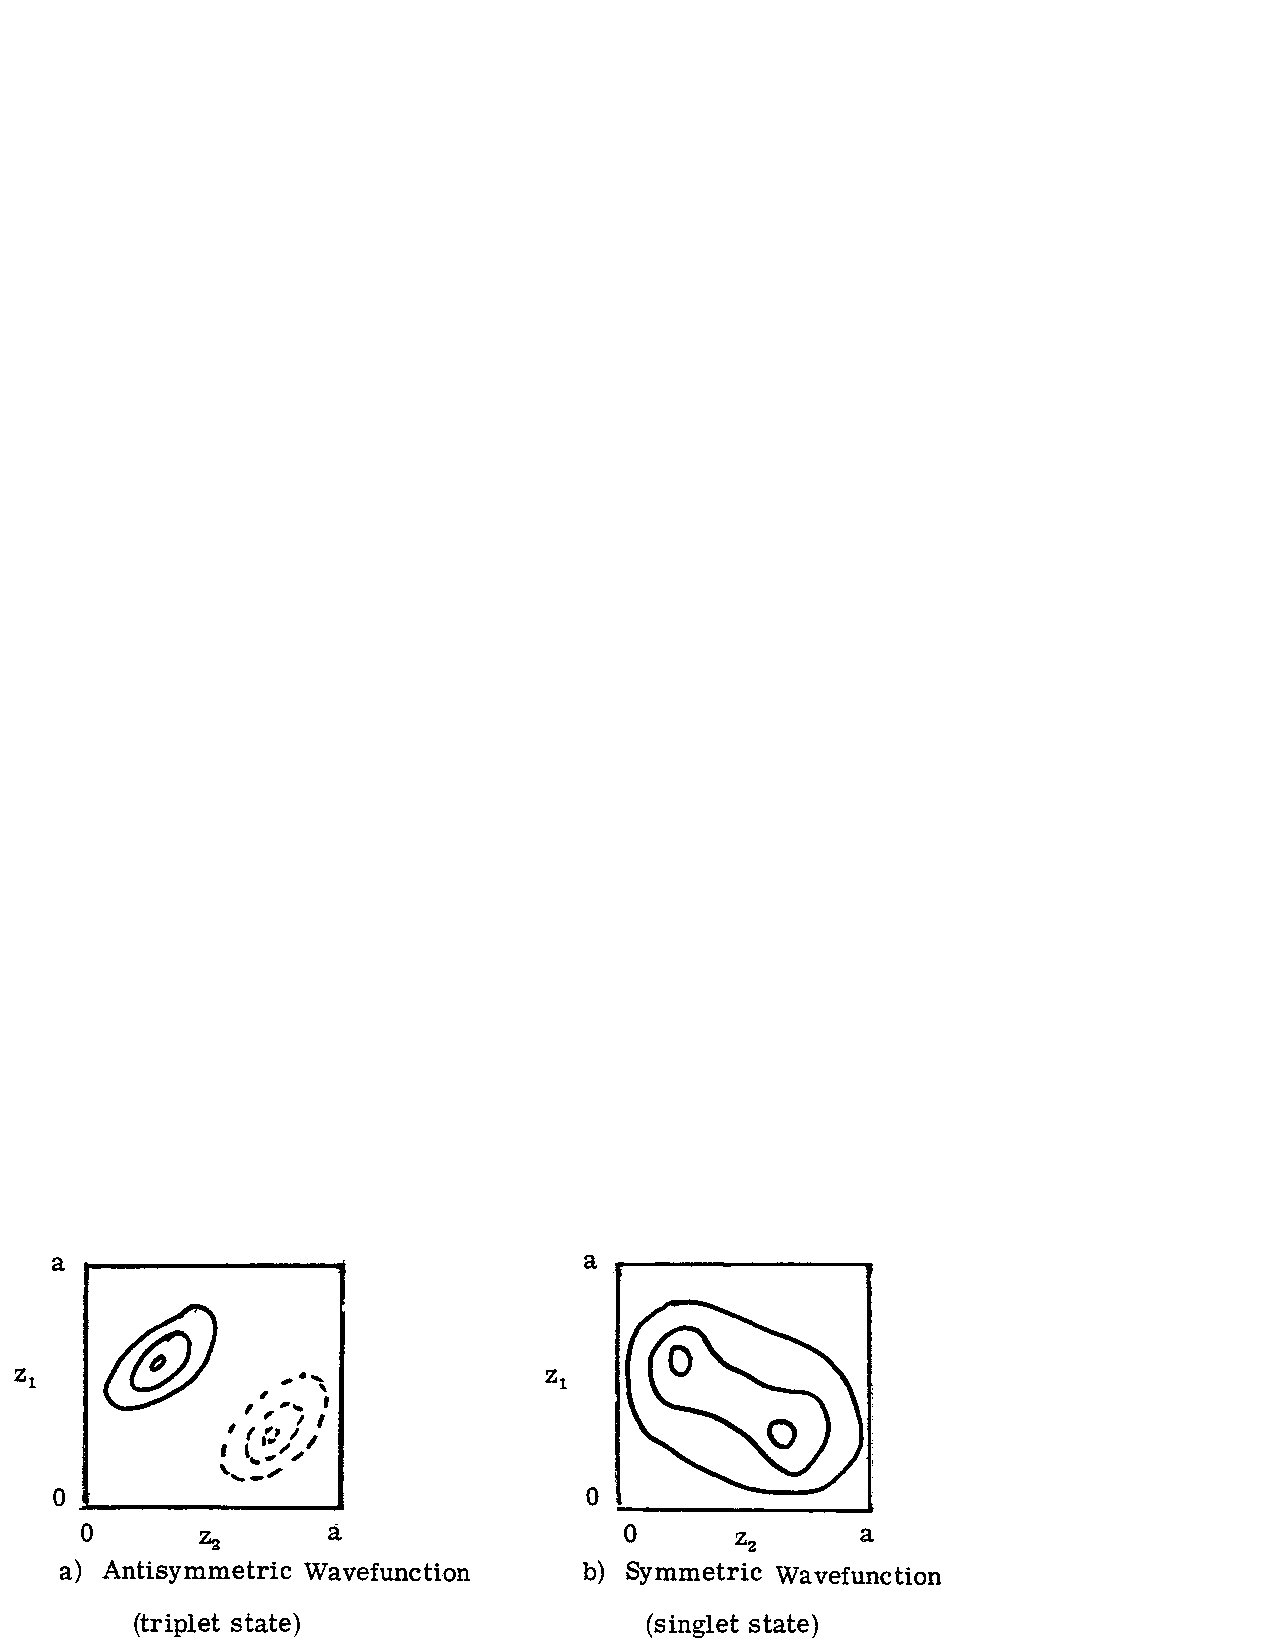
\includegraphics[scale=0.75]{fig3-11}
\caption{Illustration of nodal patterns of two-electron systems, in
one dimension.}
\label{fig3-12}
\end{figure}

Thus, every antisymmetric function has a nodal plane, whereas,
symmetric functions need not have nodal planes. Since the nodal
theorem implies that the ground state is nodeless, then the ground
state must be permutationably symmetric (\ref{chap3-eqno56}).  Later,
we will find that a symmetric spatial wavefunction must correspond to
a singlet spin state and, hence, the ground state of a two-electron
system must be a singlet state.

In the case of a sufficiently singular potential, it is possible for
the lowest wavefunction having a node to be as low as the lowest
nodeless wavefunction.  However, in three dimensions, our Hamiltonian
(\ref{chap3-eqno57}) is not this singular and, hence, the inequalities
apply.

\subsubsection{Natural Orbitals}

In Section \ref{chap3-app-b} we show that the CI wavefunction
(\ref{chap3-eqno54}) for the ground state of any two-electron system,
can be written as
\begin{equation}
\Psi^0 (1,2) = \sum_{\mu =1} {\bar C}_{\mu} {\bar \chi}_{\mu} (1) 
{\bar \chi}_{\mu} (2)
\label{chap3-eqno58}
\end{equation}
(that is, double occupied orbitals only) where the orbitals $\{ {\bar
\chi}_{\mu} \}$, called \emph{natural orbitals}, are orthonormal
\begin{equation}
\langle {\bar \chi}_{\mu} \vert {\bar \chi}_{\nu} \rangle 
=\delta_{\mu \nu} .
\end{equation}
Since (\ref{chap3-eqno58}) has only $P$ terms rather than $P^2$, as in
(\ref{chap3-eqno54}), it is obviously easier to interpret.

The density of electrons in a two-electron system is defined as
\begin{equation}
\rho(1) = \int d^3 r_2 \Psi(1,2)^* \Psi(1,2) .
\end{equation}
Thus, using (\ref{chap3-eqno58}) leads to
\begin{equation}
\rho(1) = \sum_{\mu , \nu} {\bar C}^*_{\mu} {\bar C}_{\nu} {\bar 
\chi}_{\mu} (1)^* {\bar \chi}_{\nu}(1) \langle \chi_{\mu}(2) \vert 
\chi_{\nu} (2) \rangle = \sum_{\mu} p_{\mu} \vert \chi_{\mu} (1) \vert^2
\end{equation}
where
\begin{equation}
p_{\mu} = \vert C_{\mu} \vert^2 .
\end{equation}
Since there is a total of two electrons in the system
\begin{equation}
\int d^3 r_1 \rho(1) = 2 ,
\end{equation}
the coefficients must sum to two,
\begin{equation}
\sum_{\mu} p_{\mu} = 2 .
\end{equation}
Consequently, in terms of natural orbitals, the total density of the
CI wavefunction is just the sum of the densities of the natural
orbitals weighted by a population $p_{\mu}$ that sums to two.

\section{Wavefunctions of He}

In this section, we will illustrate the HF, GVB, and CI methods by
describing the wavefunctions for He atom.

\subsection{HF Wavefunctions for the He Atom}

First, we consider various approximations of the HF
wavefunction
\begin{equation}
\Phi^{HF} (1,2) = \varphi(1) \varphi(2) ,
\end{equation}
where the HF orbital $\varphi$ is expanded in a basis set.

\subsubsection{MBS}

The simplest description of He atom is to place two electrons in the 
$1s$ orbital of He$^+$
\begin{equation}
\chi = e^{- \zeta r}
\end{equation}
where $\zeta = 2.0$.  The total energy in hartrees is just
\begin{equation}
E = 2 \epsilon_1 + J = - 2.75 ,
\end{equation}
where $\epsilon_1 = -2.0$ is the energy of He$^+$, and
\begin{equation}
J = {5 \over 8} \zeta = 1.25 ,
\end{equation}
is the Coulomb interaction of the two electrons, see Section
\ref{chap3-app-c}.

This description can be improved by optimizing $\zeta$, leading to the
MBS description.  As shown in Section \ref{chap3-app-c}, the energy
has the form
\begin{equation}
E = \zeta^2 T_1 + \zeta V_1 ,
\end{equation}
where
\begin{equation}
T_1 = (2) \left( {1 \over 2} \right) = 1
\end{equation}
and
\begin{equation}
V_1 = - 2 Z + {5 \over 8}
\end{equation}
(i.e., $T_1$ and $V_1$ are the kinetic and potential energies for the
case of $\zeta = 1$).  Requiring that
\begin{equation}
{\partial E \over \partial \zeta} = 0 ,
\end{equation}
to obtain the optimum $\zeta$, leads to
\begin{equation}
\zeta_{OPT} = - {V_1 \over 2T_1} = Z - {5 \over 16} = 1.6875
\label{chap3-eqno60}
\end{equation}
for He. Since the optimum $\zeta$ for the one-electron atom is $\zeta
= Z$, we can interpret the $\zeta_{OPT}$ as an effective charge that
has decreased from $Z$ due to the presence of the second electron.  It
is as if the second electron partially shields the nucleus.  Hence,
the quantity
\begin{equation}
\sigma = {5 \over 16}
\end{equation}
is sometimes referred to as the \emph{shielding correction}.

Substituting (\ref{chap3-eqno60}) into
(\ref{chap3-eqno59a})--(\ref{chap3-eqno59b}) leads to
\begin{equation}
E_{OPT}  - {V^2_1 \over 4T_1} = + {V_1 \over 2} \zeta_{OPT} = - 
\zeta^2_{OPT}  = -2.84766h.
\label{chap3-eqno61}
\end{equation}
This energy is the same as if there had been two non-interacting electrons, 
each experiencing the Coulomb field due to a nucleus of charge
\begin{equation}
\zeta_{OPT} = Z - {5 \over 16} .
\end{equation}

The exact energy for He atom is $-2.9037$.  Thus, the above simple
wavefunction accounts for 98.5\% of the exact energy. Since the
correct energy of He$^+$ is $-2.0$, the use of the calculated $E$ of
(\ref{chap3-eqno61}), leads to a predicted independent particle of
0.84766 or 94\% of the exact value. Use of the Koopmans theorem leads
to
\begin{equation}
- IP = \langle \varphi \vert h \vert \varphi \rangle + J_{\varphi \varphi} = {1 
\over 2} \zeta^2_{OPT} = Z \zeta_{OPT} + {5 \over 8} \zeta_{OPT} = - 
{1 \over 2} \zeta^2_{OPT} + {5 \over 16} \zeta_{OPT} = - 0.89648 ,
\end{equation}
99.2\% of the experimental value (a better value is obtained because
we describe the ion badly).

\subsubsection{Bigger Basis Sets}

\begin{table}
\caption{Parameters of HF wavefunctions of the 
ground state of He. $E$ is the total energy, $E$ is the orbital
energy. The orbital exponents are shown in parentheses, while the
expansion coefficients are not. All quantities are in Hartree atomic
units.}

\begin{tabular}{ccccc} \\ \hline
P & 1 & 2$^a$ & 3$^a$ & 12$^b$\\
$E$ &$-$2.847656 & $-$2.861673 & $-$2.861680 & $-$2.861680\\
$\epsilon$ & $-$0.89648 & $-$0.91792 & $-$0.91795 & $-$0.91796\\ \hline
ns$(\zeta)C_i$&$1s$(l.68750)1.0&$1s$(l.453)0.84289&$1s$(l.450)1.36211
&$1s$(3.0) 0.45742\\
&&$1s$(2.906)0.18159&$2s$(l.723)-0.28189&$1s$(1.4) 0.00000\\
&&&$2s$(2.641)-0.10724&$2s$(3.0) 0.24427\\
&&&&$2s$(1.4) 0.12985\\
&&&&$3s$(3.0) 0.13657\\
&&&&$3s$(1.4) 0.11340\\
&&&&$4s$(3.0) 0.09451\\
&&&&$4s$(1.4)$-$0.08606\\
&&&&$5s$(3.0) 0.00819\\
&&&&$5s$(1.4) 0.02546\\
&&&&$6s$(3.0) 0.02767\\
&&&&$6s$(1.4)$-$0.00267\\ \hline 
\end{tabular}\\
$^a$See reference 19.  $^b$See reference 20.
\end{table}

\begin{figure}
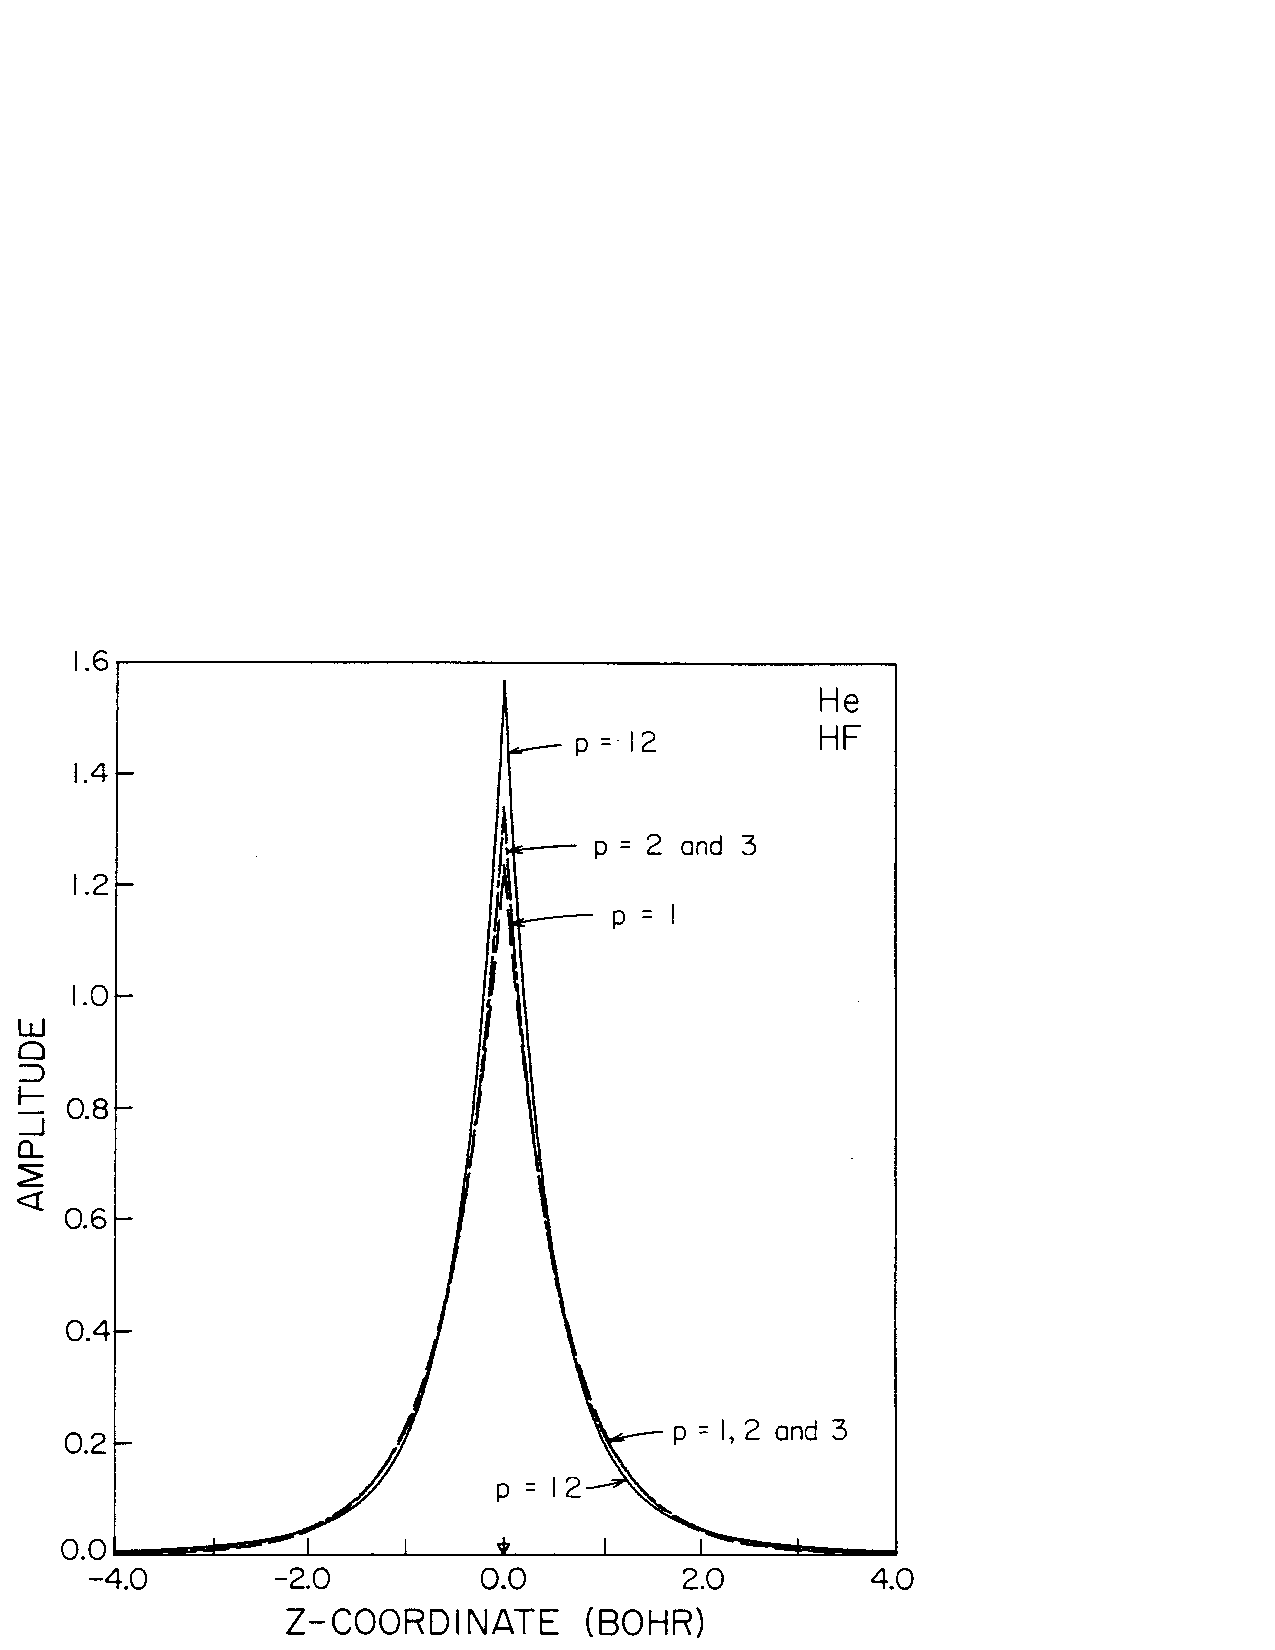
\includegraphics[scale=0.75]{fig3-12}
\caption{Comparison of HF wavefunctions for He using various (optimum)
basis sets.  $p$ indicates the number of functions in the basis set.}
\label{fig3-13}
\end{figure}

The results of using various-sized basis sets for HF calculations on
He, are listed in Table \ref{table3-02}. In the cases $P = 1, 2$, and
3, extensive optimization of the parameters was carried out, leading
to quite short expansions. Thus, with $P = 2$ we are within 0.000007 h
= 0.0002 eV = 0.005 kcal/mol of the HF limit ($P = \infty$). With $P =
3$, the energy is correct to 6 decimal places, comparing to the HF
limit.  Bear in mind here that the exact, nonrelativistic, energy for
He is $-$2.903 so that even the exact HF wavefunction is off by 0.042
h = 1.1 eV = 25 kcal/mol. The HF orbitals in these various
approximations, are plotted in Figure \ref{fig3-13}. Note that even
though $P = 3$ and $P = 12$ lead to the same energy, to 6 decimal
places, there are still noticeable change in the orbitals. The
conclusion is that two suitably chosen basis functions are adequate
for describing He. Such a basis is referred to as \emph{double zeta}
(DZ) or \emph{double valence} (DV).

\subsection{The GVB Wavefunctions for the He Atom}

For He atom, the GVB wavefunction is the optimum
wavefunction of the form
\begin{equation}
\Phi^{GVB} (1,2) = \varphi_a (1) \varphi_b (2) + \varphi_b (1) \varphi_a (2)
\end{equation}
The GVB orbitals of He are shown in Figure
\ref{fig3-14}, where they are compared to the $1s$ orbital of He$^+$
and to the HF orbital of He.

\begin{figure}
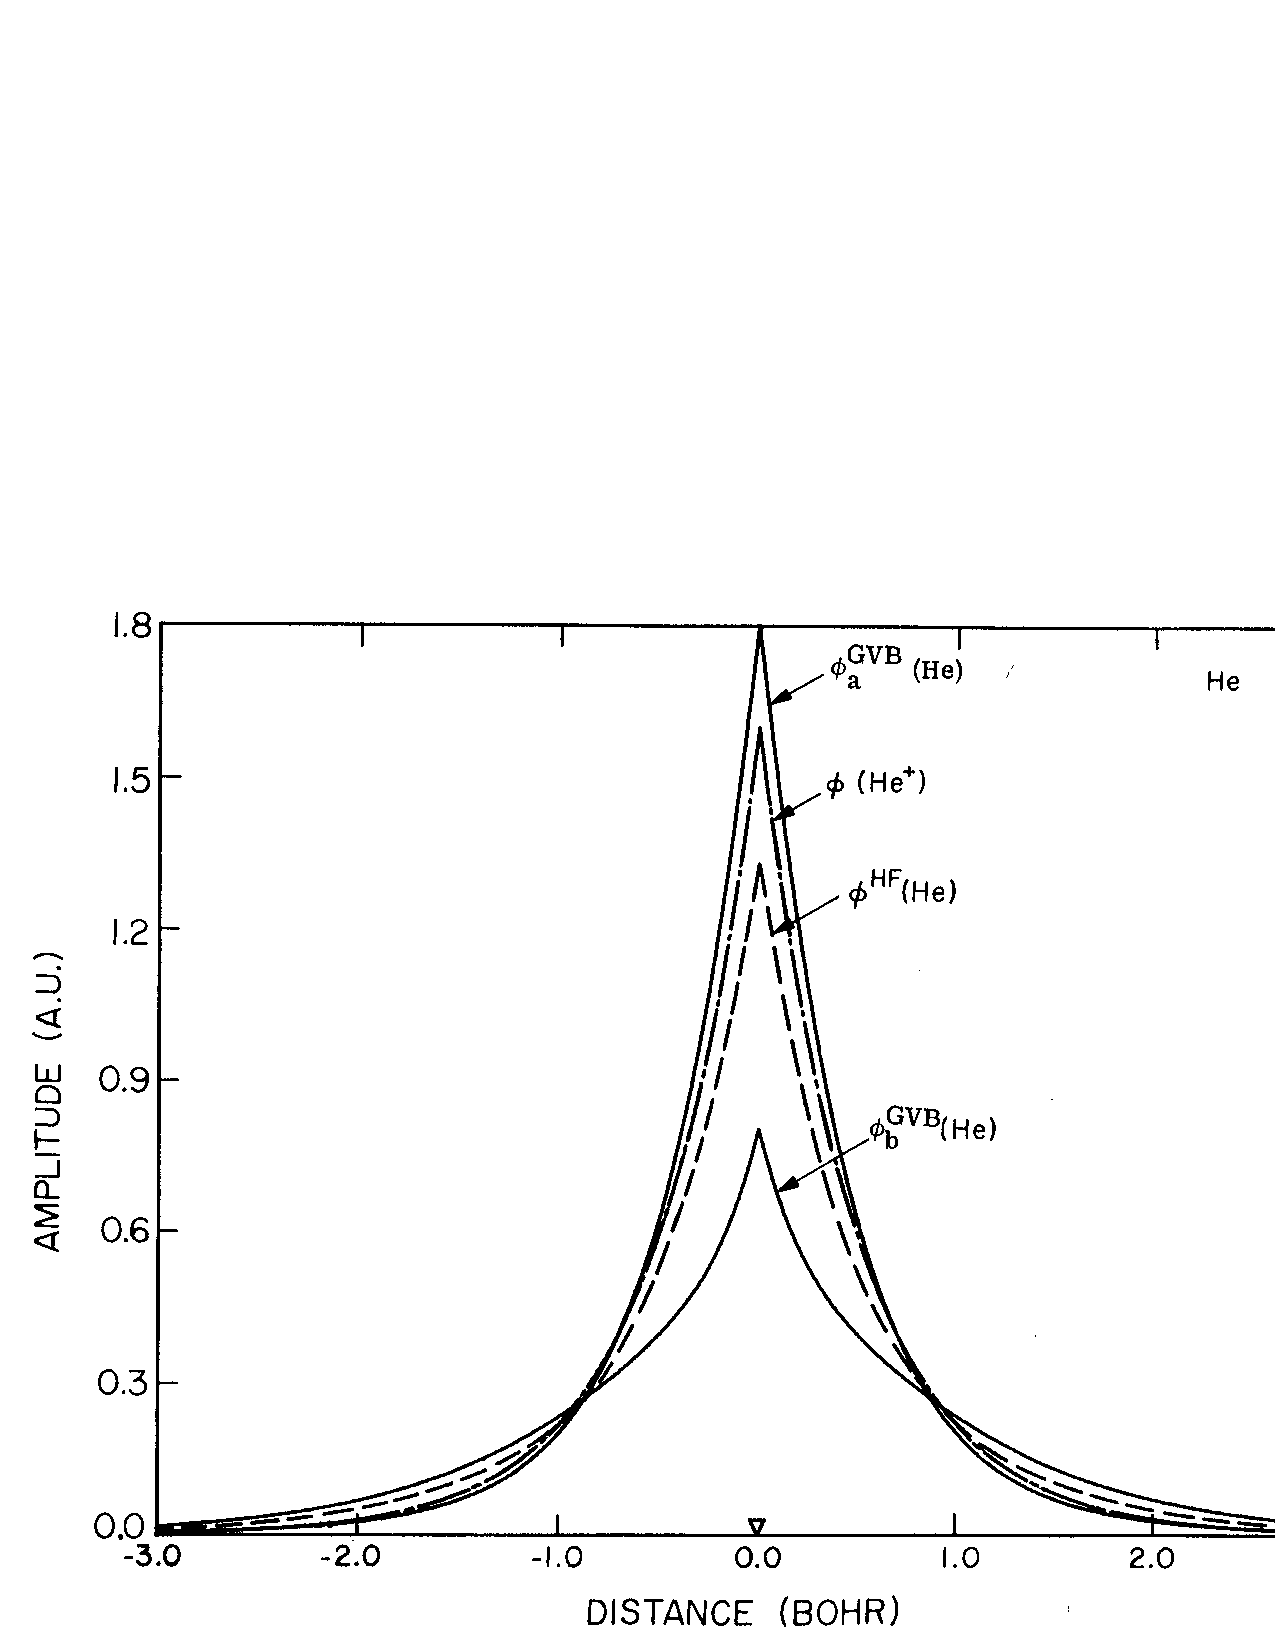
\includegraphics[scale=0.75]{fig3-13}
\caption{The HF and GVB orbitals for He and He$^+$.}
\label{fig3-14}
\end{figure}

We see that $\varphi^{GVB}_a$ is very similar to the $1s$ orbital of
He$^+$, and that $\varphi^{GVB}_b$ is much more diffuse.  Thus, we
envision He as having, first, one electron in the $1s$ orbital of
He$^+$ (this is orbital $\varphi_a$) experiencing an effective nuclear
charge of $Z \approx 2$, and secondly, the second electron in an
orbital ($\varphi_b$) experiencing an effective charge of $Z \approx
1$, nuclear charge of 2 but shielded by the $\varphi_a$ electron.
Describing both $\varphi_a$ and $\varphi_b$ as simple exponentials and
optimizing the exponents, leads to effective charges of $\zeta_b =
1.189$ and $\zeta_a =$ 2.183, as expected from the simple
picture \cite{chap3-ref15}.

This type of correlation is referred to as \emph{in-out correlation}
since when one electron is closer to the nucleus, the other tends to
be farther away.  This GVB picture is somewhat different from the HF
model, where both electrons are in the same orbital and one cannot
relate the description so simply to that of He$^+$.

A more extreme case is H$^-$, the GVB orbitals for which are shown in
Figure \ref{fig3-15}. Here, the first electron (in $\varphi_a$) is
very similar to a hydrogen $1s$ orbital, and the second electron is
barely bound, leading to a very diffuse $\varphi_b$ orbital.  As shown
in Tables \ref{table3-03a}-\ref{table3-03d}, the HF wavefunction of
H$^-$ yields an energy of $-$0.487, higher than the energy of the
hydrogen atom, implying that H$^-$ is not stable with respect to H
plus an electron.  The second electron cannot leave since the HF
orbital is doubly occupied.  Thus, either both electrons stay or both
leave. The GVB wavefunction yields an energy of $-$0.513, correctly
accounting for the stability of H$^-$, the exact energy is $-$0.527.

\begin{figure}
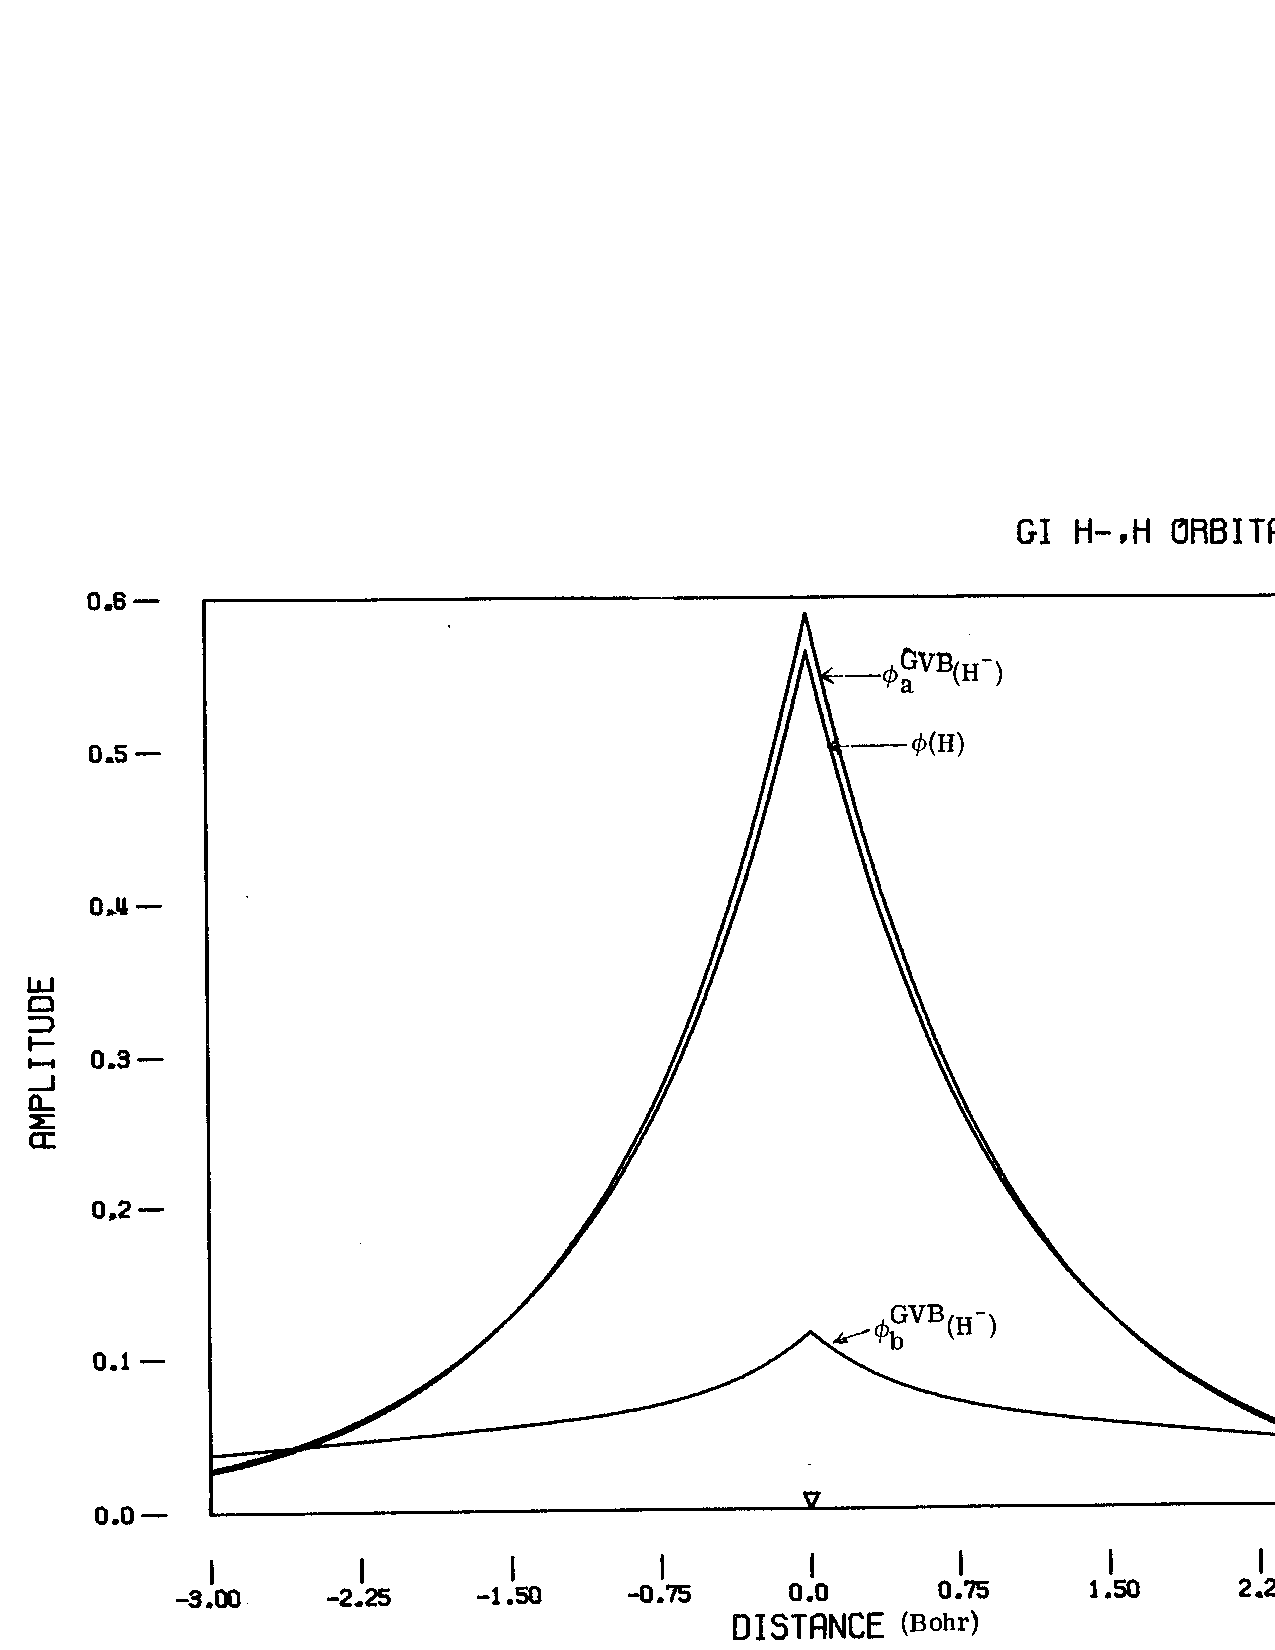
\includegraphics[scale=0.75]{fig3-14}
\caption{The GVB orbitals of H$^-$.  }
\label{fig3-15}
\end{figure}

\begin{table}
\caption{Comparison of energies for two-electron atoms: Exact.}
\label{table3-03a}
\begin{tabular}{ccc} \\ \hline
& $E^a$ & I.P.$^b$\cr
H$^-$ & $-$0.527751 & 0.027751\cr
He & $-$2.903724 & 0.903724\cr
Li$^+$ & $-$7.279914 & 2.779914\cr
Be$^{++}$ & $-$13.65557 & 5.65557\cr
B$^{3+}$ & $-$22.03097 & 9.53097\cr
C$^{4+}$ & $-$32.40625 & 14.40625\cr
N$^{5+}$ & $-$44.78145 & 20.28145\cr
O$^{6+}$ & $-$59.15660 & 27.15660\cr
F$^{7+}$ & $-$75.53171 & 35.03171\cr
Ne$^{8+}$ & $-$93.90681	& 43.90681\cr \hline 
\end{tabular}
\end{table}

\begin{table}
\caption{Comparison of energies for two-electron atoms. HF}
\label{table3-03b}
\begin{tabular}{ccccc} \\ \hline
& $E^c_{HF}$ & $\epsilon^C_{HF}$ & IP ($\Delta E$) & $E_{corr}$\cr
H$^-$ &$-$0.4870$^d$ &$-$0.0642$^d$ &$-$0.0130 & 0.0408\cr
He &$-$2.861680&$-$0.917956	& 0.8617 & 0.0420\cr
Li$^+$ &$-$7.2364150&$-$2.792365 & 2.7364 & 0.0435\cr
Be$^{++}$ &$-$13.61130&$-$5.667116 & 5.6113 & 0.0443\cr
B$^{3+}$ &$-$21.98623&$-$9.541979 & 9.4862 & 0.0447\cr
C$^{4+}$ &$-$32.36119&$-$14.41689 & 14.3612 & 0.0451\cr
N$^{5+}$ &$-$44.73616&$-$20.29183 & 20.2362 & 0.0453\cr
0$^{6+}$ &$-$59.11115&$-$27.166679 & 27.1112 & 0.0455\cr
F$^{7+}$ &$-$75.48613&$-$35.04176 & 34.9861 & 0.0456\cr
Ne$^{8+}$ &$-$93.86112&$-$43.91673 & 43.8611 & 0.0457\cr \hline 
\end{tabular}
\end{table}

\begin{table}
\caption{Comparison of energies for two-electron atoms: GVB.}
\label{table3-03c}

\begin{tabular}{cccccc} \\ \hline
& $E_{GVB}$ & $\epsilon_a$ & $\epsilon_b$ & IP ($\Delta E$) & $E_{corr}$\cr
H$^-$&$-$0.51384$^d$&$-$0.26800&$-$0.01471&0.0138&0.0139\cr
He&$-$2.87800$^f$&$-$1.2152&$-$0.9039&0.8780&0.0257\cr
Li$^+$ &$-$7.25142$^f$&$-$3.1965&$-$2.8149&2.7514&0.0285\cr
Be$^{++}$ &$-$13.62577$^f$&$-$6.1746&$-$5.7330&5.6258&0.0298\cr
B$^{3+}$ &$-$22.000159&$-$10.14932&$-$9.65472&9.5002&0.0308\cr
C$^{4+}$ & & & & & \cr
N$^{5+}$ & & & & & \cr
0$^{6+}$ & & & & & \cr
F$^{7+}$ & & & & & \cr
Ne$^{8+}$& & & & & \cr \hline
\end{tabular}
\end{table}


\begin{table}
\caption{Comparison of energies for two-electron atoms: CI.}

\label{table3-03d}
\begin{tabular}{ccc} \\ \hline
& $E^e_{CI}$ \cr
H$^-$ & $-$0.52751\cr
He & $-$2.90320\cr
Li$^+$ & $-$7.27924\cr
Be$^{++}$ & $-$13.65481\cr
B$^{3+}$ & $-$2.03016\cr
C$^{4+}$ & $-$32.40540\cr
N$^{5+}$ & $-$44.78057\cr
0$^{6+}$ & $-$59.15570\cr
F$^{7+}$ & -\cr
Ne$^{8+}$ & -\cr \hline

\end{tabular} \\
$^a$See reference 21.  $^b$Calculated using $E$ from reference 21. 
$^c$See reference 20.  $^d$See reference 22. $^e$See reference 23. 35
configurations were used. $^f$See reference 24. $^g$See reference 25.
\end{table}


\subsection{CI Wavefunctions for the He Atom}

The results of several CI calculations on He are shown in Table
\ref{table3-04}. Analyzing in terms of natural orbitals leads to the
results in Table \ref{table3-05}.  Here we see that the $2s$, $2p_x$,
$2p_y$, and $2p_z$ natural orbitals provide the dominant electron
correlation effects.  These are the only natural orbitals containing
just one nodal plane.  Plots of the $2s$ and $2p$ natural orbitals are
given in Figure \ref{fig3-16}, where we see that the higher natural
orbitals are concentrated in the same region as the $1s$ orbital but
with the additional nodal plane, circular for $\psi_{2s}$ and planar
for each $\varphi_{2p}$.

\begin{figure}
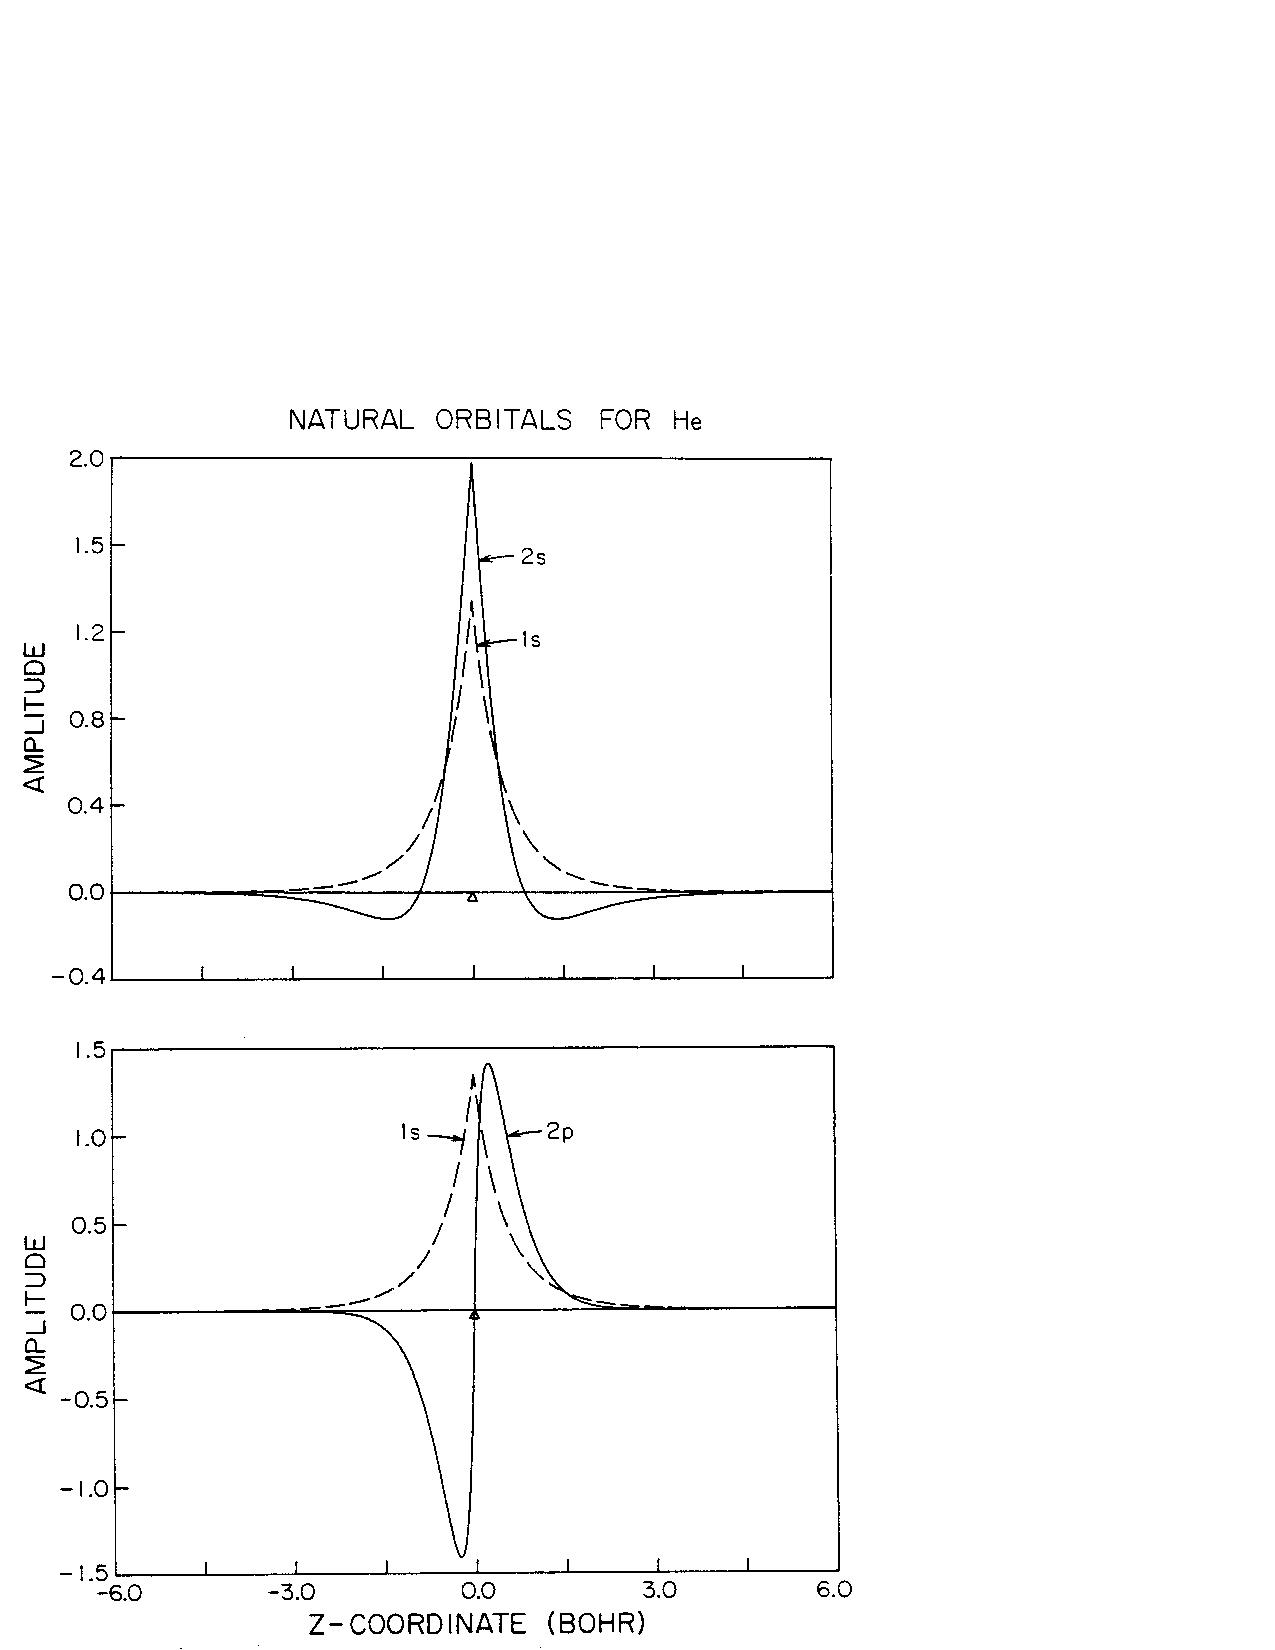
\includegraphics[scale=0.75]{fig3-15}
\caption{The natural orbitals for He.}
\label{fig3-16}
\end{figure}

\begin{table}
\caption{Energies for CI wavefunctions 
of the ground state of He atom.}
\label{table3-04}
\begin{tabular}{cccccc} \\ \hline
\multicolumn{5}{c}{Number of Basis Functions$^a$} & Energy\cr
s & p & d & f & g \cr \hline

5 & & & & & $-$2.87896$^a$\cr
5 & 4 & & & & $-$2.90039$^a$\cr
5 & 4 & 3 & & & $-$2.90258$^a$\cr
5 & 4 & 3 & 2 & & $-$2.90307$^a$\cr
5 & 4 & 3 & 2 & 1 & $-$2.90320$^a$\cr
Pekeris & & & & & $-$2.90372$^b$\cr
HF & & & & & $-$2.86168\cr
GVB & & & & & $-$2.87800\cr\hline
\end{tabular}\\
$^a$See reference 23.  $^b$See reference 26.
\end{table}

\begin{table}
\caption{Analysis of He CI wavefunction 
in terms of natural orbitials.$^a$}
\label{table3-05}

\begin{tabular}{ccc} \\ \hline
Natural Orbital & Energy Lowering (mh) & \% $E_{corr}$\cr
$2s$ & 16.30 & 38.83\cr
$2p$ & 	19.51 & 46.46\cr
$3s$ & 	0.88 & 2.09\cr
$3p$ &	1.63 & 3.87\cr
$3d$ &	1.80 & 4.28\cr
$4s$ &	0.09 & 0.22\cr
$4p$ &	0.26 & 0.62\cr
$4d$ &	0.36 & 0.86\cr
$4f$ &	0.35 & 0.83\cr
Totals & 41.18 & 98.05\cr \hline
\end{tabular}\\
$^a$See reference 27.  $^b$Total correlation energy is equal to 0.0420 hartree.
\end{table}

Using the five dominant natural orbitals, $1s$, $2s$, $2p_x$, $2p_y$, and 
$2p_z$, leads to the wavefunction
\begin{equation}
\psi^{CI} = C_{1s} \varphi_{1s} \varphi_{1s} - C_{2s} \varphi_{2s} \varphi_{2s} - 
C_{2p} \left[ \varphi_{2p_x} \varphi_{2p_x} + \varphi_{2p_y} \varphi_{2p_y} + 
\varphi_{2p_x} \varphi_{2p_x}\right]
\label{chap3-eqno62}
\end{equation}
where $C_{1s} = 0.99599$, $C_{2s} = 0.06160$, and $C_{2P} = 0.06188$.
This wavefunction has an energy of $-2.8975$, just 0.17 eV above the
exact, nonrelativistic, energy of $-$2.9037.  This wavefunction is
sufficiently accurate that, for the purposes of this course, we will
consider (\ref{chap3-eqno62}) as the exact wavefunction of He.

\subsubsection{CI Wavefunction Interpretation}

To interpret the wavefunction (\ref{chap3-eqno62}), we will consider
one by one the effects of adding any one of the four correlating terms
to the dominant, first, term.  The wavefunction
\begin{equation}
C_{1s} \varphi_{1s} \varphi_{1s} - C_{2s} \varphi_{2s} \varphi_{2s}
\label{chap3-eqno63}
\end{equation}
can be rewritten in the GVB form
\begin{equation}
\varphi_a \varphi_b + \varphi_b \varphi_a
\label{chap3-eqno64}
\end{equation}
where
\begin{equation}
\sqrt{2} \varphi_a = \sqrt{C_{1s}} \varphi_{1s} + \sqrt{C_{2s}} \varphi_{2s}
\end{equation}
\begin{equation}
\sqrt{2} \varphi_b = \sqrt{C_{1s}} \varphi_{1s} - \sqrt{C_{2s}} \varphi_{2s}
\end{equation}
are the GVB orbitals.  Thus, from earlier in this section, we see that
the $\varphi_{2s}$ natural orbital in (\ref{chap3-eqno63}) builds in
radial correlation, increasing the probability of the second electron
being at larger $r$ when the first electron is at smaller $r$, and
vice versa.

Similarly the wavefunction
\begin{equation}
C_{1s} \varphi_{1s} \varphi_{1s} - C_{2p} \varphi_{2p_x} \varphi_{2p_x}
\end{equation}
can also be rewritten as (\ref{chap3-eqno64}), where
\begin{equation}
\sqrt{2} \varphi_a = \sqrt{C_{1s}} \varphi_{1s} + \sqrt{C_{2p}} 
\varphi_{2p_x}
\label{chap3-eqno65a}
\end{equation}
\begin{equation}
\sqrt{2} \varphi_b = \sqrt{C_{1s}} \varphi_{1s} - \sqrt{C_{2p}} 
\varphi_{2p_x}
\label{chap3-eqno65b}
\end{equation}
In (\ref{chap3-eqno65a})--(\ref{chap3-eqno65b}) we see that when one
electron is in the $+x$ direction, the other tends to be in the $-x$
direction.  Similar results occurs for the $\varphi_{2p_y}$ and
$\varphi_{2p_z}$ terms.  The three correlations resulting from the
terms involving $p$ orbitals, are grouped together and referred to as
\emph{angular correlation}.

The three terms of (\ref{chap3-eqno62}) involving $p$ orbitals, can be
written as
\begin{eqnarray}
\left[ \varphi_{2px} \varphi_{2px} + \varphi_{2py} \varphi_{2py} + \varphi_{2pz} 
\varphi_{2pz} \right] &=& R(1)R(2) [\sin \theta_1 \cos \varphi_1 
\sin \theta_2 \cos \varphi_2 \\ \nonumber
 && + \sin \theta_1 \sin \varphi_1 \sin 
\theta_2 \sin \varphi_2 + \cos \theta_1 \cos \theta_2 ]\\
&=& R_{2p} (1) R_{2p} (2) \cos \theta_{12} ,
\end{eqnarray}
where $R(i)$ is the radial part of the orbital $\varphi_i$, and
$\theta_{12}$ is the angle between electron 1 and electron 2.
Combining with the first term of (\ref{chap3-eqno62}), we obtain
\begin{equation}
C_{1s} R_{1s} (1) R_{1s} (2) - C_{2p} R_{2p} (1) R_{2p} \cos 
\theta_{12} .
\label{chap3-eqno66}
\end{equation}
With this form, we see that the magnitude of the wavefunction is
increased (with respect to $\varphi_{1s} \varphi_{1s}$) for $|
\theta_{12} | > 90^{\circ}$ and decreased for $| \theta_{12} | >
90^{\circ}$.  Thus, (\ref{chap3-eqno66}) effects an angular
correlation of the electrons.

Each of the four dominant correlating orbitals has one nodal plane not
contained in $\varphi_{1s}$, and the correlation effect is across the
nodal plane, increased probability of electrons being on opposite
sides.  Of course, $\varphi_{1s}$ has no nodal planes, however, we
have worded this so as to be appropriate also for correlations of more
complicated orbitals than $\varphi_{1s}$.  Starting with the
$\varphi_{1s}$ orbital, there are just four possible orbitals
orthogonal to $\varphi_{1s}$ but containing a single nodal plane,
namely the above four.  All additional correlating terms will involve
two or more nodal planes, leading to higher energies, and all are
relatively unimportant, leading to a total energy contribution of 6.2
mh = 0.17 eV = 3.9 kcal.  For the purposes of most of our
considerations of molecules, an energy error of 0.1 eV is acceptable,
and we will completely ignore these smaller terms.  Thus, we will
consider (\ref{chap3-eqno62}) as the CI wavefunction of He.

\section{Wavefunctions of H$_2$}

In this section we will discuss the HF, GVB, 
and CI wavefunctions for H$_2$.

\subsection{HF Wavefunctions for H$_2$}

In Figure \ref{fig3-17}, we show how quickly the HF
wavefunctions for H$_2$ converge as a function of basis set size, $P$.
The major effects in the orbital shape are in the bond region.

\begin{figure}
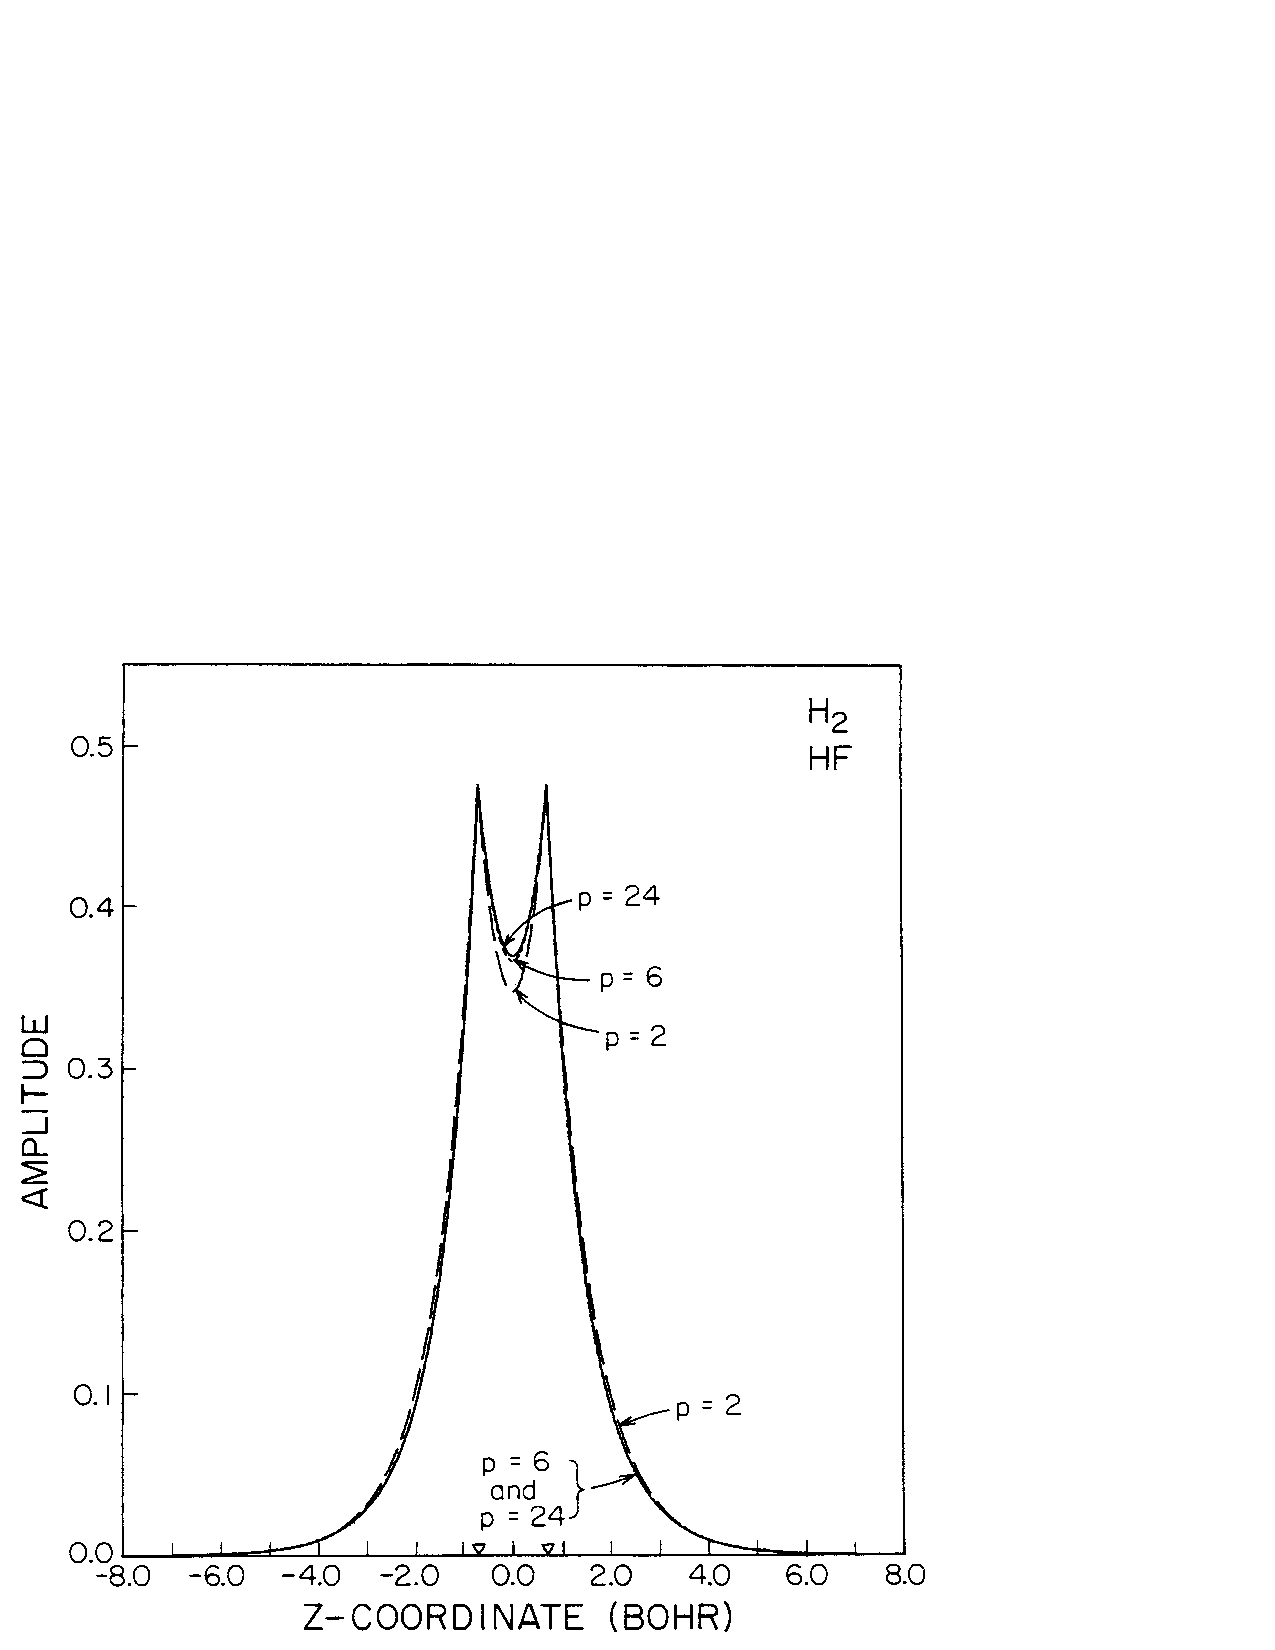
\includegraphics[scale=0.75]{fig3-16}
\caption{HF wavefunctions for H$_2$ with $R = 1.4a_0$. $p$
indicates the number of functions in the basis set.}
\label{fig3-17}
\end{figure}

In Figure \ref{fig3-18}, we compare the MO wavefunction ($P = 2$,
$\zeta = 1$) with the MBS wavefunction ($P =2$, $\zeta_{OPT}$).  Here
there are significant changes near the nuclear and bond regions.

\begin{figure}
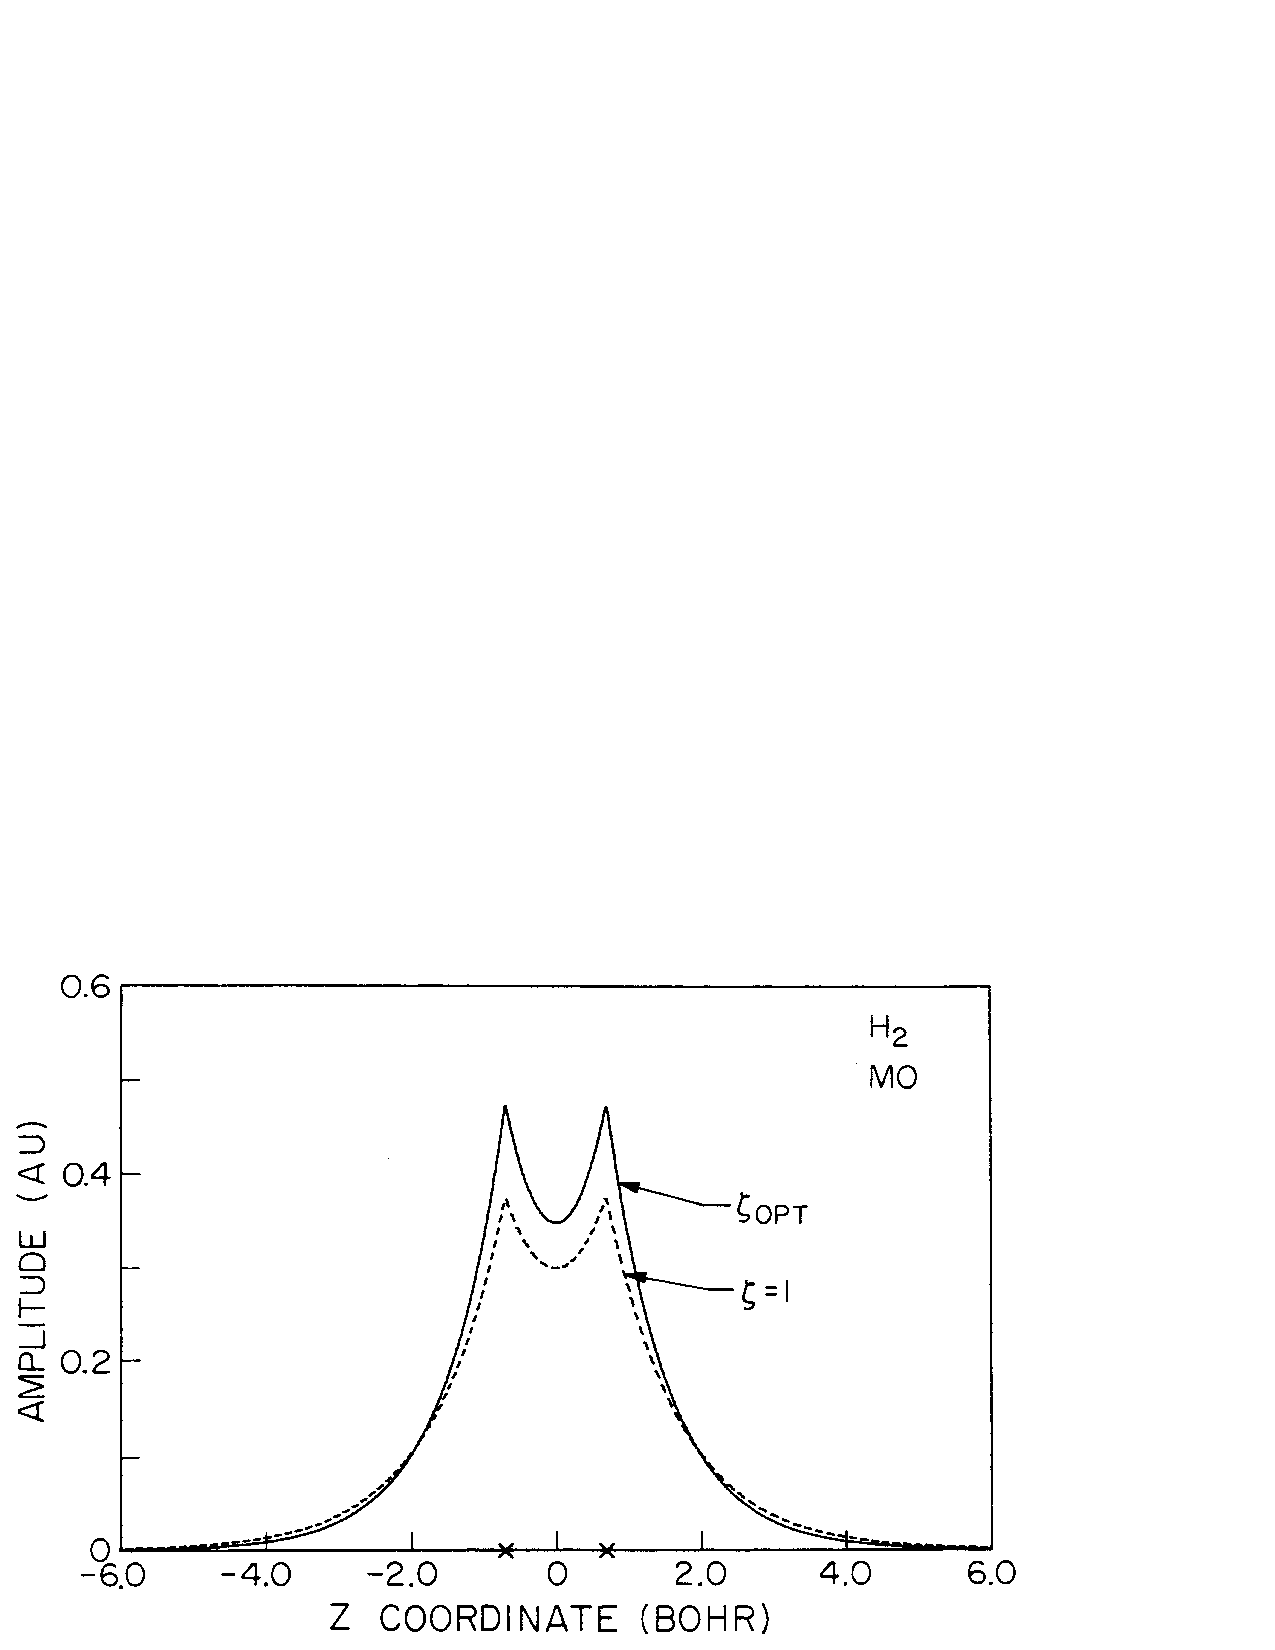
\includegraphics[scale=0.75]{fig3-17}
\caption{MO for H$_2$ using $\zeta = 1$, and $\zeta_{OPT} = 1.1895$ 
($R = 1.4a_0$).} 
\label{fig3-18}
\end{figure}

Comparing the energies in Table \ref{table3-06}, we see that $P = 6$
leads to an energy within 0.00152 h = 0.04 eV = 1 kcal of the HF
limit.  We consider this as a good level of accuracy.  The $P = 6$
basis has two (optimized) $s$ functions on each H and an (optimized)
$p$ function on each H.  Such a basis is referred to as \emph{double
valence} (for the two sets of $s$ functions) \emph{plus polarization}
(for the $p$ functions) and will be denoted as $DVP$.  More
commonly, double valence is referred to as double zeta.

\begin{table}
\caption{Energy quantities for HF wavefunctions of 
H$_2$ at $R = 1.4a_0$.  Only the coefficients on one atom are
shown, the others are equal by symmetry.}
\label{table3-06}

\begin{tabular}{cccccc} \\ \hline
P & 2 & 6$^a$ & 12$^b$ & 18$^b$ & 24$^b$ \cr
$E$ & $-$1.12819 & $-$1.13211 & $-$1.13353& $-$1.13359 & $-$1.13363\cr
$\epsilon$ & & $-$0.59443 & $-$0.59463& $-$0.59466 & $-$0.59465 \cr \hline

& $1s$(1.1895) 0.54572 & $1s$(1.378) 0.43262 & $1s$(1.19494) 1.03449
& $1s$(1.14615)	0.84994	& $1s$(1.18863)	0.90374 \cr

& & $2s$(1.176) 0.12384 & $1s$(3.22156) $-$0.6316
& $1s$(3.01720) $-$0.01359 & $1s$(2.50021) $-$0.04978\cr

& & $2p_x$(1.820) 0.02827 & $2s$(1.75027) $-$0.22058
& $2s$(O.77682)	0.00894	& $2s$(O.79445)	0.01144\cr

& & & 2s(3.41729) $-$0.02034
& $2s$(1.62362) $-$0.12071 & $2s$(1.73027) $-$0.12832\cr

& & & $2p_z$(1.81344) 0.04007
& $3s$(3.54949)	0.00753	& $3s$(3.43600)	0.00194\cr

& & & $2p_z$(3.55649) $-$0.00009
& $2p_z$(0.98920)	0.08858	& $2p_z$(1.05529)	0.03984\cr

&&&& $2p_z$(3.11550)	0.00273	& $2p_z$(1.98553) 	0.02413\cr
&&&& $3p_z$(3.80593) 0.00790	& $2p_z$(4.08182) $-$0.00094\cr
&&&& $3d_{z^2}$(l.19687) 0.02029	& $3p_z$(3.43359) 0.00129\cr
&&&& & $3d_{z^2}$(1.26663) 0.00649\cr
&&&& & $3d_{z^2}$(2.68042) 0.00393\cr
&&&& & $4f_{z^3}$(2.70808) 0.00103\cr\hline
\end{tabular} \\
$^a$See reference 28.  $^b$See reference 29.  Each basis function is 
normalized to $2/\sqrt{2}$.
\end{table}

With even the best of these HF wavefunctions, the energy is
0.04081 h = 1.1 eV above the exact, nonrelativistic, energy of H$_2$,
about the same as the correlation error of He, and other two-electron
ions. The HF potential curve, using the $P = 6$ basis of
Table \ref{table3-06}, optimized at each R but restricted so that
$\zeta_{1s} = \zeta_{2s}$, is shown in Figure \ref{fig3-19}.

\begin{figure}
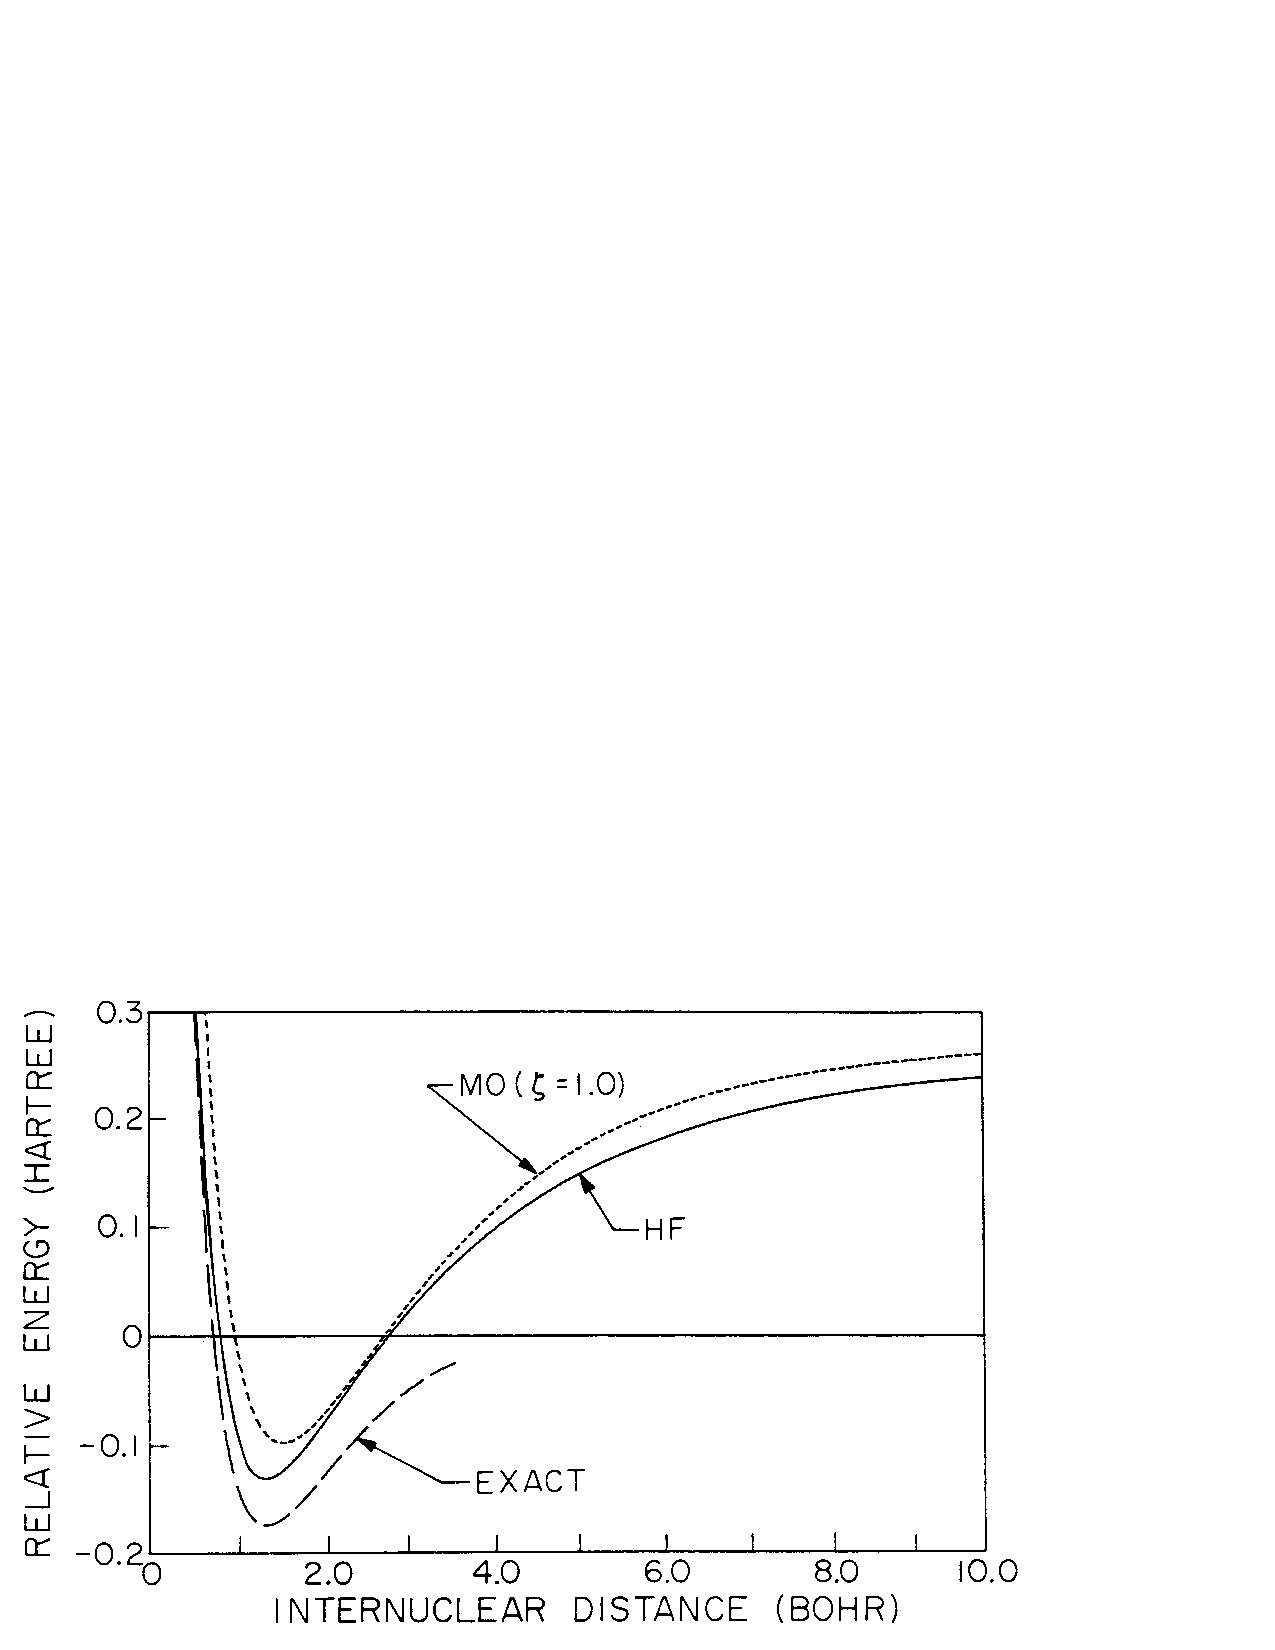
\includegraphics[scale=0.75]{fig3-18}
\caption{Comparison of energies for the MO wave function ($\zeta =
1.0$) and the HF wavefunction (six basis functions).}
\label{fig3-19}
\end{figure}

Just as with the MO wavefunction, the HF wavefunction at large $R$
leads to very serious errors.  Thus, at $R = 6\ a_0$, with the $P = 6$
wavefunction, the energy is $E = -0.82199$ (already far above the
dissociation limit $E = -1.0$) and the orbital energy is $\epsilon =
-0.32170$ (way off from the correct value at large $R$, $\epsilon =
-0.50$).  For $R = \infty$, the HF wavefunction leads to an energy of
$-$0.71542 which is 7.744 eV above the dissociation limit
\cite{chap3-ref16}.

\subsection{The GVB Wavefunction for H$_2$}

The GVB wavefunctions and energies for several optimized basis sets
are given in Table \ref{table3-07}.  A quite adequate description (0.2
kcal for the limit) is obtained using a single optimized $s$ function
and a single $p_z$ function on each center.  Even the MBS is only 4.1
mh = 0.11 eV above the limit.

\begin{figure}
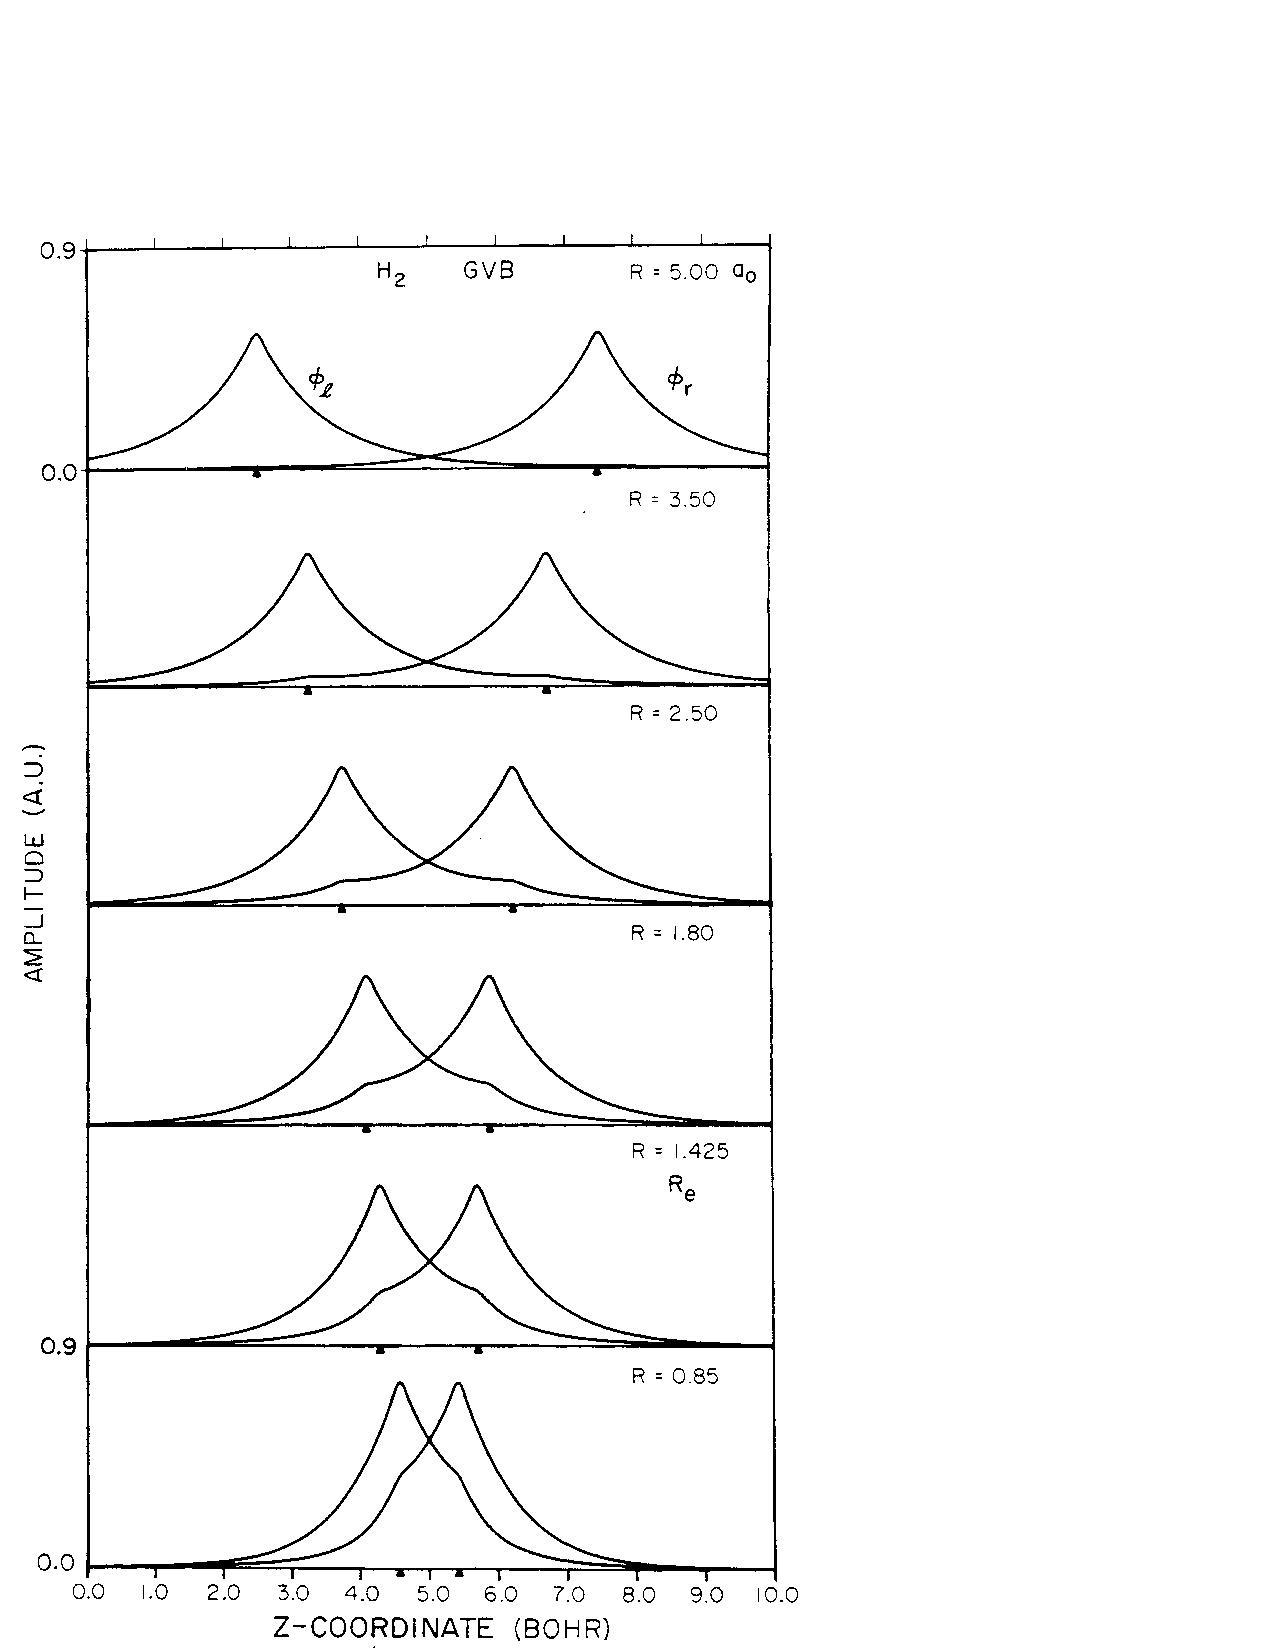
\includegraphics[scale=0.75]{fig3-19}
\caption{The GVB orbitals as a function of $R$. Note the cusps at the
nuclei have disappeared due to use of Gaussian basis functions.}
\label{fig3-20}
\end{figure}

\begin{table}
\caption{Energy and wavefunctions for GVB 
calculations on H$_2$ at $1.4a_0$.  Only the $\varphi_\ell$ orbitals is given, 
the $\varphi_r$ orbital is the mirror image.  The same basis occurs on both 
centers with the orbitals on the left first, the
basis functions on the right have no exponent listed. A $p_z$ basis function
with plus coefficient is positive toward the second center.  All quantities 
in hartree atomic units.}
\label{table3-07}
\begin{tabular}{cccc}\\\hline
P & 2 & 4$^a$ & 6$^b$\cr
E & $-$1.147777 & $-$1.151345 & $-$1.151526\cr
$\epsilon$ & $-$0.6877&$-$0.68348&$-$0.68472\cr \hline
S & 0.79700	& 0.80093 & 0.80420\cr
ns$(\zeta)C_{\mu}$&1s(1.2005) 0.91287&1s(1.1909)0.8890&1s(1.3129) 0.77499\cr
& 1s         0.12303&$2p_z$(2.0928)$-$0.00672&2s(1.1566) 0.11116\cr
& & 1s         0.13631&$2p_z$(1.9549)$-$0.00310\cr
& & $2P_z$        0.03006	&$1s$          0.12161\cr
& & & $2s$          0.04199\cr
& & & $2p_z$         0.03769\cr \hline
\end{tabular}\\
$^a$Using $1s(1.262)$ and $2s(1.191)$ basis functions on each center, 
leads to $E = -1.147804$.  $^b$Using $1s(1.3092), 2s(1.1273), 2p_z(1.700)$, 
and $3d^2_z(2.37)$ basis functions on each center, leads to $E = -1.151887$.
\end{table}

At large $R$ the orbitals are atomic-like, but for smaller $R$, the
GVB orbital gradually becomes more contracted about each nucleus.
These readjustments in the orbitals are such that the contragradience
in the bond region is about the same as for the VB
wavefunction.  From 1 to $6\ a_0$, the GVB orbitals leads to a much
greater overlap than the VB orbital, as shown in Figure
\ref{fig3-21}.  For example, at $R = 1.4\ a_0$, $S^{GVB} = 0.804$ as
compared to $S^{VB} = 0.753$.

\begin{figure}
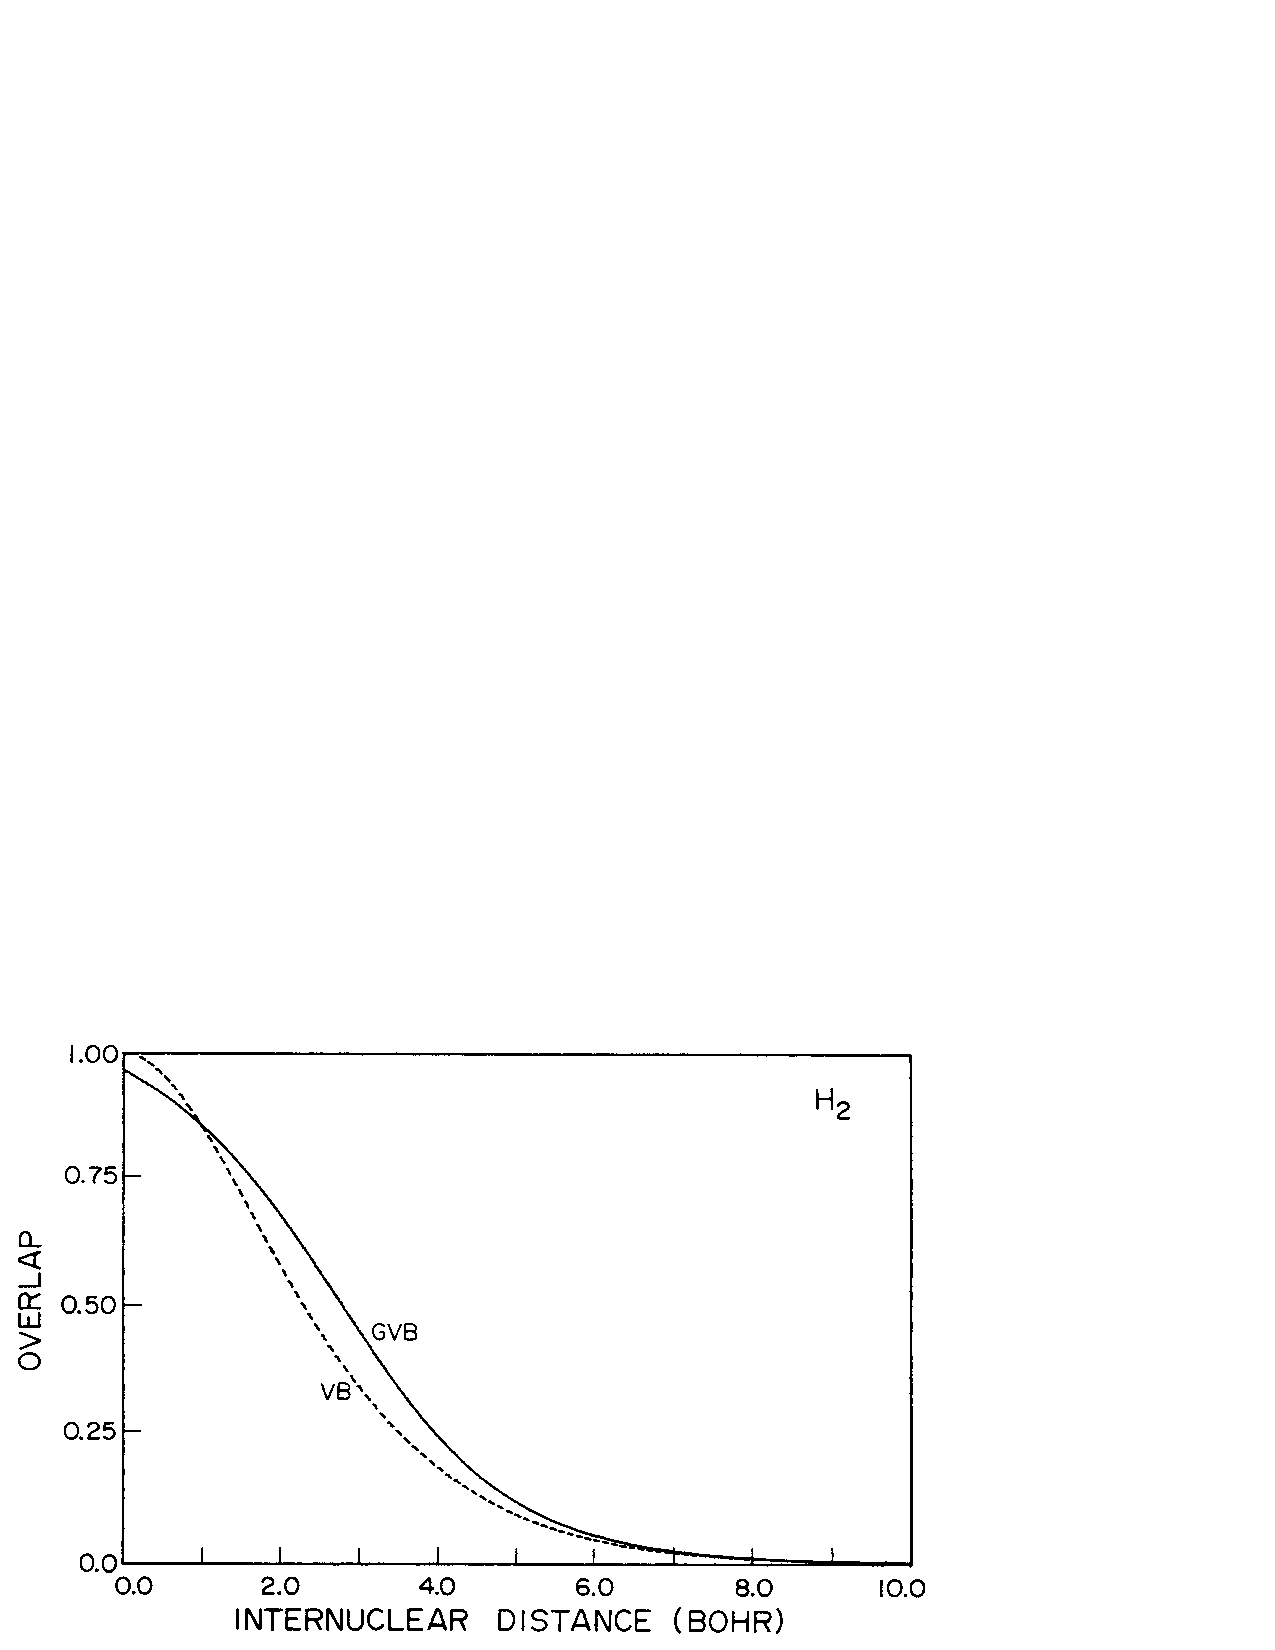
\includegraphics[scale=0.75]{fig3-20}
\caption{Comparison of overlap, $S = \langle \varphi_\ell 
\vert \varphi_r \rangle$ for the VB and GVB wave functions.}
\label{fig3-21}
\end{figure}

\subsubsection{Energy Analysis}

The GVB orbitals of H$_2$ are compared with the
VB orbitals in Figure \ref{fig3-22}, where we see that the
orbitals readjust in such a way as to maintain the large
contragradience in the bond region, while concentrating the orbitals
more about each nucleus.

\begin{figure}
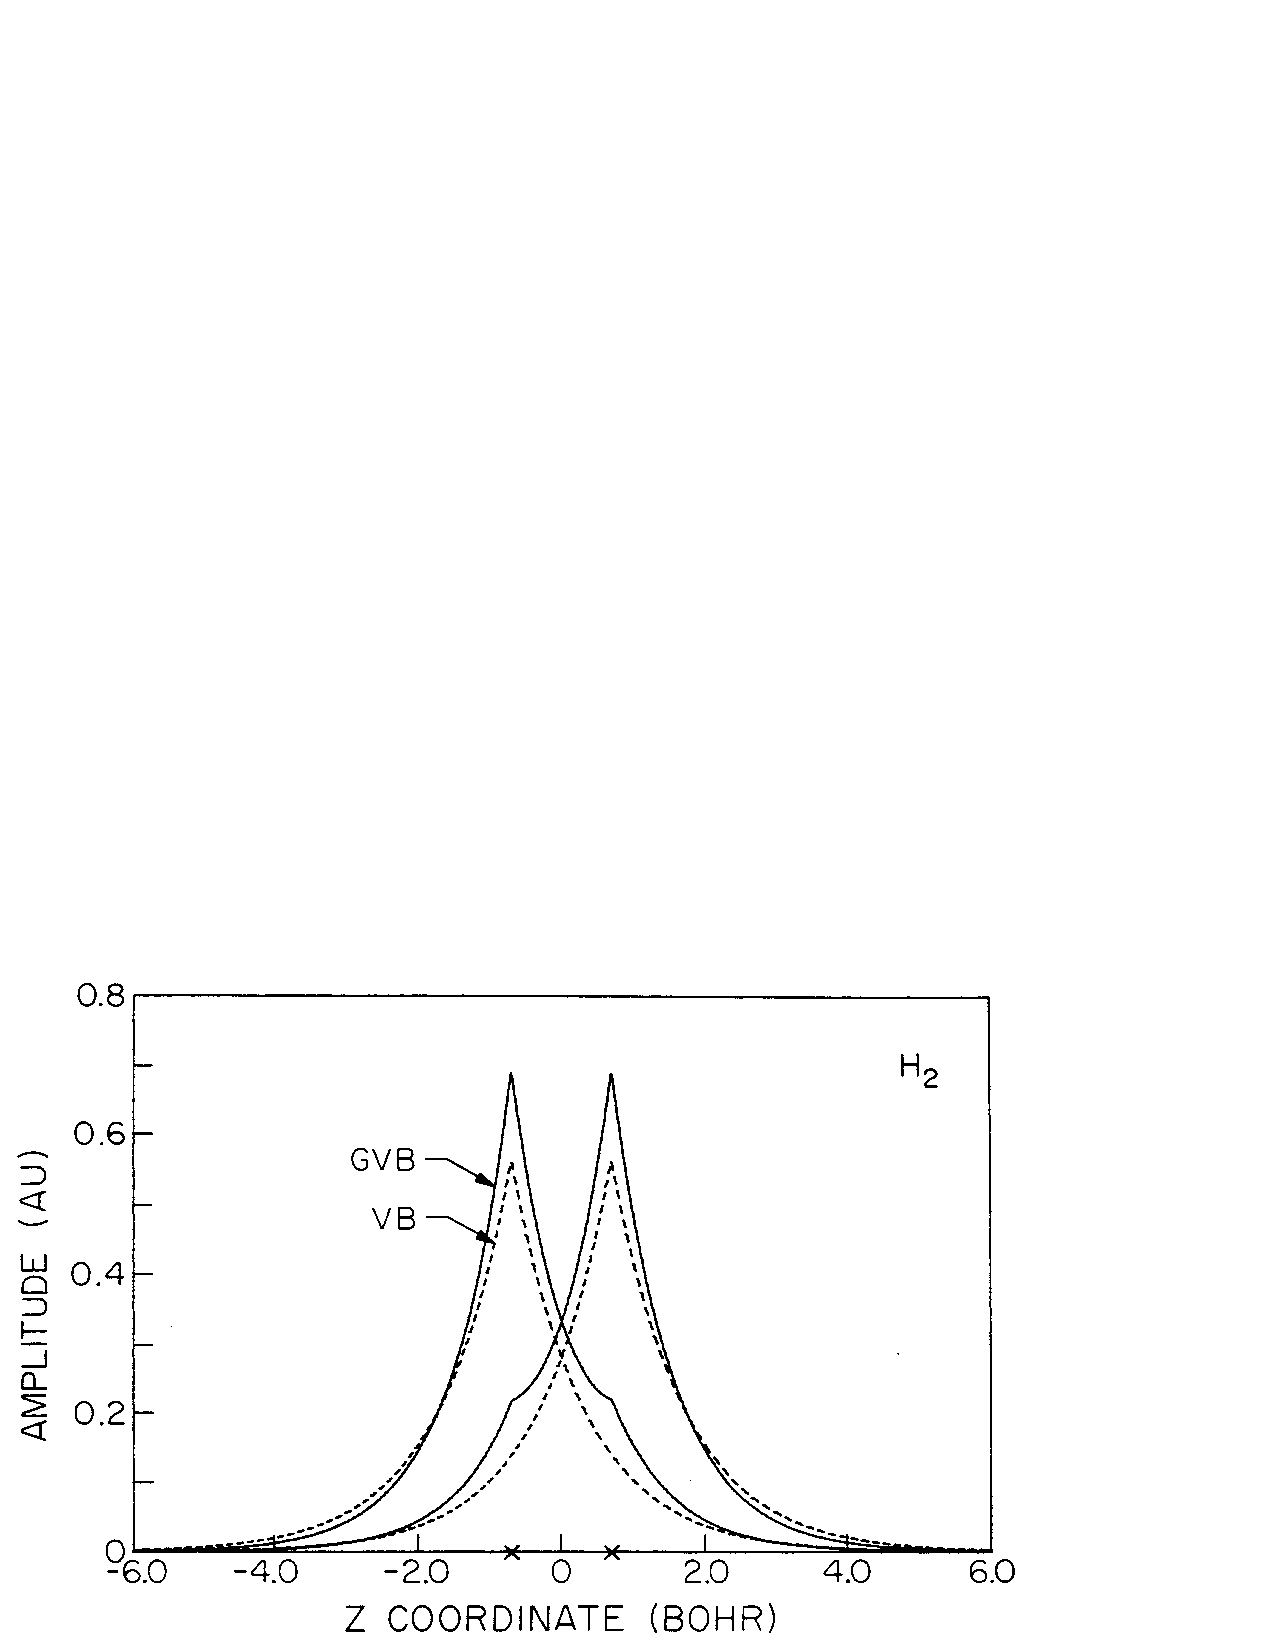
\includegraphics[scale=0.75]{fig3-21}
\caption{Comparison of GVB (two basis functions, $\zeta_{OPT} =
1.2005$) and VB ($\zeta = 1$) orbitals for H$_2$, $R = 1.4a_0$.}
\label{fig3-22}
\end{figure}

The GVB energy curves are compared with other
energy curves in Figure \ref{fig3-23}.

\begin{figure}
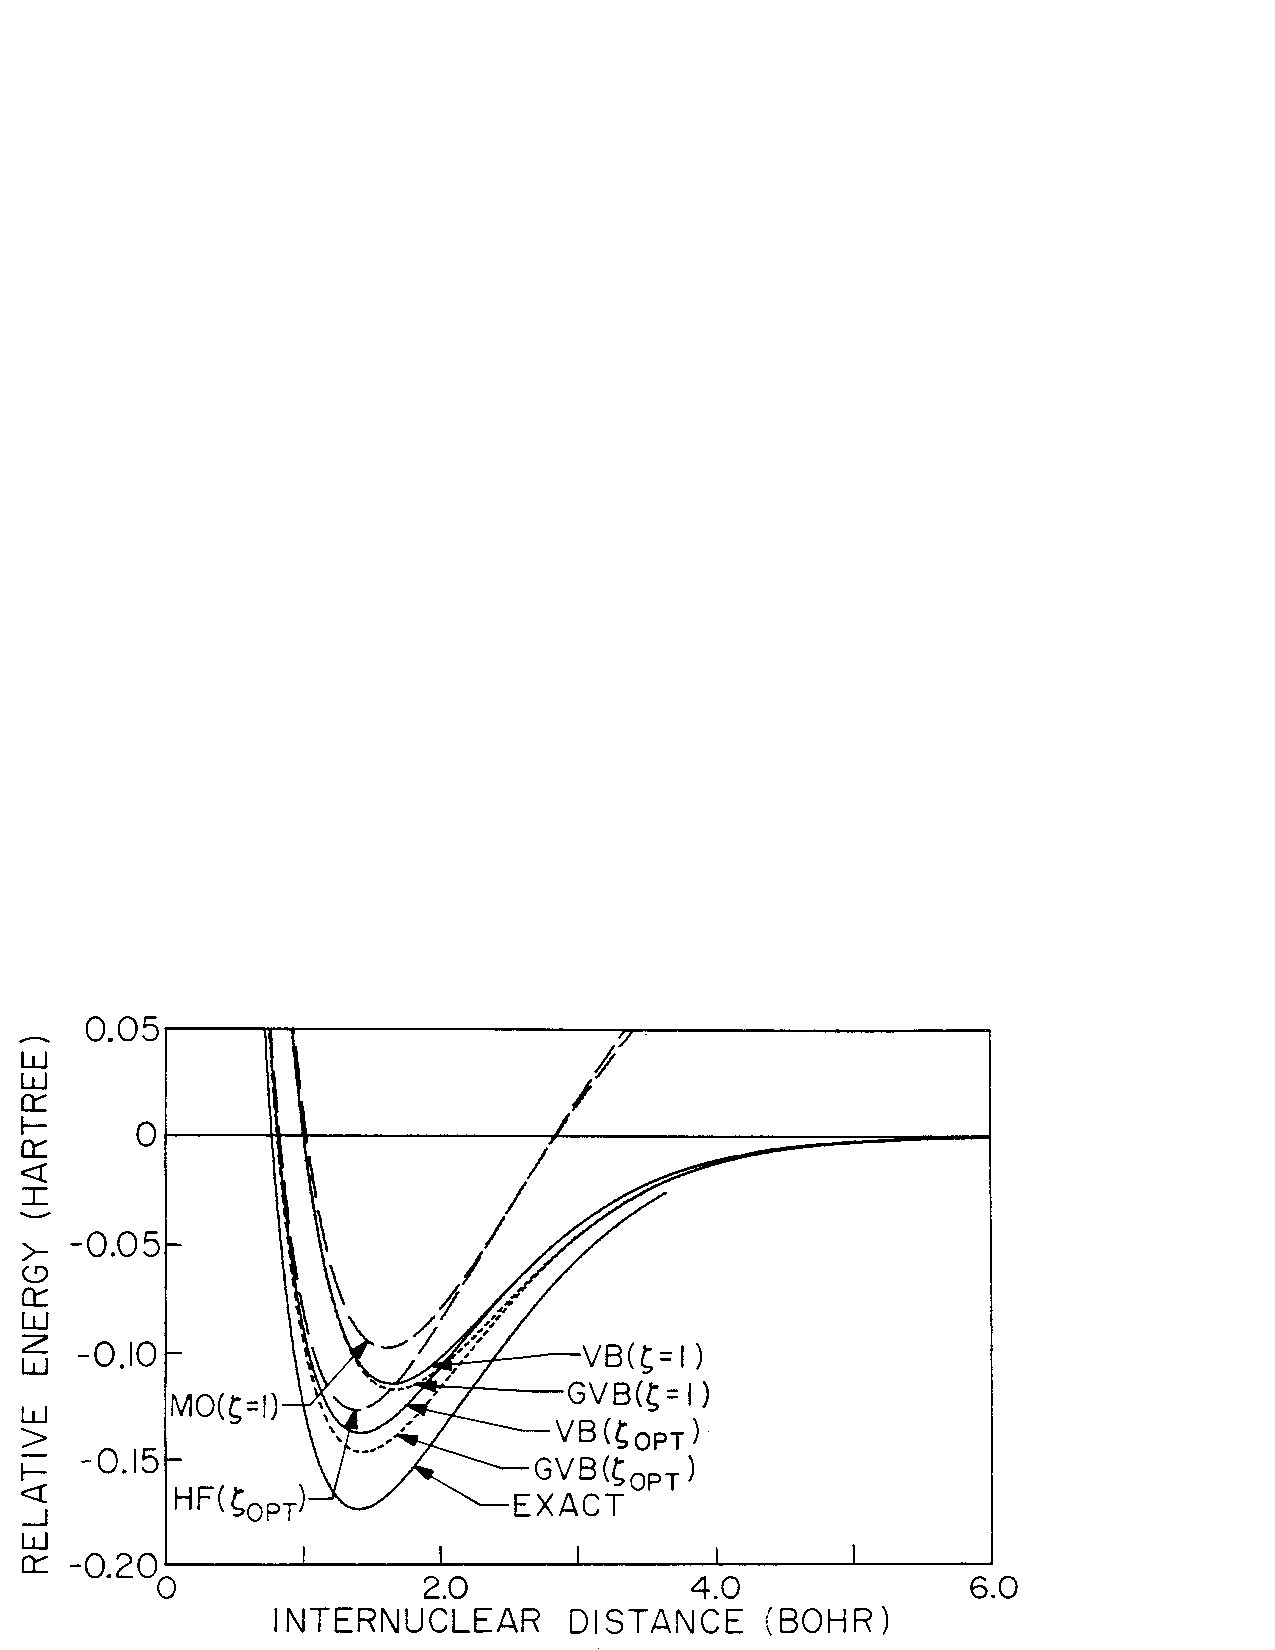
\includegraphics[scale=0.75]{fig3-22}
\caption{Comparison of the energy curves for MO, HF, VB, and GVB
wave functions of H$_2$. Only two basis functions were used for HF and
GVB. The results for both $\zeta = 1$ and  
$\zeta_{OPT}$ are shown.  The $\zeta_{OPT}$ as a function of $R$ are given 
in Figure \ref{fig3-24} later. The energy is relative to the energy
of two hydrogen atoms.}
\label{fig3-23}
\end{figure}

Some of the energy parameters of the HF, VB, and
GVB wavefunctions are compared in Table
\ref{table3-08}, while the $\zeta_{OPT}$ as a function of $R$, is
given in Figure \ref{fig3-24}.

\begin{figure}
% Warning: fig3-23 is missing!
%\includegraphics[scale=0.75]{fig3-23}
\caption{$\zeta_{OPT}$ for HF, VB and GVB wave functions.}
\label{fig3-24}
\end{figure}

\begin{table}
\caption{Comparison of results on H$_2$ for approximate wavefunctions 
using two basis functions.  All quantities are in atomic units; the energies 
are relative to two hydrogen atoms at $R = \infty$.}
\label{table3-08}
\begin{tabular}{cccccc} \\ \hline

& & HF & VB & GVB & Exact\cr
$\zeta = 1.0$ & $R_e$ & 1.603 & 1.643 & 1.668\cr
& $E_e$ & $-$0.0990808 & $-$0.115971 & $-$0.118651\cr
$\zeta_{OPT}$ & $R_e$ & 1.385 & 1.414 & 1.431 & 1.401\cr
& $E_e$ & $-$0.128231 & $-$0.139083& $-$0.147938 & $-$0.174470\cr
& $\zeta_{OPT}$ & 1.1931 & 1.1661	& 1.1937 & -\cr
$R = 1.4a_0$ & $E$ & 
$-$0.128189&$-$0.139049&$-$0.147777&$-$0.174470\cr
& $\zeta_{OPT}$ & 1.1895 & 1.1695 & 1.2005\cr \hline
\end{tabular}
\end{table}

\noindent
For $\zeta = 1.0$, all three wavefunctions yield an $R_e$ for too
large, 14\% to 19\%.  Optimizing $\zeta$ leads to errors of only 1\%
to 2\% in $R$, and improves the calculated bond energies by about
20\%.  It is characteristic that GVB leads to too large an $R$, while
HF leads to too small an $R$.

Using the form
\begin{equation}
\varphi_a \varphi_b + \varphi_b \varphi_a
\end{equation}
for the GVB wavefunction, we can define classical and 
exchange terms much as for the VB wavefunction
\begin{equation}
E^{Cl}_{GVB} = \langle \varphi_\ell \varphi_r \vert H \vert 
\varphi_\ell \varphi_r \rangle ,
\end{equation}
and
\begin{equation}
E^x_{GVB} = E_{GVB} - E^{Cl}_{GVB} ,
\end{equation} 
etc.  This leads to the results in Figure \ref{fig3-25}, where we see
that the exchange term still dominates the bonding.

\begin{figure}
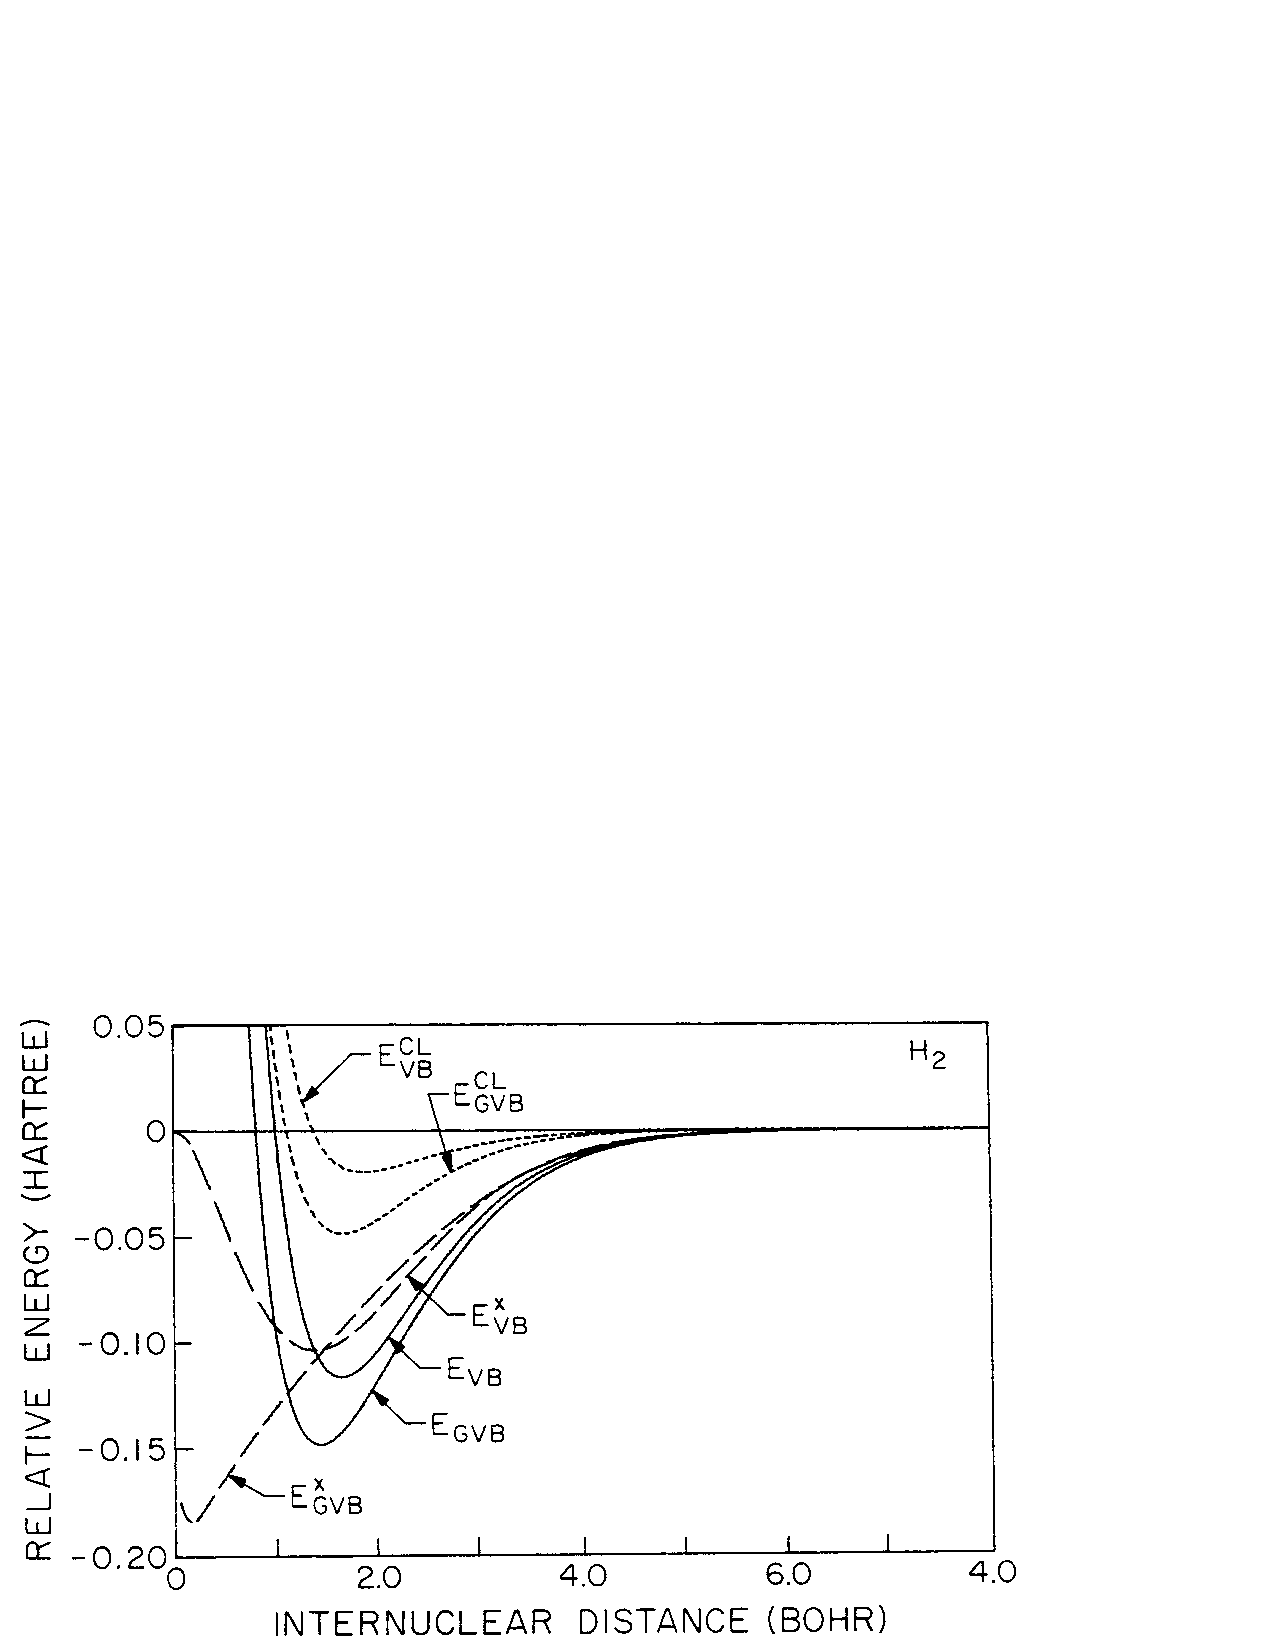
\includegraphics[scale=0.75]{fig3-24}
\caption{Comparison of the classical and exchange energies 
for the VB and GVB wave functions of H$_2$.}
\label{fig3-25}
\end{figure}

\noindent
In particular, for $R > R_e$, the $E^x$ is very nearly the same for
VB and GVB.  Thus, the main improvement
here is in the classical term, $E^{Cl}$. Similarly, in Figure
\ref{fig3-26} we see that it is the exchange part of the kinetic
energy that dominates the bonding energy.  Again, for $R > R_e$, we
see only minor changes in $T^x$ between VB and GVB.


\begin{figure}
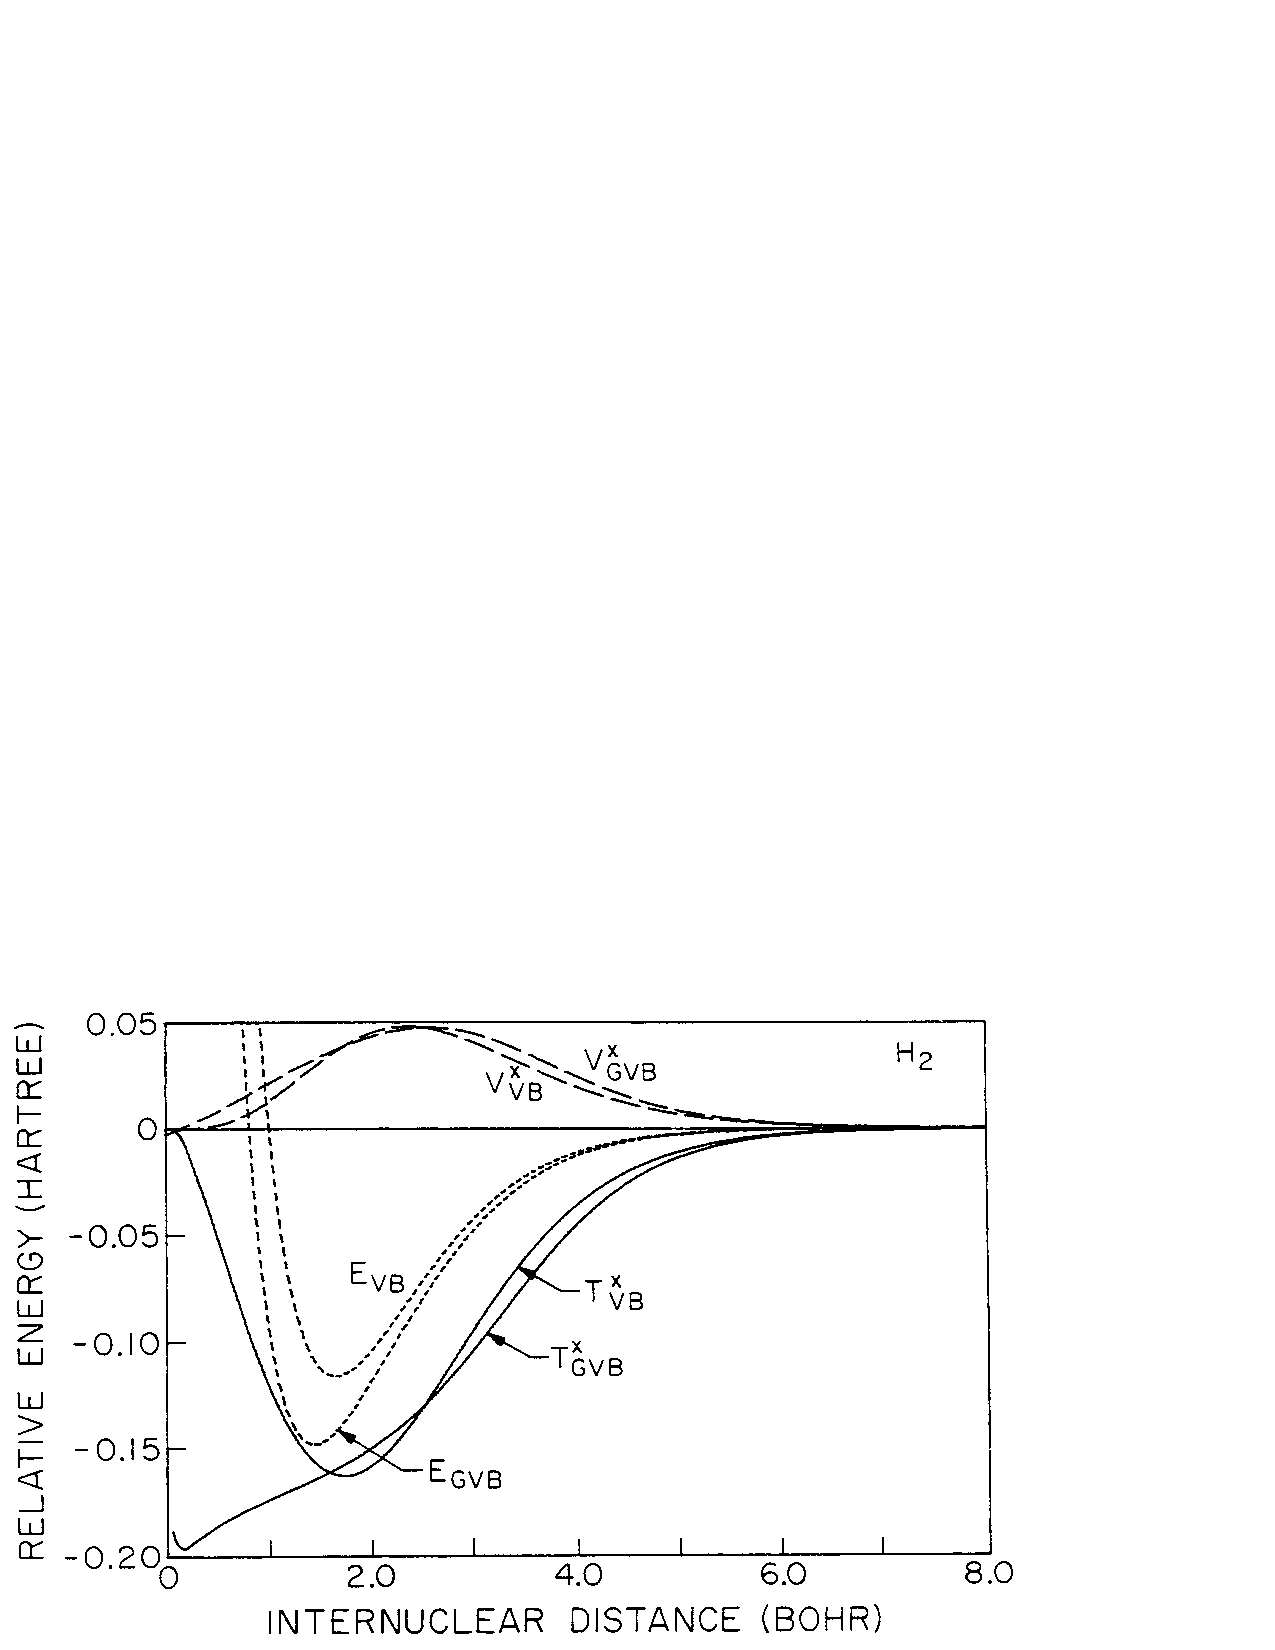
\includegraphics[scale=0.75]{fig3-25}
\caption{The kinetic and potential parts of $E^x$ for the 
VB and GVB wave functions of H$_2$}
\label{fig3-26}
\end{figure}

\subsection{CI Wavefunctions for H$_2$}

Earlier, we found that in He there are four important correlations each 
involving a correlating natural orbital having one nodal plane
\begin{eqnarray}
2s & ~ {\rm radial}\\
2p_x & ~ {\rm angular}\\
2p_y & ~ {\rm angular}\\
2p_x & ~ {\rm angular}\\
%%
\label{chap3-eqno67}
\end{eqnarray}
For H$_2$, the HF orbital is nodeless and again, we can find
four correlating natural orbitals each with one nodal plane.  These
are illustrated in Figure \ref{fig3-27}, where the names $1 \sigma_g$,
$1 \sigma_u$, etc., will be explained next.

\begin{figure}
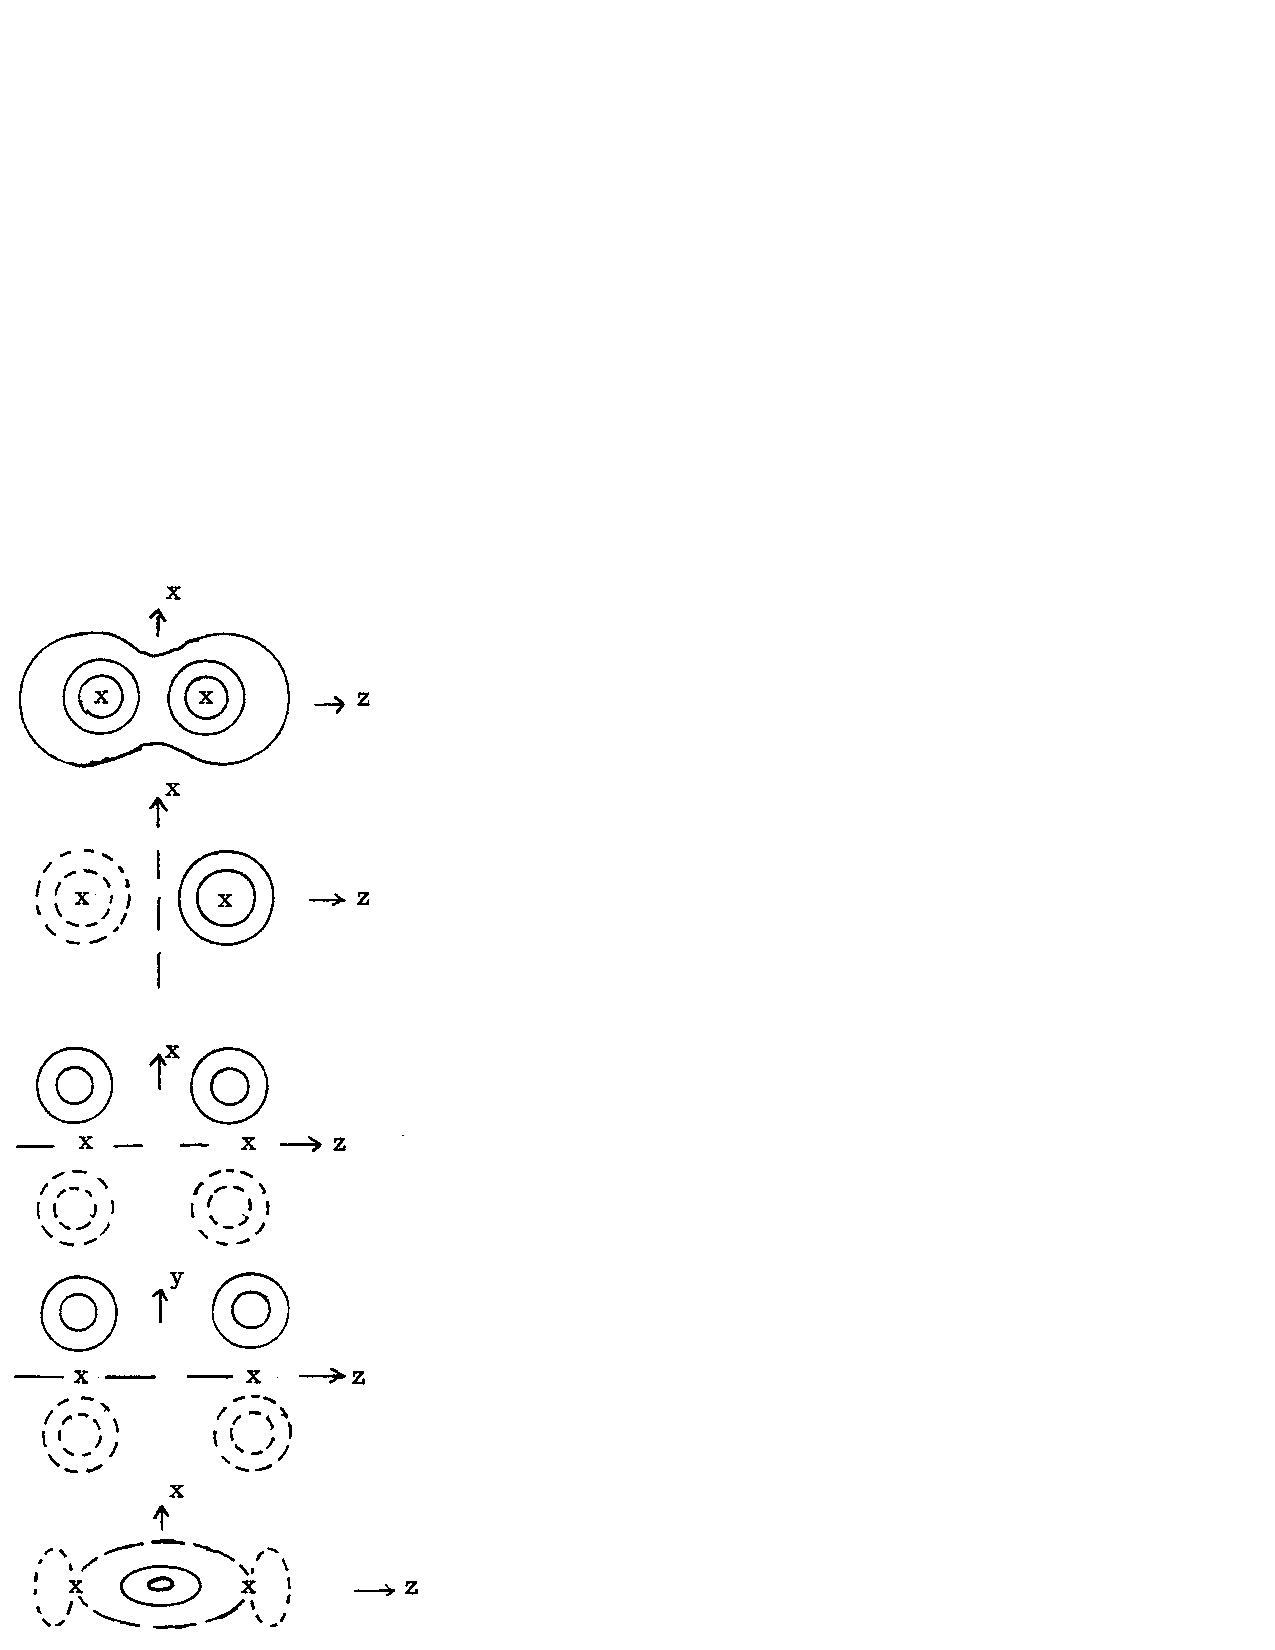
\includegraphics[scale=0.75]{fig3-26}
\caption{Correlating orbitals of H$_2$. Long dashes indicate nodal
planes, solid lines are positive  amplitudes and dotted lines negative
amplitudes.} 
\label{fig3-27}
\end{figure}

\noindent
As $R \rightarrow 0$, the H$_2$ orbitals change smoothly into (we say
that they \emph{correlate with}) the He orbitals in
(\ref{chap3-eqno67}), (H$_2$ on the left and He on the right)
\begin{eqnarray}
1 \sigma_g & \rightarrow 1s\\
2 \sigma_g & \rightarrow 2s\\
1 \sigma_u & \rightarrow 2p_z\\
1 \pi_{ux} & \rightarrow 2p_x\\
1 \pi_{uy} & \rightarrow 2p_y\\
\end{eqnarray}
and hence, the correlation effects are closely related, (H$_2$ on the
left and He on the right)
\begin{eqnarray}
{\rm left} - {\rm right} , ~ (1 \sigma_u) & \leftrightarrow {\rm 
angular}-z (p_z)\\
{\rm starboard} - {\rm portside} , ~ (1 \pi_{ux}) & \leftrightarrow {\rm 
angular}-x (p_x)\\
{\rm up} - {\rm down} , ~ (1 \pi_{uy}) & \leftrightarrow {\rm
  angular}-y (p_y)\\
{\rm in} - {\rm out} , ~ (2 \sigma_g) & \leftrightarrow {\rm radial}  
(2s)\\
\end{eqnarray}

The five dominant natural orbitals of H$_2$ are shown in Figure
\ref{fig3-28}, which should be compared to Figure \ref{fig3-16} for He.

\begin{figure}
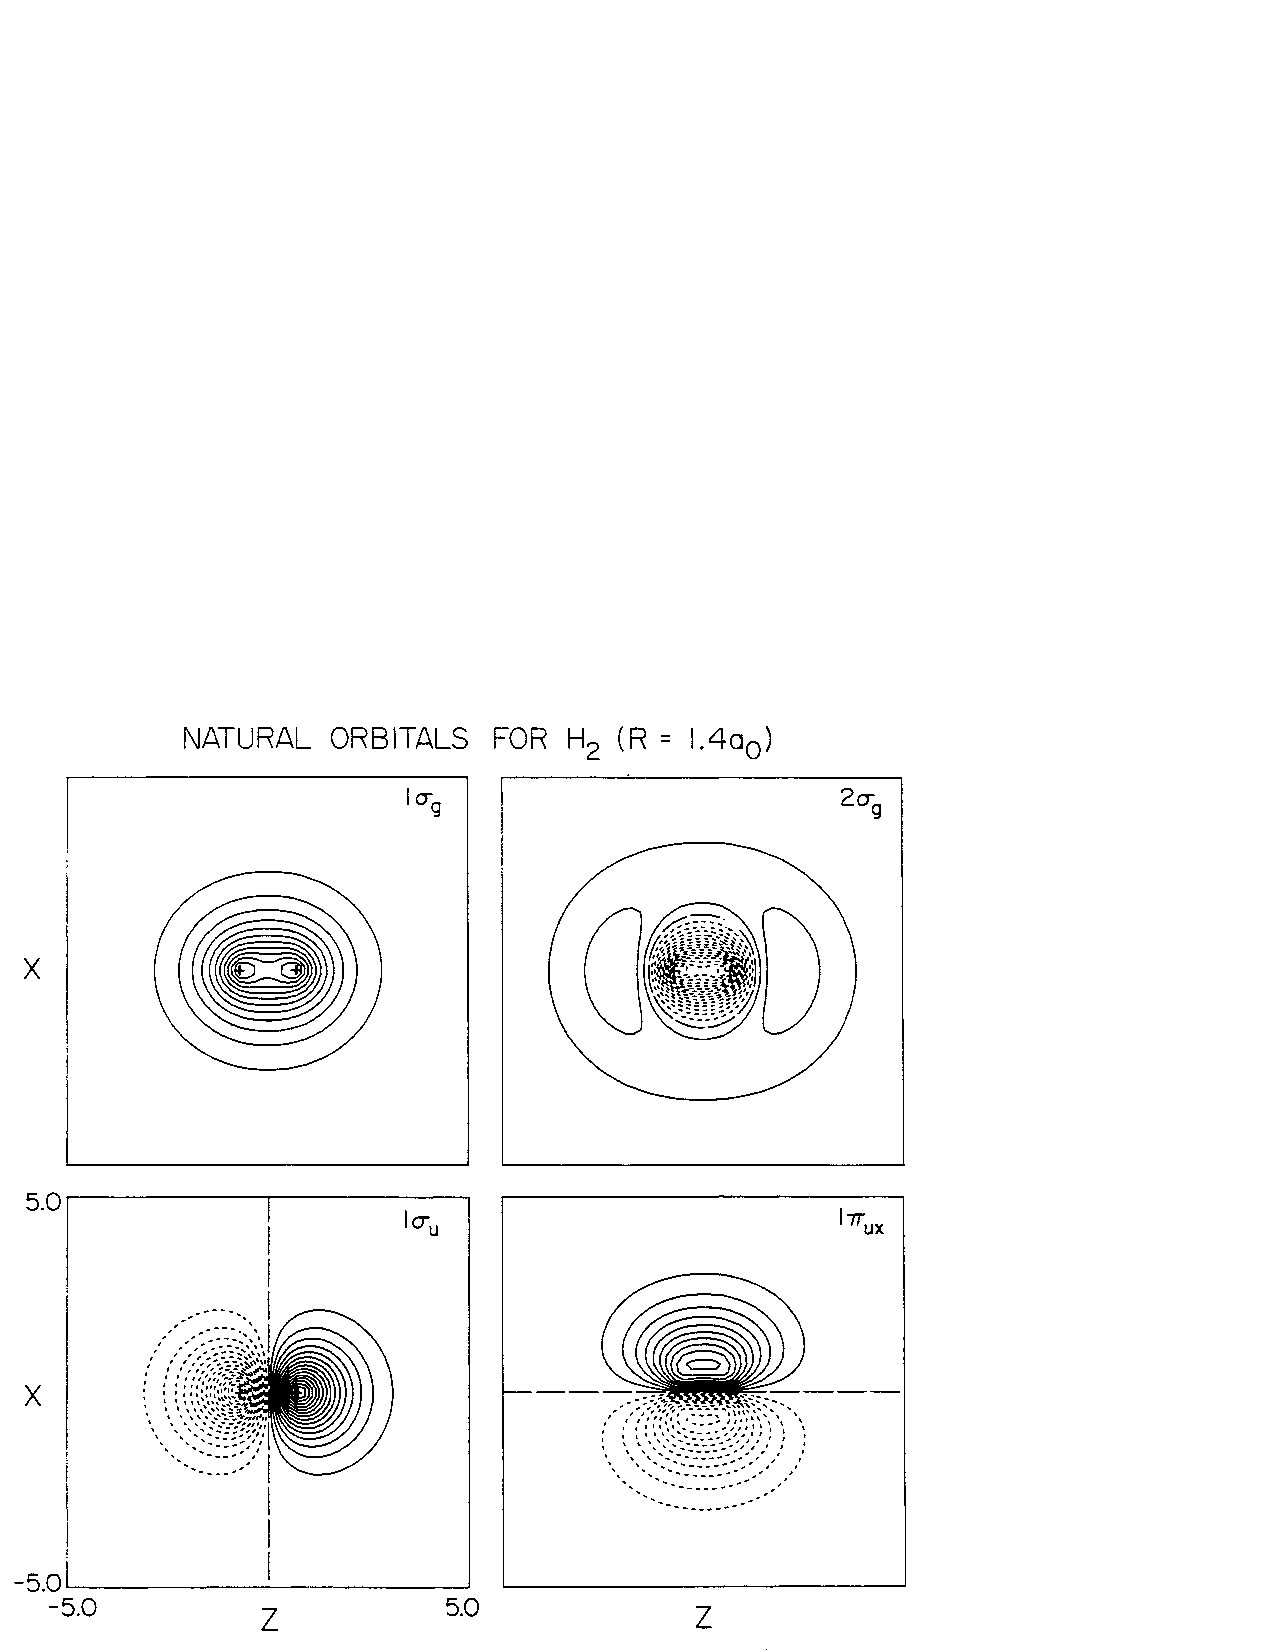
\includegraphics[scale=0.75]{fig3-27}
\caption{The natural orbitals of H$_2$ for $R = 1.4a_0$.$^{17}$.}
\label{fig3-28}
\end{figure}


With these five dominant natural orbitals, the wavefunction
\begin{eqnarray}
\Psi &=& C_{1 \sigma_g} \varphi_{1 \sigma_g} \varphi_{1 \sigma_g} - C_{2 
\sigma_g} \varphi_{2 \sigma_g} \varphi_{2 \sigma_g}\\ \nonumber
     && - C_{1 \sigma_u} 
\varphi_{1 \sigma_u} \varphi_{1 \sigma_u} - C_{1 \pi_u} \left[ \varphi_{1 
\pi_{ux}} \varphi_{1 \pi_{ux}} + \varphi_{1 \pi_{uy}} \varphi_{1 \pi_{uy}} 
\right]
\label{chap3-eqno68}
\end{eqnarray}
leads to an energy of $-$1.1699 h.  Comparing to the exact energy of
$-$1.1744 h, we see that wavefunction (\ref{chap3-eqno68}) accounts for
all but 4.5 mh = 0.12 eV 2.8 kcal of the exact energy. This is quite
adequate for our purposes and we will ignore all other terms. A more
complete analysis \cite{chap3-ref18} of CI calculations on H$_2$, for
$R = 1.4\ a_0$, in terms of natural orbitals is given in Table
\ref{table3-09}.


\begin{table}
\caption{Analysis of H$_2$ CI wavefunction 
in terms of natural orbitals.$^a$}
\label{table3-09}
\begin{tabular}{ccc}\\ \hline
Natural Orbital & Energy Lowering (mh) & \% $E_{corr}$\cr
$1 \sigma_u$ & 18.47 & 45.25\cr
$1 \pi_u$ & 10.34 & 26.56\cr
$2 \sigma_g$ & ?7.03 & 17.22\cr
$1 \pi_g$ & ?0.75 & 1.84\cr
$3 \sigma_g$ & ?0.51 & 1.25\cr
$2 \sigma_u$ & ?0.49 & 1.20\cr
$1 \delta_g$ & ?0.49 & 1.20\cr
$1 \pi_u$ & ?0.56 & 1.37\cr
$4 \sigma_g$ & ?0.29 & 0.71\cr
Totals & 39.43 & 96.60\cr \hline
\end{tabular} \\
$^a$See reference 18.  $^b$Total correlation energy is equal to 
0.04082 hartrees.
\end{table}

For the molecule at $R_e$, the dominant correlation is left-right. This becomes 
even more so for larger $R$.  Thus, at $R = \infty$, the exact wavefunction is
\begin{equation}
\Psi ( 1 , 2 ) = C_{1 \sigma_g} \varphi_{1 \sigma_g} \varphi_{1 \sigma_g} - 
C_{1 \sigma_u} \varphi_{1 \sigma_u} \varphi_{1 \sigma_u}
\end{equation}
where
\begin{equation}
C_{1 \sigma_g} = C_{1 \sigma_u} = {1 \over \sqrt{2}} ,
\end{equation}
\begin{equation}
\varphi_{1 \sigma_g} = {\left( \chi_{1sl} + \chi_{1sr} \right) \over 
\sqrt{2}} ,
\end{equation}
and
\begin{equation}
\varphi_{1 \sigma_u} = {\left( - \chi_{1sl} - \chi_{1sr} \right) \over 
\sqrt{2}} ,
\end{equation}
That is, only left-right correlation is present at $R = \infty$. For $R < 
0.8\ a_0$, in-out correlation becomes more important than left-right correlation.

\subsubsection{Notation}

For diatomic molecules, orbitals are classified in terms of their 
dependence upon $\varphi$, the angle of rotation about the molecular 
axis, $z$. Thus,
\begin{eqnarray}
\sigma & \Longrightarrow {\rm independent ~ of ~} \varphi\\
\pi_x & \Longrightarrow \cos \varphi\\
\pi_y & \Longrightarrow \sin \varphi\\
\end{eqnarray}
where $\varphi$ is referenced with respect to the $xz$ plane.

\section{Open Shell Wavefunction}

In Chapter 2, we found that the second and third states of H$_2$ have the form
\begin{equation}
{^1}\Phi = \varphi_g \varphi_u + \varphi_u \varphi_g
\end{equation}
and
\begin{equation}
{^3}\Phi = \varphi_g \varphi_u - \varphi_u \varphi_g
\end{equation}
where the orbitals $\varphi_g$ and $\varphi_u$ are orthogonal.  Such
wavefunctions, with orthogonal orbitals, are referred to as \emph{open
shell wavefunctions}. We will occasionally deal with such
wavefunctions and will analyze some aspects of the wavefunctions here.

The energies of the wavefunctions are
\begin{equation}
E = {N \over D}
\label{chap3-eqno69}
\end{equation}
where
\begin{equation}
{1 \over 2} D = \langle \varphi_g \varphi_u \vert \varphi_g \varphi_u
\pm \varphi_u \varphi_g \rangle = \langle \varphi_g \vert \varphi_g
\rangle \langle \varphi_u \vert \varphi_u \rangle \pm \langle
\varphi_g \vert \varphi_u \rangle \langle \varphi_u \vert \varphi_g
\rangle = 1
\end{equation}
\begin{equation}
{1 \over 2} N = \langle \varphi_g \varphi_u \vert H \vert \varphi_g 
\varphi_u \pm \varphi_u \varphi_g \rangle .
\label{chap3-eqno70}
\end{equation}
The first term of (\ref{chap3-eqno70}), is
\begin{eqnarray}
\langle \varphi_g \varphi_u \vert H \vert \varphi_g 
\varphi_u \rangle &= \langle g \vert h \vert g \rangle \langle u \vert u 
\rangle + \langle g \vert g \rangle \langle u \vert h \vert u 
\rangle + \langle gu \vert {1 \over R_{12}} \vert gu \rangle\\
& = \langle g \vert h g \rangle \langle u \vert h \vert u \rangle + 
J_{gu},\\
\end{eqnarray}
where $\langle \varphi_g \vert \varphi_u \rangle =0$ and the second
term is
\begin{eqnarray}
\pm \langle \varphi_g \varphi_u \vert H \vert \varphi_u \varphi_r 
\rangle = & \pm \left\{ \langle g \vert h \vert u \rangle \langle u 
\vert g \rangle + \langle g \vert u \rangle \langle u \vert h \vert g 
\rangle + \langle gu \vert {1 \over r_{12}} \vert ug \rangle 
\right\}\\
= & \pm K_{gu} .\\
\end{eqnarray}
Thus,
\begin{equation}
{^1}E - {^3}E = 2K_{gu} .
\end{equation}
Since $K_{gu} > 0$, the the ${^3}\Phi$ state is always below the ${^1}\Phi$ 
state.

The above analysis shows that the wavefunctions
\begin{equation}
\varphi_g \varphi_u \pm \varphi_u \varphi_g
\end{equation}
lead to an electron repulsion energy
\begin{equation}
E^{cl} \pm K_{gu} .
\end{equation}
Thus, the significance of the exchange integral $K_{gu}$ is that it is
the change in the energy upon superimposing the exchanged wavefunction
$\varphi^{(1)}_u \varphi^{(2)}_g$ or $\varphi^{(1)}_g
\varphi^{(2)}_u$. See Chapter 2.

\section{Appendices}

\subsection{Permutational Symmetry}
\label{chap3-app-a}

Since the Hamiltonian $H(1,2)$ for a two-electron system is invariant 
under permutation of electrons
\begin{equation}
H(2,1) = H(1,2)
\label{chap3app-eqno1}
\end{equation}
the exact eigenstates of $H$ are each either symmetric or antisymmetric 
under permutation.

For the proof, consider that $\Psi_0$ is an exact eigenfunction of
\begin{equation}
H(1,2) \Psi_0 (1,2) = E_0 \Psi_0 (1,2).
\label{chap3app-eqno2}
\end{equation}
Renumbering the electrons, this becomes
\begin{equation}
H(2,1) \Psi_0 (2,1) = E_0 \Psi_0 (2,1).
\label{chap3app-eqno3}
\end{equation}
But, using (\ref{chap3app-eqno1}) in (\ref{chap3app-eqno3}) leads to
\begin{equation}
H(1,2) \Psi_0 (2,1) = E+0 \Psi(2,1).
\label{chap3app-eqno4}
\end{equation}
Thus, for (\ref{chap3app-eqno2}) and (\ref{chap3app-eqno4}), both
$\Psi_0(1, 2)$ and $\Psi_0(2, 1)$ are eigenfunctions of $H(1,2)$, both
with the same energy.  There are two possibilities here. First there
are two, or more, different (linearly independent) state with energy
$E_0$, or there is only one state with energy $E_0$.

Where there is only one state with energy $E_0$, it must be that 
$\Psi_0(2, 1)$  is proportional to $\Psi_0(1, 2)$
\begin{equation}
\Psi_0(2, 1) = \lambda \Psi_0(1, 2).
\label{chap3app-eqno5}
\end{equation}
But interchanging 1 and 2 in (\ref{chap3app-eqno5}), leads to
\begin{equation}
\Psi_0(1, 2) = \lambda \Psi_0(2, 1)
\label{chap3app-eqno6}
\end{equation}
and substituting (\ref{chap3app-eqno6}) into (\ref{chap3app-eqno5}), leads
to
\begin{equation}
\Psi_0(2, 1) = \lambda^2 \Psi_0(2, 1).
\end{equation}
Thus, $\lambda = \pm 1$. That is, for a nondegenerate state, the 
wavefunction must be either symmetric, $\lambda = +1$,
\begin{equation}
\Psi^s (2,1) = \Psi^s (1,2) ,
\end{equation}
or antisymmetric, $\lambda = -1$,
\begin{equation}
\Psi^a (2,1) = \Psi^a (1,2),
\end{equation}
under permutation of the electrons, respectively.

Assuming now, that there are two or more different, linearly independent, 
states with energy $E_0$, we define new functions
\begin{equation}
\Psi^s_0 (1,2) = \Psi_0 (1,2) + \Psi (2,1)
\end{equation}
and
\begin{equation}
\Psi^a_0 (1,2) = \Psi_0 (1,2) - \Psi (2,1).
\end{equation}
Applying $H$, we obtain
\begin{equation}
H \Psi^s_0 = E_0 \Psi^s_0
\end{equation}
and
\begin{equation}
H \Psi^a_0 = E_0 \Psi^a_0
\end{equation}
and hence, the exact eigenfunctions of $H$ are, again, either 
symmetric or antisymmetric.

\subsection{Natural Orbitals}
\label{chap3-app-b}

A general CI wavefunction, for the ground state of a 
two-electron system
\begin{equation}
\Psi^s (1,2)  \ \sum^{P}_{\mu , \nu=1} C_{\mu \nu} \chi_{\mu} (1) 
\chi_{\nu} (2)
\label{chap3app-eqno7}
\end{equation}
can always be rewritten in terms of doubly-occupied orbitals
\begin{equation}
\Psi^s (1,2)  \ \sum^{P}_{\mu =1} {\bar C}^Z_{\mu \mu} {\bar \chi}_{\mu} (1) 
{\bar \chi}_{\mu} (2)
\label{chap3app-eqno8}
\end{equation}
where the natural orbitals $\{ {\bar \chi}_{\mu}\}$ are linear combinations 
of the original basis functions $\{ \chi_{\mu} \}$.

The proof is that since $\psi^s$ is symmetric, the coefficient matrix is 
symmetric
\begin{equation}
C_{\mu \nu} = C_{\nu \mu}
\end{equation}
If we choose new basis functions
\begin{equation}
\left\{ {\bar \chi}_{\mu} ; \mu = 1 , \cdot \cdot \cdot P \right\}
\end{equation}
that are linear combinations of the old function
\begin{equation}
\left\{ \chi_{\mu} ; \mu = 1 , \cdot \cdot \cdot P \right\}
\end{equation}
\begin{equation}
\chi_{\mu} = \sum_{\nu} V_{\mu \nu} {\bar \chi}_{\nu},
\end{equation}
then the wavefunction (\ref{chap3app-eqno7}) becomes
\begin{equation}
\Psi^s = \sum_{\mu \nu ,\sigma \eta} C_{\mu \nu} V_{\mu \sigma} 
{\bar \chi}_{\sigma} (1) V_{\nu \eta} {\bar \chi}_{\eta} (2) = 
\sum_{\sigma \eta} {\bar C}_{\sigma \eta} {\bar \chi}_{\sigma} (1) 
{\bar \chi}_{\eta} (2)
\end{equation}
where
\begin{equation}
{\bar C}_{\sigma \eta} = \sum_{\mu , \nu} V_{\mu \sigma} C_{\mu 
\nu} V_{\nu \eta} .
\end{equation}
The wavefunction $\Psi^s$ is unchanged by this transformation of the basis, 
but in the new basis, the CI expansion coefficients 
are different.

In matrix notation, the new coefficients are given by
\begin{equation}
\mathbf{\bar C} = \mathbf{{\tilde V}CV}
\end{equation}
Since $\mathbf{C}$ is a real symmetric matrix, there is always some 
transformation $\mathbf{V}$ for which the transformed matrix 
$\mathbf{\bar C}$ is diagonal.  Thus, there is always a particular choice 
of basis functions such that
\begin{equation}
\Psi^s = \sum^{P}_{\mu =1} {\bar C}_{\mu \mu} {\bar \chi}_{\mu} (1) 
{\bar \chi}_{\mu} (2)
\label{chap3app-eqno9}
\end{equation}
With this basis, there are only $P$ terms in the CI expansion rather
than $P^2$ as in (\ref{chap3app-eqno7}).  Thus, (\ref{chap3app-eqno9})
is a much simpler wavefunction.  To find the $V$ leading to the
natural orbitals, we must first solve the CI equations to find
$\mathbf{C}$.  Hence, the natural orbitals do not help us solve for
the CI wavefunction.  However, having obtained a CI wavefunction, we
will immediately transform to the natural orbitals in order to discuss
and interpret the wavefunction.

\subsection{Evaluating Energy Quantities for Atoms}
\label{chap3-app-c}

Here we consider the evaluation of the various energy quantities for a 
two-electron system, with both electrons in the same $1s$ orbital,
\begin{equation}
\varphi_{1s} = Ne^{- \zeta r}
\end{equation}
where the orbital exponent $\zeta$ is variable.

\subsubsection{One Electron Quantities}

First the normalization coefficient, $N$, is obtained from
\begin{equation}
1 = \langle \varphi_{1s} \vert \varphi_{1s} \rangle = N^2 
\int dx\ dy\ dz\ e^{-2 
\zeta r} = 4 \pi N^1 \int\limits^{\infty}_{0} r^2 dr\ e^{-2 \zeta r} = 
{4 \pi \over (2 \zeta )^3} N^2 \int\limits^{\infty}_{0} \rho^2 d \rho 
\ e^{- \rho} = {8 \pi \over 8 \zeta^3} N^2 ,
\end{equation}
so that
\begin{equation}
N = \sqrt{{\zeta^3 \over \pi}} .
\end{equation}
The nuclear attraction terms are
\begin{eqnarray}
V^{en}_{1s} = \langle 1s \vert - {Z \over r} \vert 1s 
\rangle &= - ZN^2 \int\limits^{\infty}_{0} rdr\ e^{-2 \zeta r} 
\int\limits^{\pi}_{0} \int\limits^{2 \pi}_{0} \sin \theta d \theta d 
\varphi\cr
&= - {ZN^2 4 \pi \over 4 \zeta^2} = - \zeta Z\cr
%
\label{chap3app-eqno10}
\end{eqnarray}

The kinetic energy term is obtained, most simply, by noting that
\begin{equation}
\nabla \varphi_{1s} = - \zeta \varphi_{1s} {\hat e}_r
\end{equation}
where ${\hat e}_r$ is a unit vector in the $r$ direction, and hence
\begin{equation}
T_{1s} = \langle 1s \vert t \vert 1s \rangle = \langle 
1s \vert - {1 \over 2} \nabla^2 \vert 1s \rangle = {1 \over 2} 
\langle \nabla \varphi_{1s} \cdot \nabla \varphi_{1s} \rangle = {1 \over 
2} \zeta^2 \langle \varphi_{1s} \vert \varphi_{1s} \rangle = {1 \over 2} 
\zeta^2
\label{chap3app-eqno11}
\end{equation}

To check these quantities consider He$^+$ where $\zeta = 2$. In this
case, (\ref{chap3app-eqno10}) and (\ref{chap3app-eqno11}) lead to
\begin{equation}
E_{1s} = T_{1s} + V^{en}_{1s} = {1 \over 2} \zeta^2 - \zeta Z
\end{equation}
where $Z = 2$.  Optimizing $\zeta$, leads to $\zeta = Z$, and hence,
\begin{equation}
E_{1s} = - {1 \over 2} Z^2
\end{equation}
both of which are correct.

\subsubsection{Two Electron Quantities}

For He, we also need the two-electron interaction term
\begin{equation}
J_{1s , 1s} = \langle \varphi_{1s} \varphi_{1s} \vert {1 \over r_{12}} 
\vert \varphi_{1s} \varphi_{1s} \rangle = \langle \varphi_{1s} \vert J_{1s} 
\varphi_{1s} \rangle ,
\label{chap3app-eqno12}
\end{equation}
where
\begin{equation}
J_{1s} (1) = \int dx_2\ dy_2\ dz_2 {1 \over r_{12}} \vert \varphi_{1s} (2) 
\vert^2
\label{chap3app-eqno13}
\end{equation}
is the Coulomb field evaluated at $r_1$ due to an electron, called 2, in the 
$1s$ orbital.

The complication in evaluating such integrals as $J_{1s , 1s}$ is that
the integrand of (\ref{chap3app-eqno13}) depends on $R_{12}$.  The usual
solution is to use the Laplace expansion
\begin{equation}
{1 \over r_{12}} = \sum^{\infty}_{l=0} {r^l_< \over r^{l+1}_>} P_\ell 
\left( \cos \theta_{12} \right)
\label{chap3app-eqno14}
\end{equation}
where $r_< = r_1$ if $r_1 < r_2$ or $r_< = r_2$ if $r_2 < r_1$, and
oppositely for $r_>$.  With (\ref{chap3app-eqno14}),
(\ref{chap3app-eqno13}) becomes
\begin{equation}
J_{1s} = \sum^{\infty}_{l=0} \left\{ \int\limits^{\infty}_{0} {r^l_< 
\over r^{l+1}_>} r^2_2 dr_2 \vert \varphi_{1s} (2) \vert^2 
\int\limits^{\pi}_{0} \sin \theta d \theta P_\ell \left( \cos \theta 
\right) \int\limits^{2 \pi}_{0} d \varphi \right\}.
\label{chap3app-eqno15}
\end{equation}
The integration over $\theta$ is zero unless $l = 0$, so that
(\ref{chap3app-eqno15}) becomes
\begin{equation}
J_{1s} (1) = 4\pi \int\limits^{\infty}_{0} {r^2_2 dr_2 \over r_>} 
\vert \varphi_{1s} (2) \vert^2 = 4 \pi \left\{ {1 \over r_1} 
\int\limits^{r_1}_{0} r^2_2 dr_2 \vert \varphi_{1s} (2) \vert^2 + 
\int\limits^{\infty}_{0} r_2 dr_2 \vert \varphi_{1s} (2) \vert^2 
\right\}
\label{chap3app-eqno16}
\end{equation}
Before proceeding to evaluate $J_{1s}(1)$, one should notice that
(\ref{chap3app-eqno16}) is a well-known result in electrostatic. The
quantity
\begin{equation}
Q_1 = 4 \pi \int\limits^{r_1}_{0} r^2_2 dr_2 \vert \varphi_{1s} (2) \vert^2
\end{equation}
is just the part of the charge distribution inside the point $r_1$.
According to (\ref{chap3app-eqno16}), the total contribution of this
spherically symmetric charge distribution inside $r_1$, is the same
value
\begin{equation}
{1 \over r_1} Q_1
\end{equation}
as if all the charge, $Q_1$, were localized at the nucleus.  Letting
\begin{equation}
Q_2 (r) = 4 \pi r^2 \vert \varphi_{1s} (r) \vert^2 ,
\end{equation}
the quantity $Q_2(r)dr$ is the charge on the spherical shell of radius
$r$, and thickness $dr$.  According to (\ref{chap3app-eqno16}), the
contribution of this charge to the potential is
\begin{equation}
{1 \over r} Q_2 (r) dr
\end{equation}
and is the same for all $r_1$ inside $r$.

Grunging on, we find
\begin{equation}
Q_1 = 4 \pi N^2 \int\limits^{r_1}_{0} r^2_2 dr_2 e^{-2 \zeta r_2} = 
{4 \pi N^2 \over (2 \zeta )^3} \int\limits^{\rho_1}_{0} \rho^2 d \rho 
e^{- \rho}
\end{equation}
where $\rho_1 = 2 \zeta r_1$.  Integrating by parts, this becomes
\begin{equation}
Q_1 = \left[ 1 - e^{- \rho_1} \left( 1 + \rho_1 + {1 \over 2} 
\rho^2_1 \right) \right] .
\end{equation}
Similarly, the second term of (\ref{chap3app-eqno16}) is
\begin{equation}
I_2 = 4 \pi N^2 \int\limits^{\infty}_{r_1} r_2 d r_2 e^{- 2 \zeta 
r_2} = \zeta \left[ \rho_1 e^{- \rho_1} + e^{- \rho_1} \right] .
\end{equation}
Thus
\begin{equation}
J_{1s} (1) = {1 \over r_1} Q_1 + I_2 = {1 \over r_1} \left( 1 - e^{-2 
\zeta r_1} \right) - \zeta e^{-2 \zeta r_1}.
\label{chap3app-eqno17}
\end{equation}
For large $r_1$, this becomes
\begin{equation}
J_{1s} = {1 \over r_1}
\end{equation}
as expected, and for small $r_1$ we obtain
\begin{equation}
J_{1s} (1) = \zeta - {2 \over 3} \zeta^3 r^2_1 + O (r^3_1 )
\end{equation}
Thus, $J_{1s}$ has the form in Figure \ref{fig3-29}.

\begin{figure}
\begin{center}
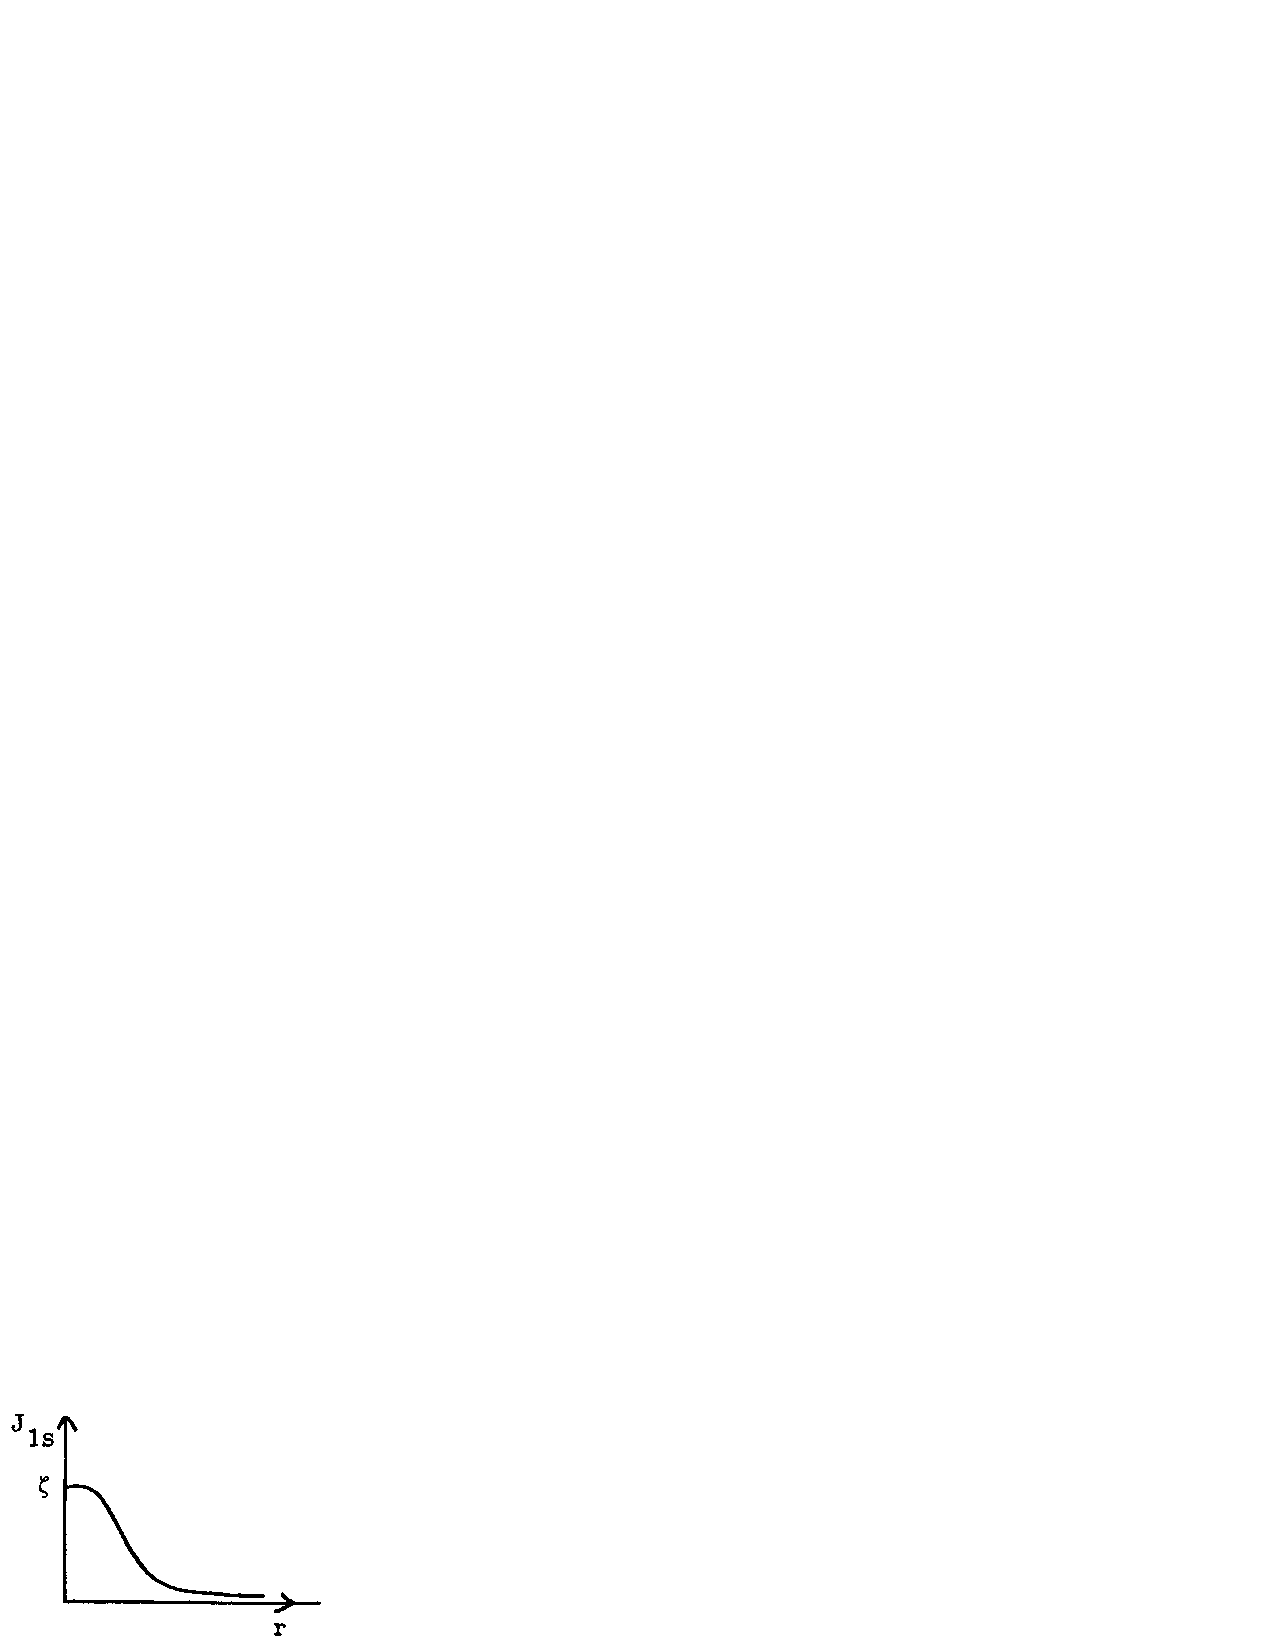
\includegraphics[scale=0.75]{fig3-28}
\end{center}
\caption{The Coulomb potential $J_{1s} (r)$.}
\label{fig3-29}
\end{figure}


Using (\ref{chap3app-eqno17}) in (\ref{chap3app-eqno12}), we obtain
\begin{eqnarray}
J_{1s , 1s} &= 4 \pi N^2 \int\limits^{\infty}_{0} r^2 dre^{-2 \zeta r} 
\left[ {1 \over r} - {1 \over r} e^{-2 \zeta r} - \zeta e^{-2 \zeta 
r} \right]\cr
&= 4 \zeta^3 \left\{ {1 \over (2 \zeta )^2} - {1 \over (4 
\zeta )^2} - {2 \zeta \over (4 \zeta )^3} \right\} = {5 \over 8} 
\zeta\cr
\end{eqnarray}

\medskip

\subsubsection{Qualitative Analysis of $J_{1s , 1s}$}

Defining the average size, ${\bar r}$, for the $\varphi_{1s}$ orbital as
\begin{equation}
\langle \varphi_{1s} \vert {1 \over r} \vert \varphi_{1s} \rangle = {1 \over 
{\bar r}}
\end{equation}
we see from (\ref{chap3app-eqno16}) that
\begin{equation}
{\bar r} = {1 \over \zeta} .
\end{equation}
An approximate value of $J_{1s ,1s}$ can be obtained by assuming each 
electron is at its average radius, ${\bar r} = 1 / \zeta$, and averaging 
over the distances between these electrons, assuming each to be on the 
sphere of radius ${\bar r}$.  If the instantaneous location of electron 1 
is taken to define the $z$ axis, then the average position of electron 2 
will be approximately in the $xy$ plane.  This leads to
\begin{equation}
{\bar r}_{12} \approx \sqrt{2} {\bar r}
\end{equation}
and, hence, to
\begin{equation}
J_{1s , 1s} = {1 \over \sqrt{2} {\bar r}} = {1 \over \sqrt{2}} 
\zeta = 0.707 \zeta
\end{equation}
The exact value is $J_{1s , 1s} = 0.625 \zeta$ so that the above estimate is 
only about 10 percent high.

\subsection{The Exact Wavefunction of H$^+_2$}
\label{chap3-app-d}

In order to solve for the exact wavefunction of H$^+_2$, we use 
elliptic coordinates
\begin{equation}
\xi = {(r_a + r_b ) \over R} ,
\end{equation}
\begin{equation}
\eta = {(r_a - r_b ) \over R} ,
\end{equation}
and $\varphi$ equal to azimuthal angle as defined in 
Chapter 2.  With elliptic coordinates, the Hamiltonian for H$^+_2$ 
becomes separable, expressible as a sum of terms each depending on 
a different variable. Hence, the exact wavefunction of H$^+_2$ can be 
factored into terms, each depending upon different variables,
\begin{equation}
\Psi ( \xi , \eta , \varphi ) = \Lambda ( \xi ) M ( \eta ) \Phi ( 
\varphi) .
\end{equation}
For the ground state of H$^+$ at $R = 2a_0$, the resulting, unnormalized 
wavefunction is$^2$
\begin{equation}
\Lambda ( \xi ) = ( 1 + \xi )^{0.34679} ( 1 + 0.0168 \delta + 0.0004 
\delta^2 )e^{- 1.48501 \xi} ,
\end{equation}
\begin{equation}
M( \eta) = \left[ 1.1450P_0 (\eta) + 0.29844P_2(\eta) + 
0.011461P_4(\eta) + 0.000184P_2(\eta) + 0.000002P_8(\eta) \right] ,
\end{equation}
\begin{equation}
\Phi ( \varphi) = 1,
\end{equation}
where
\begin{equation}
\delta = { ( \xi - 1 ) \over ( 1 + \xi)}
\end{equation}
and $P_\ell ( \eta )$ are Legendre polynomials $[P_0 = 1 , P_2 = {1
\over 2} ( 3 \eta^2 ),\cdots]$.  For comparison, the MBS wavefunction
in elliptic coordinates is
\begin{equation}
\psi^{MBS} = \left( e^{- \zeta r_a} + e^{- \zeta r_b} \right) = 
\left[ e^{\zeta {R \over 2} \eta} + e^{- \zeta {R \over 2} \eta} 
\right] e^{- \zeta {R \over 2} \xi}
\end{equation}
corresponding to
\begin{equation}
\Lambda ( \zeta ) = e^{-1.23 \zeta}
\end{equation}
and
\begin{equation}
M( \eta ) = \cos h ( 1.23 \eta )
\end{equation}
at $R = 2\ a_0$ (the optimum $\zeta$ at $R = 2\ a_0$ is $\zeta =
1.23$).  At $R = 2$, the MBS wavefunction leads to $\zeta = 1.23$,
somewhat more diffused than the 1.485 for the exact wavefunction. The
optimum energy and bond lengths for the exact wavefunction are listed
in Table \ref{table3-01}.

When we say \emph{exact} here, we are referring to the exact solutions
of (\ref{chap3app-eqno10}) and (\ref{chap3app-eqno11}).  However,
(\ref{chap3app-eqno10}) and (\ref{chap3app-eqno11}) do not lead to an
exact description of H$^+_2$.  The two main assumptions here are,
first, the neglect of the nuclear kinetic energy terms, referred to as
Born-Oppenheimer breakdown, and, secondly, neglect or relativistic
effects.  Inclusion of nuclear kinetic energy leads to corrections of
order $1/2M$, where $M$ is the proton mass, in Hartree atomic units,
e.g., $1/2M =$ 0.0003 h = 0.007 eV.  The actual correction to the energy
at $R_e$ from the nuclear kinetic energy terms, see Table
\ref{table3-01}, is $+ .00085$ h = 0.023 eV = 0.53 kcal, and from the
relativistic effects is .000005 h = 0.00013 eV = 0.003 kcal.  In order
to compare with experiment, such terms must be included, actually, for
H$^+_2$ the experimental results are not yet precise enough to require
these corrections.  However, in this course we will generally ignore
such effects and will refer only to results of nonrelativistic, fixed
nuclei calculations.

